% Paper template for Advanced Physics Laboratory Course
% Made by Alice Pagano and Francesca Dodici

\documentclass[rmp,10pt,onecolumn,fleqn,notitlepage]{revtex4-1}

% LOAD PACKAGES

% GENERAL PACKAGES
\usepackage{graphicx}
\usepackage{wrapfig}
\usepackage{color}
\usepackage{latexsym,amsmath}
\usepackage{physics}
\usepackage{chemformula}
\usepackage{tabularx}
\usepackage{float}
\usepackage{siunitx}
\usepackage{amssymb}
\usepackage[caption=false, justification=right]{subfig} % rovina la formattazione delle figure se caption=true
\usepackage{multirow}
\usepackage{subcaption}
\usepackage{comment}
% LISTING PACKAGES
\usepackage{xcolor}
\usepackage{listings}
\usepackage{framed}
\usepackage{inconsolata} % To change the listing font

% URL PACKAGE AND SETTING
\definecolor{linkcolor}{rgb}{0,0,0.65} %hyperlink
\definecolor{linescolor}{rgb}{0.65,0.16,0.16}
\definecolor{cool}{RGB}{49,54,149}
\definecolor{hot}{RGB}{165,0,38}
\usepackage[pdftex,colorlinks=true, pdfstartview=FitV, linkcolor= linescolor, citecolor= linescolor, urlcolor= linkcolor, hyperindex=true,hyperfigures=true]{hyperref} %hyperlink%

% PAGE SETTING
\usepackage{fancyhdr} 

\pagestyle{fancyplain}
\fancyhf{}
\fancyfoot[R]{\textbf{\thepage}}
\fancyfoot[L]{Università degli Studi di Padova - Dipartimento di Fisica e Astronomia Galileo Galilei} 
%\fancyhead[L]{\textbf{Advanced Physics Laboratory Report}}
\fancyhead[L]{\ifnum\value{section}>0\nouppercase{\textbf{\leftmark}\fi}}
\fancyhead[R]{\textbf{Rosa Maria Guizzetti - Enrico Lupi}}
\renewcommand{\headrulewidth}{0.2pt}
\renewcommand{\footrulewidth}{0.1pt}

\setlength\parindent{9pt} % To adjust the intendation

% SECTION STYLE
%Redefine \thesubsection as \thesection.\alph{subsection}. (\alph replaces the default \arabic; you could also choose, e.g., \Alph, \roman, and \Roman.)
\renewcommand{\thesection}{\textbf{\Roman{section}}}
\renewcommand{\thesubsection}{\textbf{\arabic{subsection}}}
\renewcommand{\thesubsubsection}{\textbf{\Alph{subsubsection}}}
%\renewcommand{\thesection}{\textbf{\arabic{section}}}
%\renewcommand{\thesubsection}{\thesection.\textbf{\arabic{subsection}}}
%\renewcommand{\thesubsubsection}{\textbf{\thesection.\arabic{subsection}.\arabic{subsubsection}}}

% FIGURE AND TABLE STYLE
\renewcommand{\tablename}{\textbf{TAB.}}
\renewcommand{\thetable}{\textbf{\arabic{table}}}
\renewcommand{\figurename}{\textbf{FIG.}}
\renewcommand{\thefigure}{\textbf{\arabic{figure}}}

% BIBLIOGRAPHY FILE AND SETTING
\bibliographystyle{aipnum4-1}
\setcitestyle{numbers,square}






\begin{document}

% SET FIGURE CAPTION IN BOLD
\captionsetup[figure]{labelfont={bf},labelformat={default},labelsep=period,name={FIG.}}


% FRONTESPIZIO

% Insert logo images above
\begin{figure}[H]
\begin{minipage}{0.25\linewidth}

\includegraphics[width=\linewidth]{Images/logo/logo_DFA.jpg}
\end{minipage}
\hfill
\begin{minipage}{0.35\linewidth}

\includegraphics[width=\textwidth]{Images/logo/unipdwhite.png}
\end{minipage}
\end{figure}

% Make upper lines
\noindent\makebox[\linewidth]{\color{linescolor} \rule{0.85\paperwidth}{1.2 pt}}
\noindent\makebox[\linewidth]{\color{linescolor} \rule[0.3cm]{0.85\paperwidth}{1pt}}

% Title
\title{$\boldsymbol{LaBr_3(Ce)}$ Scintillation Detector Characterization}
\author{Rosa Maria Guizzetti - 2089389 - rosamaria.guizzetti@studenti.unipd.it \\ Enrico Lupi - 2090596 - enrico.lupi@studenti.unipd.it}
\date{\today}

% Abstract
\begin{abstract}

Scintillation detectors are commonly used for measuring the cross section of reactions relevant in astrophysics, since they provide high efficiencies at the expense of sub-optimal energy resolution and internal background. This work will focus on the complete characterization of a system of two LaBr detectors in terms of energy resolution and efficiency. Time resolution and coincidences will also be investigated.


\end{abstract}

% Make title
\maketitle

% Make lower line
\noindent\makebox[\linewidth]{\color{linescolor} \rule[0.1cm]{0.85\paperwidth}{1pt}}


% INDEX

% Index configuration
{
  \hypersetup{linkcolor=black}
  \tableofcontents
}
% Make lower lines
\noindent\makebox[\linewidth]{\color{linescolor} \rule[-0.2cm]{0.85\paperwidth}{1pt}}
\noindent\makebox[\linewidth]{\color{linescolor} \rule[0.3cm]{0.85\paperwidth}{1.2 pt}}
\pagebreak


% Page configuration: start counting page after the first one which is the title
\pagenumbering{gobble} 
\newpage
\pagenumbering{arabic}




\section{Introduction}
\label{sec:introduction}

Scintillators are frequently used for measuring the cross section of reactions relevant in astrophysics. This type of detectors provide high efficiencies at the cost of not optimal energy resolution and internal background, compared to usual $\gamma$-spectroscopy detectors as HPGe.  \\

The working principle of scintillators is the following. When stricken by gamma-ray, the primary electrons raise secondary electrons to the conduction band, leaving holes in the valence band. 
If the electrons are allowed to de-excite by falling back to the valence band, they will emit electromagnetic radiation, and if this radiation is in, or near, optical wavelengths, it can be detected by a photomultiplier or other lightmeasuring
device to provide the detector signal.

It may happen that the band gap is large and photons emitted by de-excitation of electrons directly from the conduction band would be far outside of the
visible range, making the detection of the light difficult. Furthermore, the bulk of the material absorbs the emitted photons before they reach the photomultiplier. Both problems are solved by using an activator. The ground state of these activator sites lies just above the valence band and the excited states somewhat below the conduction band. This means that the photon energy released when these levels de-excite will be lower and the electromagnetic radiation will be of a longer wavelength, perhaps in the visible range. It also means that the emission wavelength will no longer match the absorption characteristics of the scintillator and so much less light will be lost before measurement by the
photomultiplier. \\


The ideal scintillator material for gamma-ray
detection and spectrometry must have the following properties:
\begin{itemize}
    
    \item there must be a reasonable number of electron–hole pairs produced per unit of gamma-ray energy;
    
    \item it would be very desirable for the material to have a high stopping power for gamma radiation (which means, in practice, high density and atomic number);

    \item for spectrometry, the response must be proportional to energy;

    \item the scintillator must be transparent to the emitted light;

    \item the decay time of the excited state must be short to allow high count rates;

    \item the material should be available in optical quality in reasonable amounts at reasonable cost;

    \item the refractive index of the material should be near to that of glass (ca. 1.5) to permit efficient coupling to photomultipliers.
    
\end{itemize}


In this work, two $LaBr_3(Ce)$ (Cerium activated Bromide of Lanthanum) detectors will be studied. This material provides several advantages over the more common $NaI(Tl)$, namely a greater light output, better resolution, shorter scintillation decay time and higher efficiency due to its higher density.
A single disadvantage is its inherent radioactive impurity content due to Lanthanum's naturally
occurring radioisotope, $^{138}La$. \cite{gilmore_2008}\\

The two detectors will be first calibrated using three different radioactive sources.
Afterward, we will study their energy resolution and timing performances in coincidence. Lastly, their efficiency will be computed using different methods.

\section{Experimental Set-up}
\label{sec:setup}

The investigated $LaBr_3(Ce)$ detectors are cylindrical crystals of 9.8 cm diameter aligned at 180° in front of each other (fig. \ref{fig:setup}). The detectors are coupled with photomultipliers powered at 690-650 V. The output of the PMTs is directly read by a CAEN DT5730 digitizer equipped with DPP-PSD firmware, read in turn by the CoMPASS software. Henceforth, we will distinguish the two detectors by referring to them as \emph{channel 0} and \emph{channel 1}. \\

The radioactive sources used are: Cobalt-60, Cesium-137 and Sodium-22. The samples' actvities are 376 kBq, 389 kBq and 418 kBq respectively, with an error of 3\%. The samples are located in the middle of the two detectors. 
For each sample, a run is recorded at each of the following distances: 10 cm, 15 cm and 20 cm. An additional run, for a total of 10, is taken without any source to record the internal background.
	
\begin{figure}[h!]
\centering
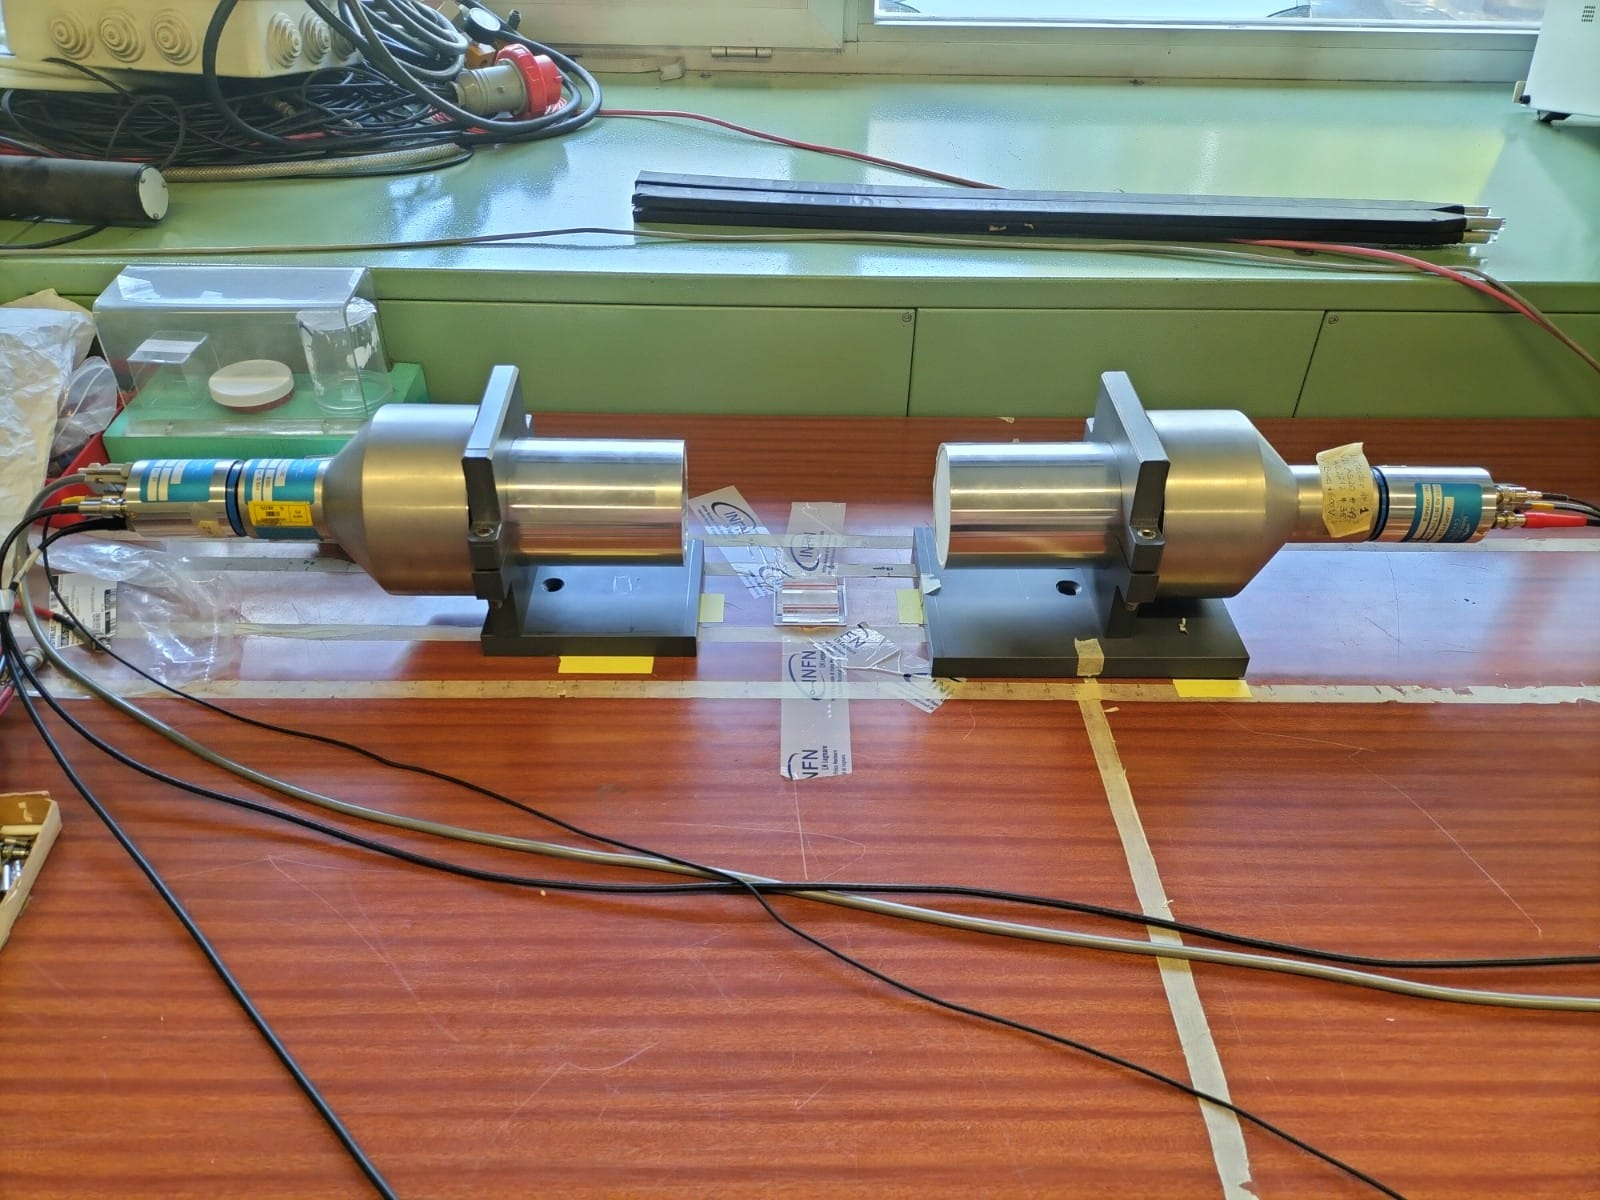
\includegraphics[width=0.6\textwidth]{Images/lab/Calibration.jpeg}
\caption{Photo of the detector set-up.}
\label{fig:setup}
\end{figure}

\section{Energy Calibration}
\label{sec:calibration}

The first step is to calibrate the energy response of the detectors. In order to do so, we will use the photopeaks of the radioactive sources: 1173.84 and 1331.70 keV for $^{60}$Co and 661.65 keV for $^{137}$Cs. The position of the peaks is obtained by fitting the energy spectra with a gaussian fit over a linear background (figs. \ref{fig:calib_Co} and \ref{fig:calib_Cs}), and then averaged across the different distances. 


\begin{figure}[H]
	\begin{minipage}[c]{0.5\linewidth}
	\subfloat[][Channel 0.]{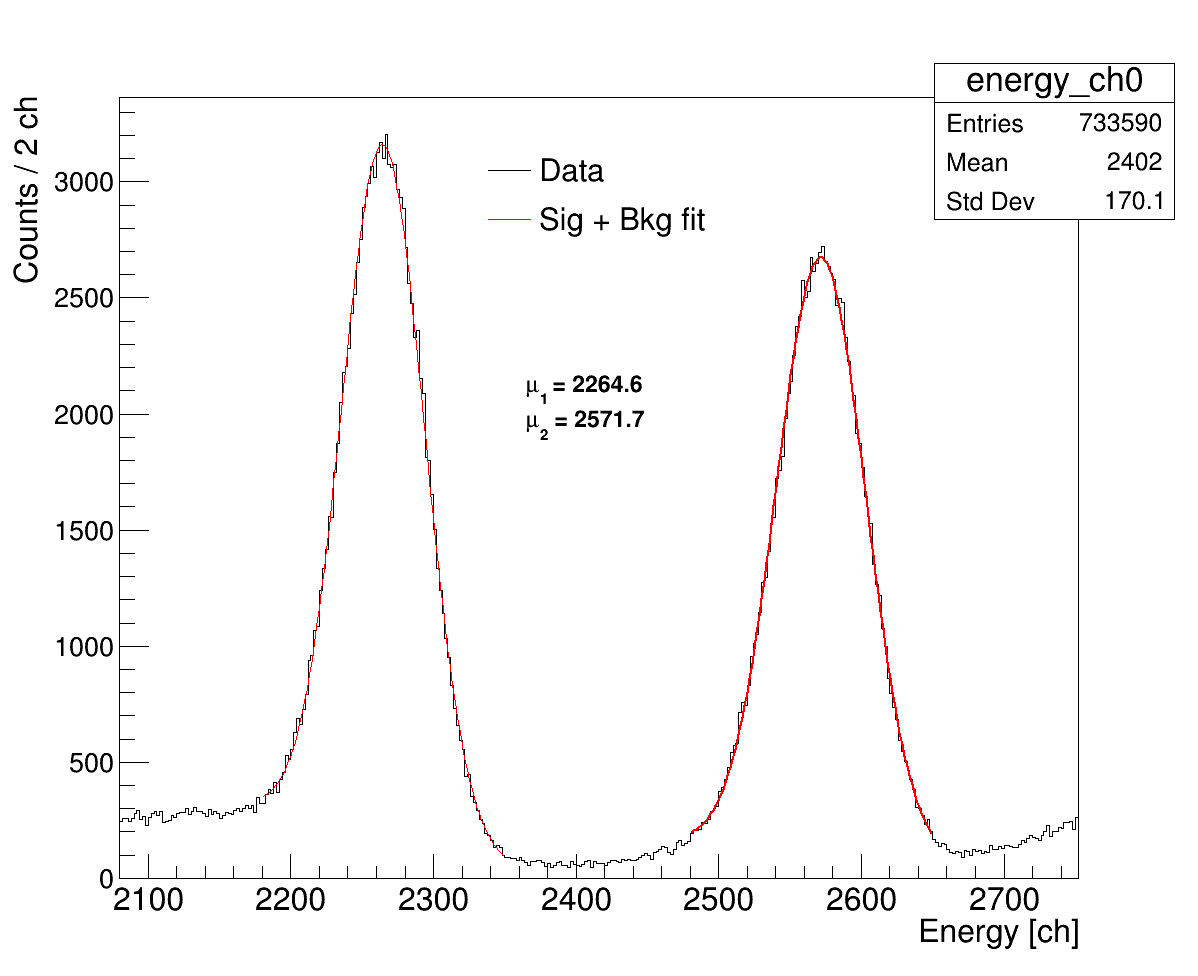
\includegraphics[width=0.9\textwidth]{Images/analysis/calibration/Co10_0.png} \label{fig:calib_Co_0} }
	\end{minipage}
	\begin{minipage}[]{0.5\linewidth}
	\centering
	\subfloat[][Channel 1.]{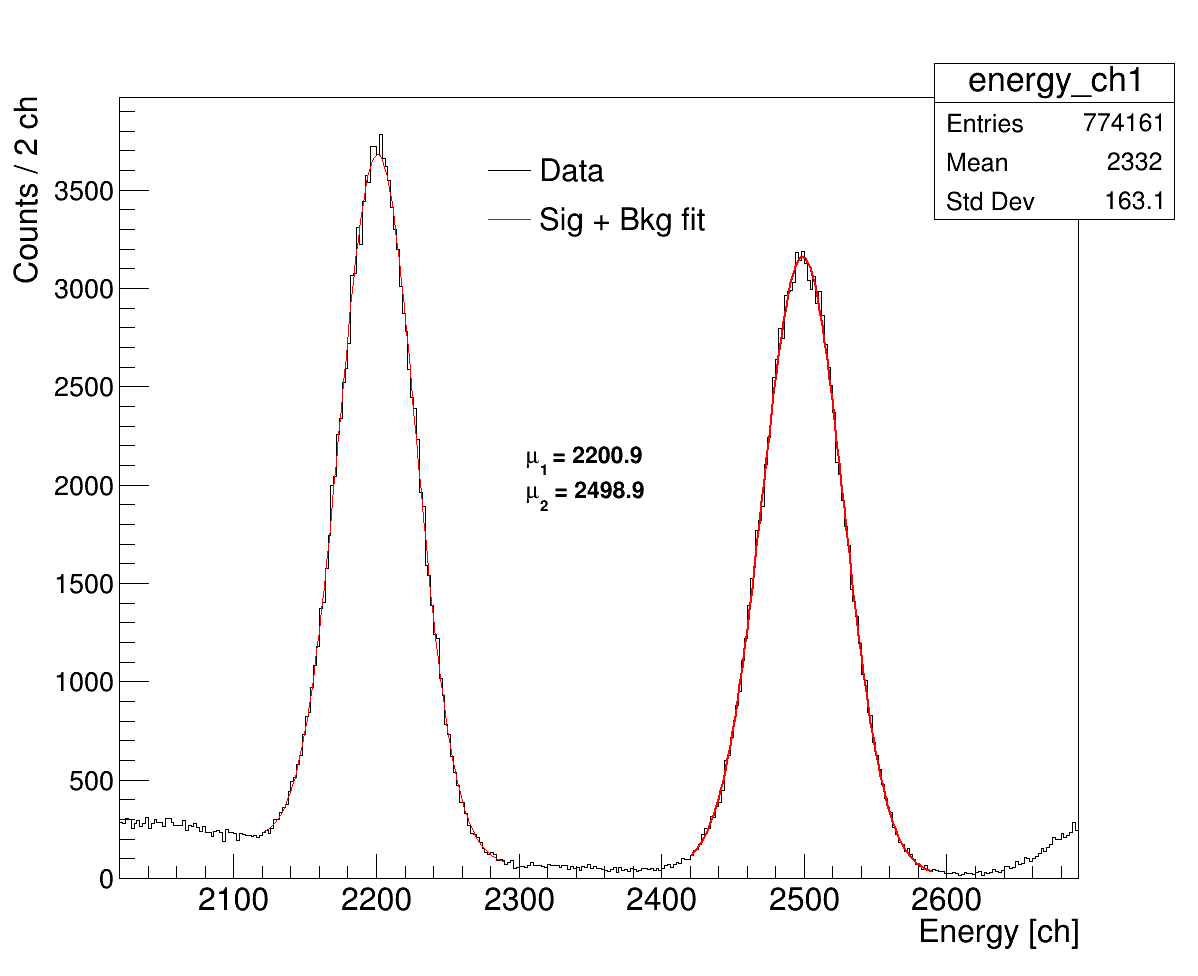
\includegraphics[width=0.9\textwidth]{Images/analysis/calibration/Co10_1.png}  \label{fig:calib_Co_1} }
	\end{minipage}
	\caption{\label{fig:calib_Co} Example of fits for the $^{60}$Co spectra at a distance of 10 cm.}
	\end{figure}


\begin{figure}[H]
	\begin{minipage}[c]{0.5\linewidth}
	\subfloat[][Channel 0.]{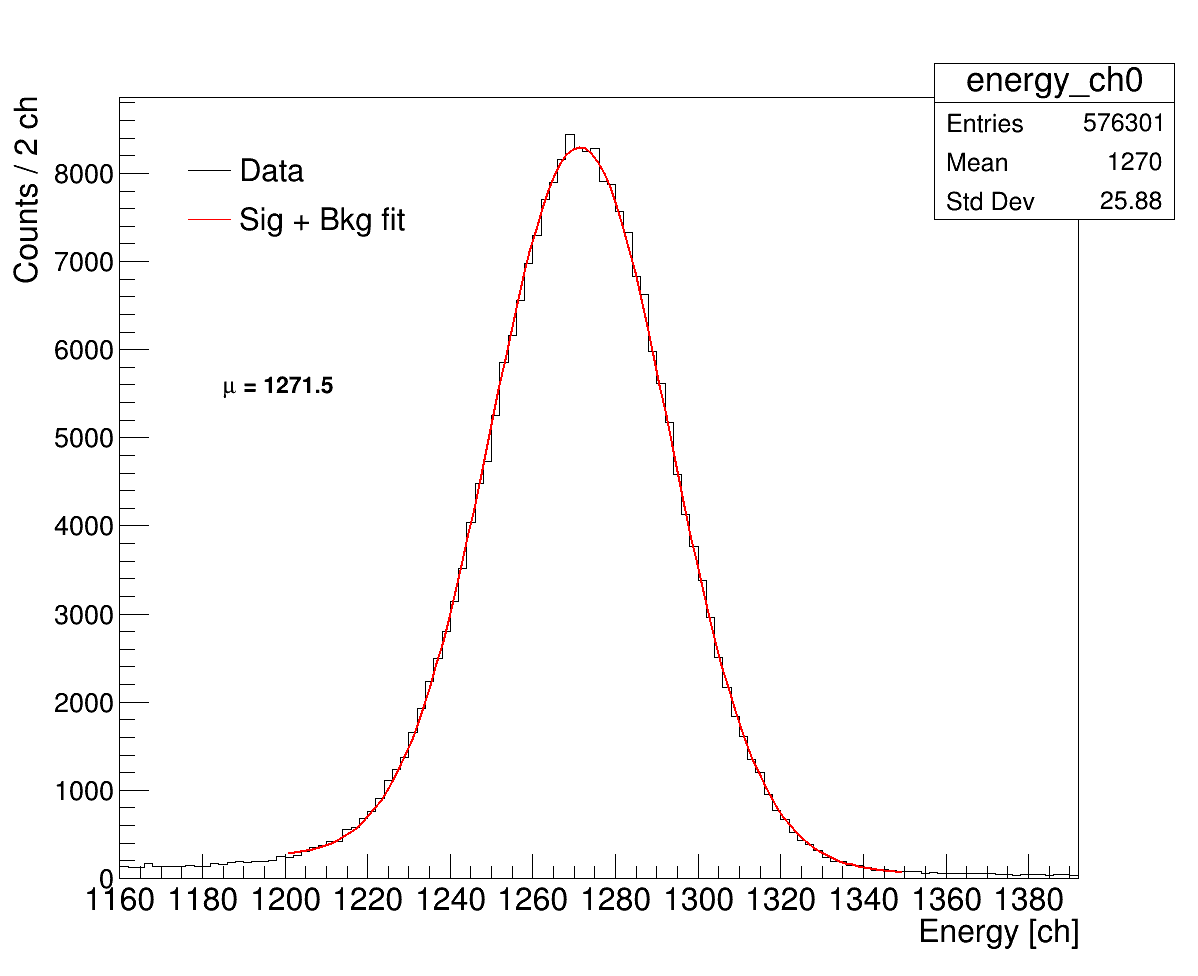
\includegraphics[width=0.9\textwidth]{Images/analysis/calibration/Cs10_0.png} \label{fig:calib_Cs_0} }
	\end{minipage}
	\begin{minipage}[]{0.5\linewidth}
	\centering
	\subfloat[][Channel 1.]{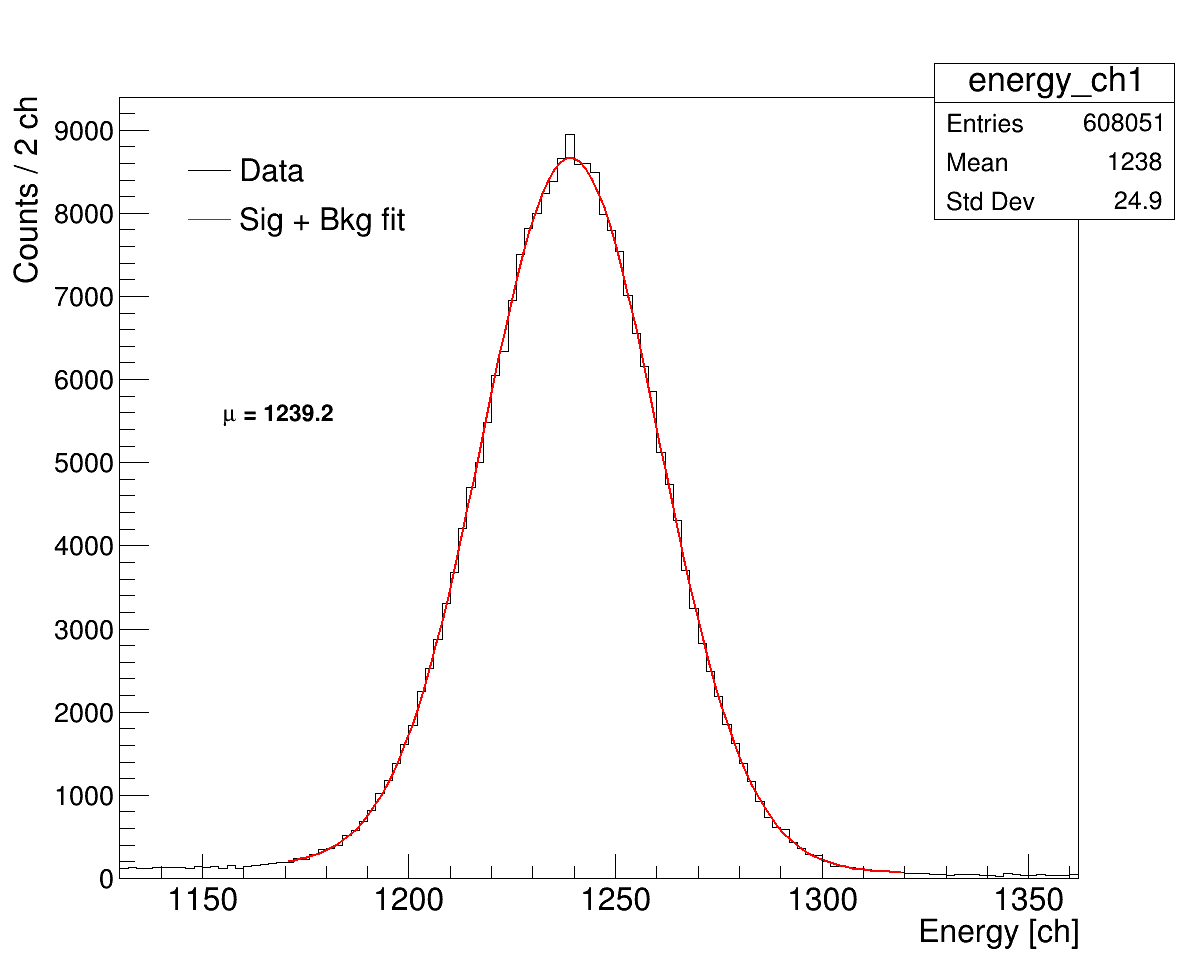
\includegraphics[width=0.9\textwidth]{Images/analysis/calibration/Cs10_1.png}  \label{fig:calib_Cs_1} }
	\end{minipage}
	\caption{\label{fig:calib_Cs} Example of fits for the $^{137}$Cs spectra at a distance of 10 cm.}
	\end{figure}
 

The relationship between energy and read-out channel is given by a linear interpolation of the reference values (fig. \ref{fig:cali}):

\begin{equation}
    E \; \left[keV\right] = m \cdot E \, \left[ch\right] + q
\end{equation}

The resulting values for the two channels are:
\begin{equation}
    \label{eq:calib}
    \begin{align}
        q_0 & = (6.68 \pm 0.05) \; keV \;\;\; 
        m_0   = (0.51785 \pm 0.00003) \; keV \\
        q_1 & = (1.80 \pm 0.04) \; keV \;\;\;
        m_1   = (0.53329 \pm 0.00002) \; keV	
    \end{align}
\end{equation}

\begin{figure}[H]
    \centering
    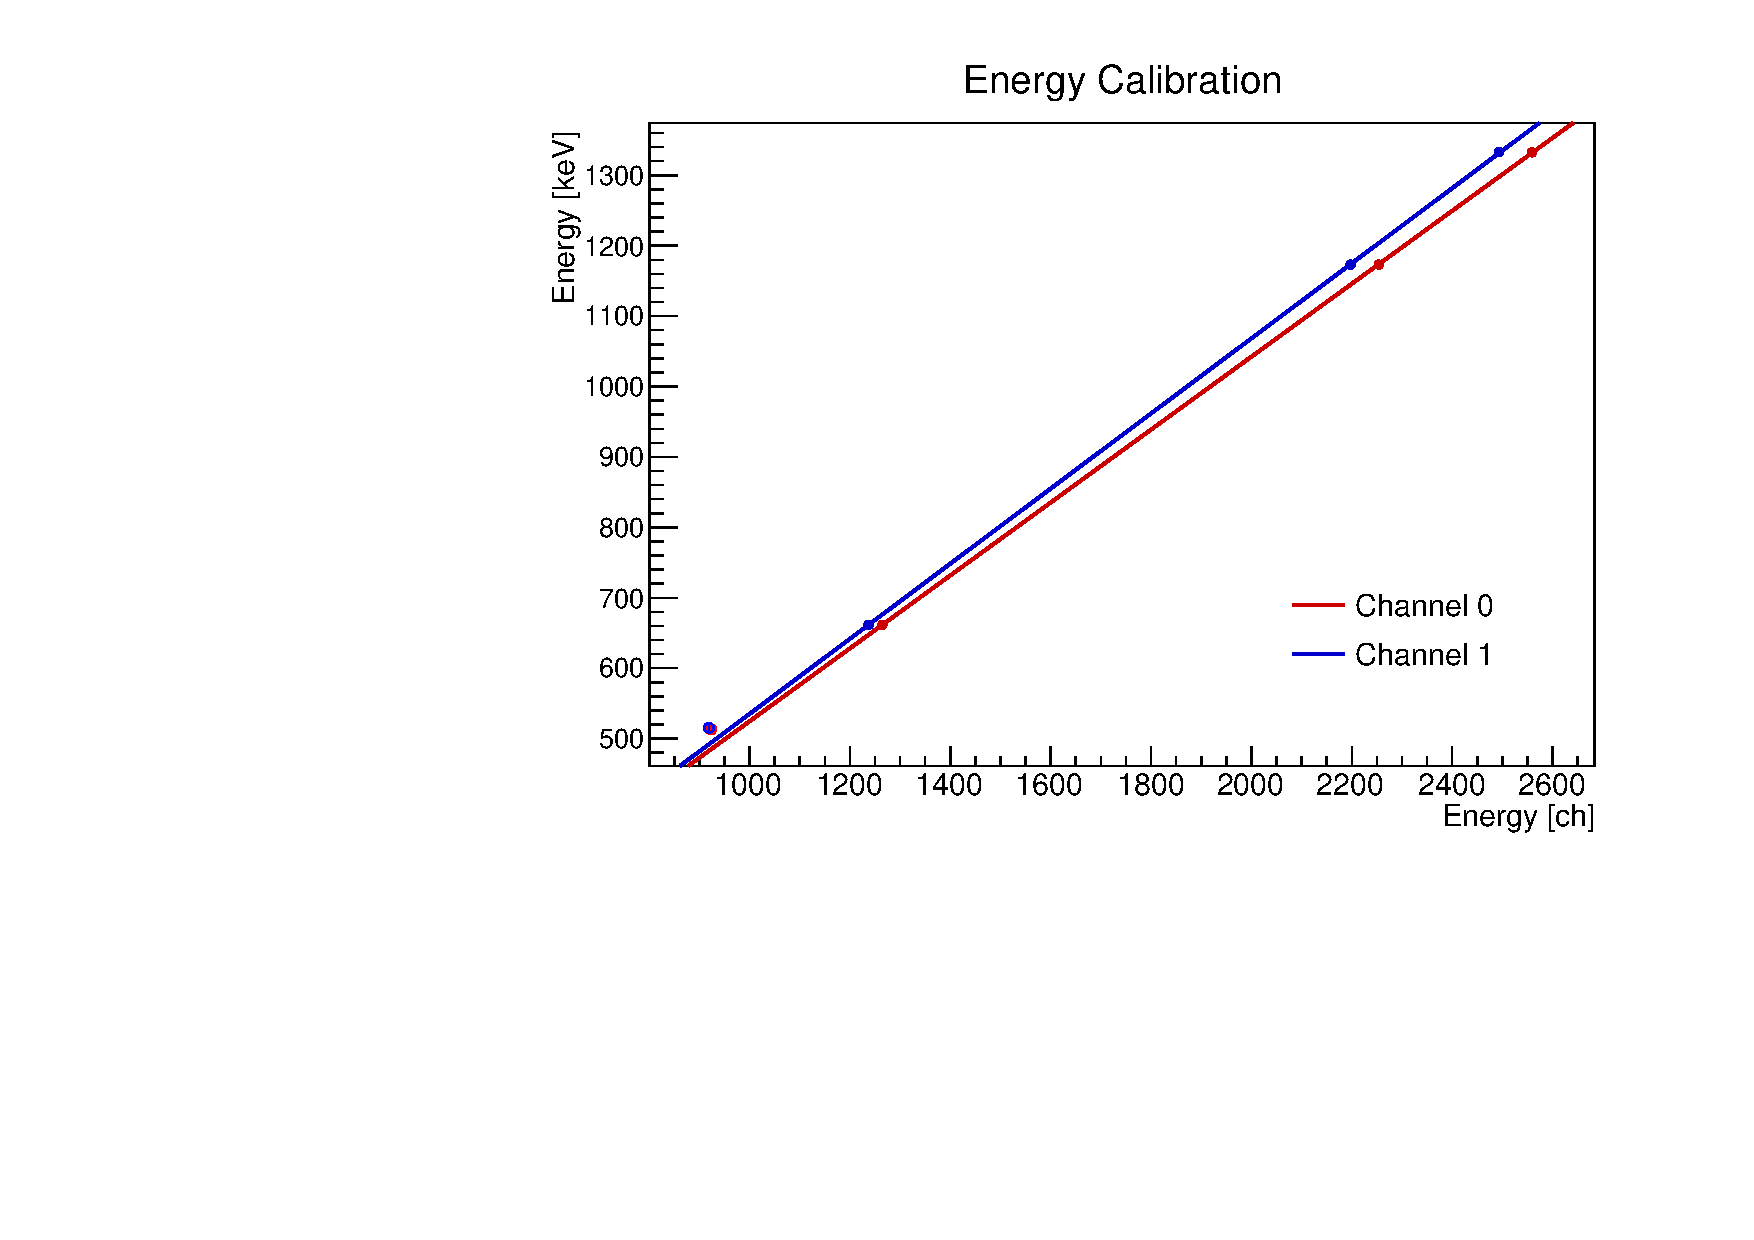
\includegraphics[scale=0.5]{Images/analysis/calibration/cali_2.pdf}
    \caption{Energy calibration of the detectors using $^{60}$Co and $^{137}$Cs, with channel 0 in blue and channel 1 in red. The first point represents for both channels the photopeak of $^{22}$Na at 511 keV, not used for the calibration.}
    \label{fig:cali}
\end{figure}


We then look at the photopeak of $^{22}Na$ at 511 keV. After finding the position as previously explained (fig. \ref{fig:calib_Na}), we can compare the theoretical value to the result expected using the calibration results in eq.\ref{eq:calib}. \\
The difference is of 5.3\% for channel 0 and 3.5\% and 1 respectively. This discrepancy can be due to the fact that the measurements using this source have been conducted on a different day and external factors influenced the calibration, e.g. the crystal temperature. \\
For consistency, we decide to continue using the calibration without $^{22}Na$.


\begin{figure}[H]
	\begin{minipage}[c]{0.5\linewidth}
	\subfloat[][Channel 0.]{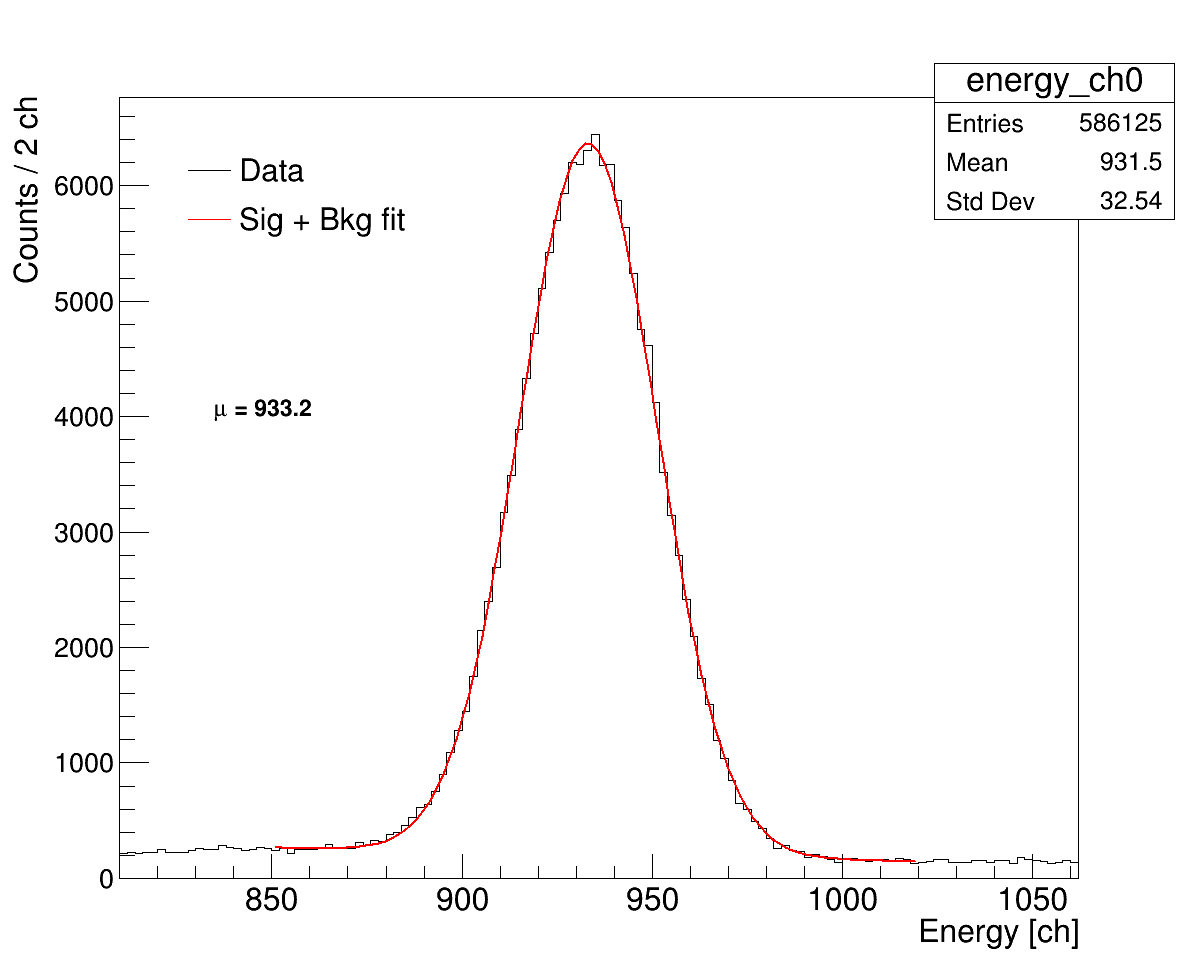
\includegraphics[width=0.9\textwidth]{Images/analysis/calibration/Na10_0.png} \label{fig:calib_Na_0} }
	\end{minipage}
	\begin{minipage}[]{0.5\linewidth}
	\centering
	\subfloat[][Channel 1.]{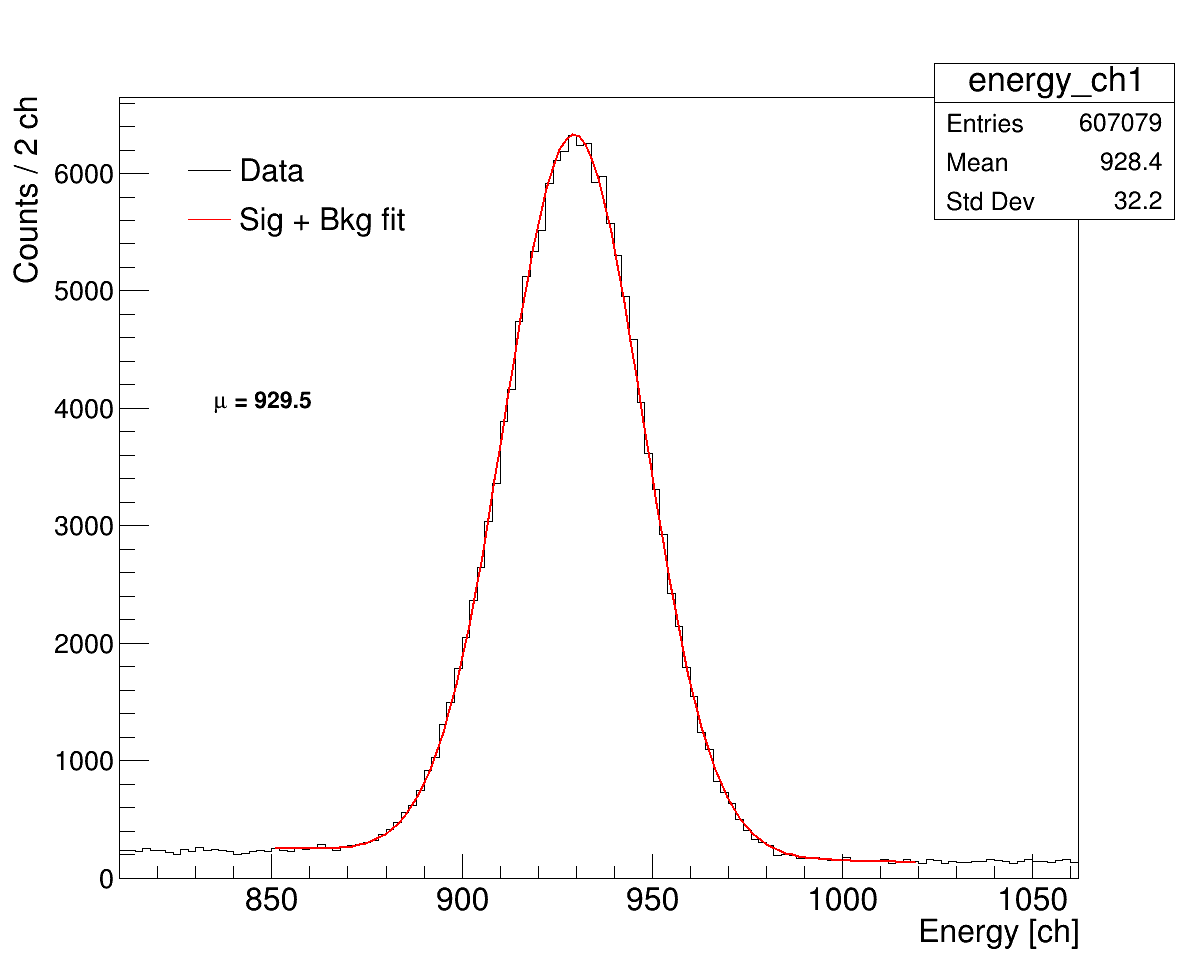
\includegraphics[width=0.9\textwidth]{Images/analysis/calibration/Na10_1.png}  \label{fig:calib_Na_1} }
	\end{minipage}
	\caption{\label{fig:calib_Na} Example of fits for the $^{22}$Na spectra at a distance of 10 cm.}
	\end{figure}







\section{Internal Background}
\label{sec:background}

A run without any radioactive source has been recorded to study the internal background of the detectors. The resulting spectrum for channel 0 is shown in fig. \ref{fig:bkg}.\\

$^{138}$La decays 66.4\% by electron capture to $^{138}$Ba, which emits a 1435.80 keV gamma-ray and the Ba X-rays. The remaining 33.6\% decays by $\beta$− emission to $^{138}$Ce, releasing a 788.74 keV gamma-ray. A bremmstrahlung continuum can be observed in the spectra extending to the beta end point at 255 keV. \\
Because the lanthanum atoms are decaying inside the detector, neither of the full-energy gamma-rays appear in the spectra as expected; both are summed – the 788.74 keV with its accompanying beta particles and the 1435.80 keV with the electron capture X-rays. At higher energies, there is evidence of low level alpha emitting contamination due to $^{227}$Ac contamination. 

\begin{figure}[h!]
\centering
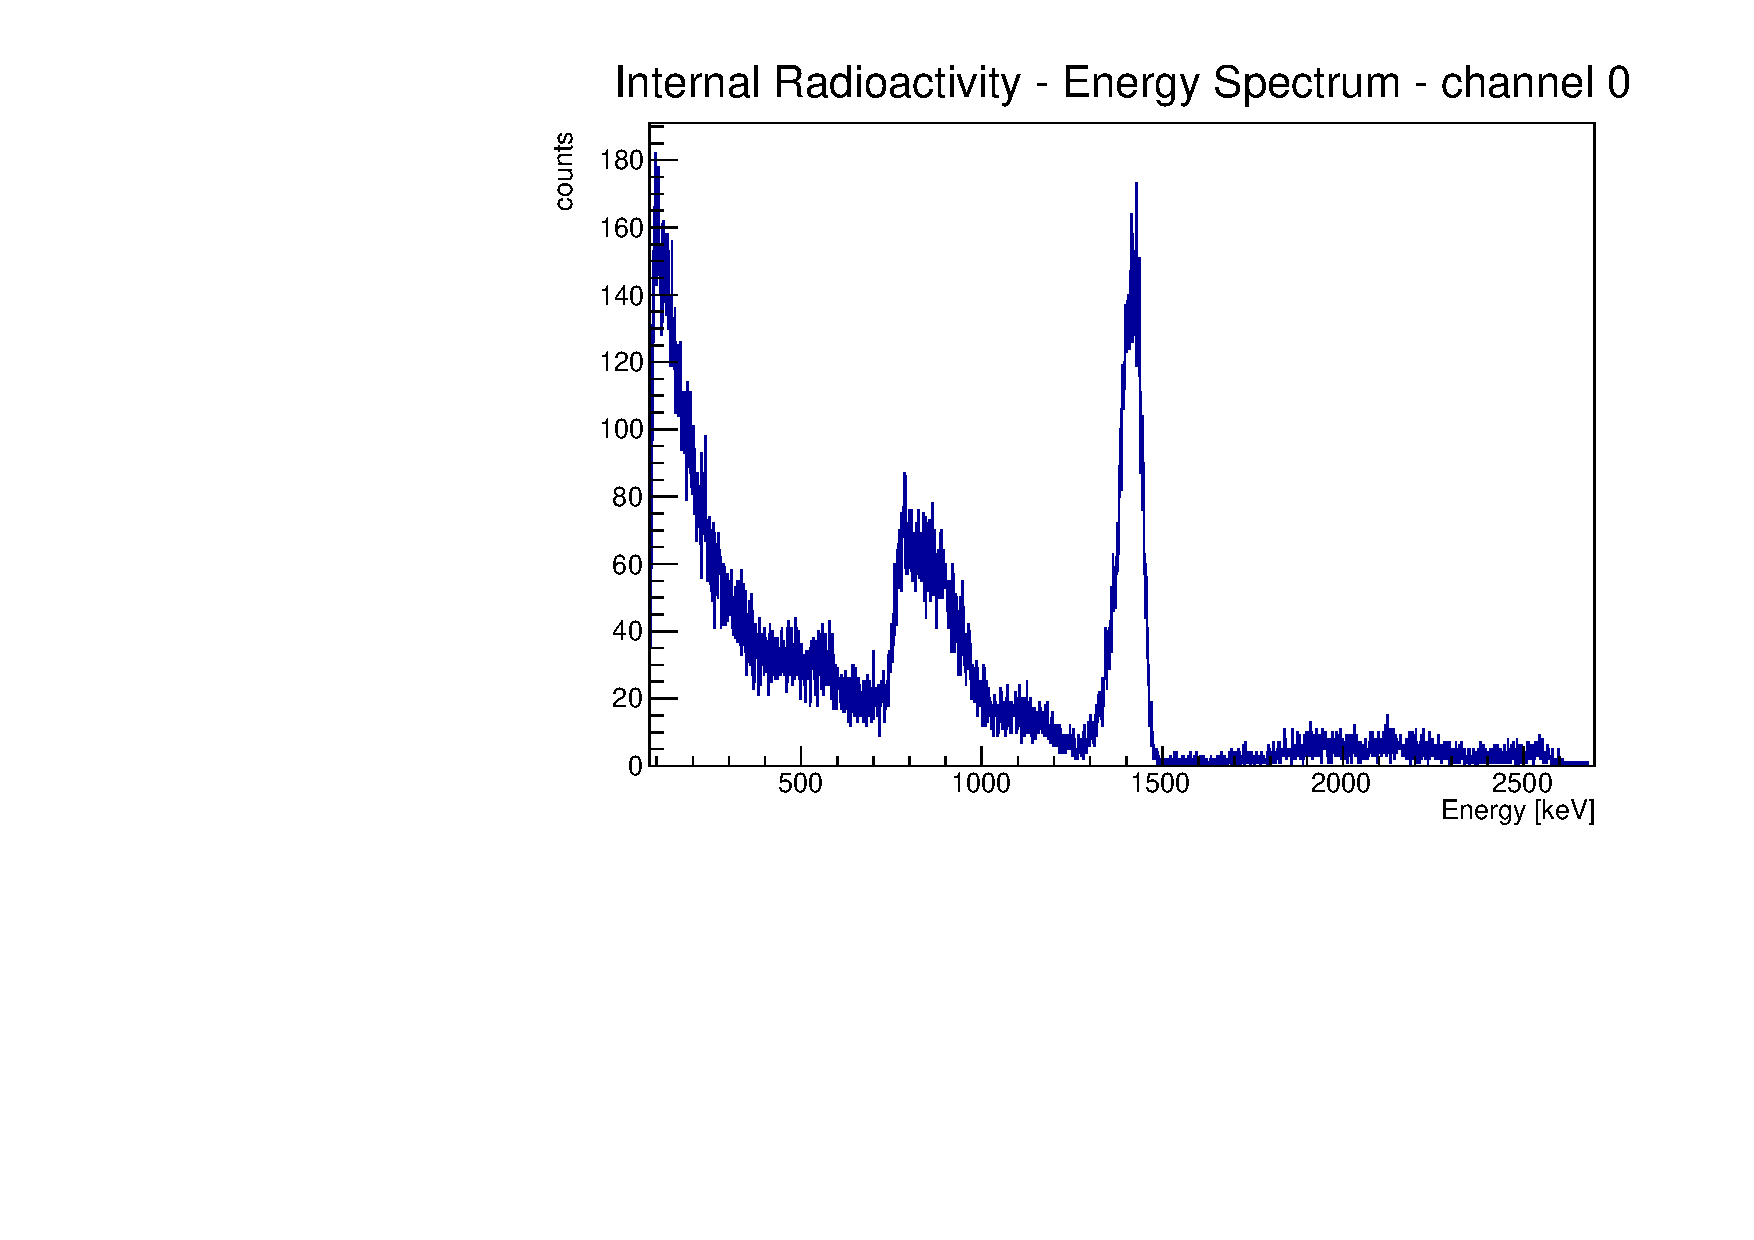
\includegraphics[width=0.6\textwidth]{Images/analysis/bkg/bg.pdf}
\caption{Background spectrum of the first detector. The three main features of the spectrum are clearly visible.}
\label{fig:bkg}
\end{figure}

\section{Resolution}
\label{sec:resolution}

We then characterize the resolution of the detector. To do so, we take the results of the photopeak fits of sec. \ref{sec:calibration} and compute the resolution as
\begin{equation}
    R = \cfrac{FWHM}{E_{photopeak}} \approx \cfrac{2.355 \; \sigma}{E_{photopeak}}
\end{equation}
The photopeaks considered are the one at 511 keV for $^{22}$Na, the one at 661.7 keV for $^{137}$Cs and the peaks at 1173.2 keV, 1332.5 keV and 2505.7 keV for $^{60}$Co, where the last peak represents the case in which both 1173.2 keV and 1332.5 keV gammas are detected by the same detector simultaneously, resulting in a peak with an energy corresponding to the sum of energies of the two gammas. These values are calculated for every distance and then averaged to obtain one single value for each energy. \\
In fig. \ref{fig:res} we can see the trend of the resolution values as a function of the energy; the values of the points are shown in tab. \ref{tab:res}.

\begin{figure}[H]
    \centering
    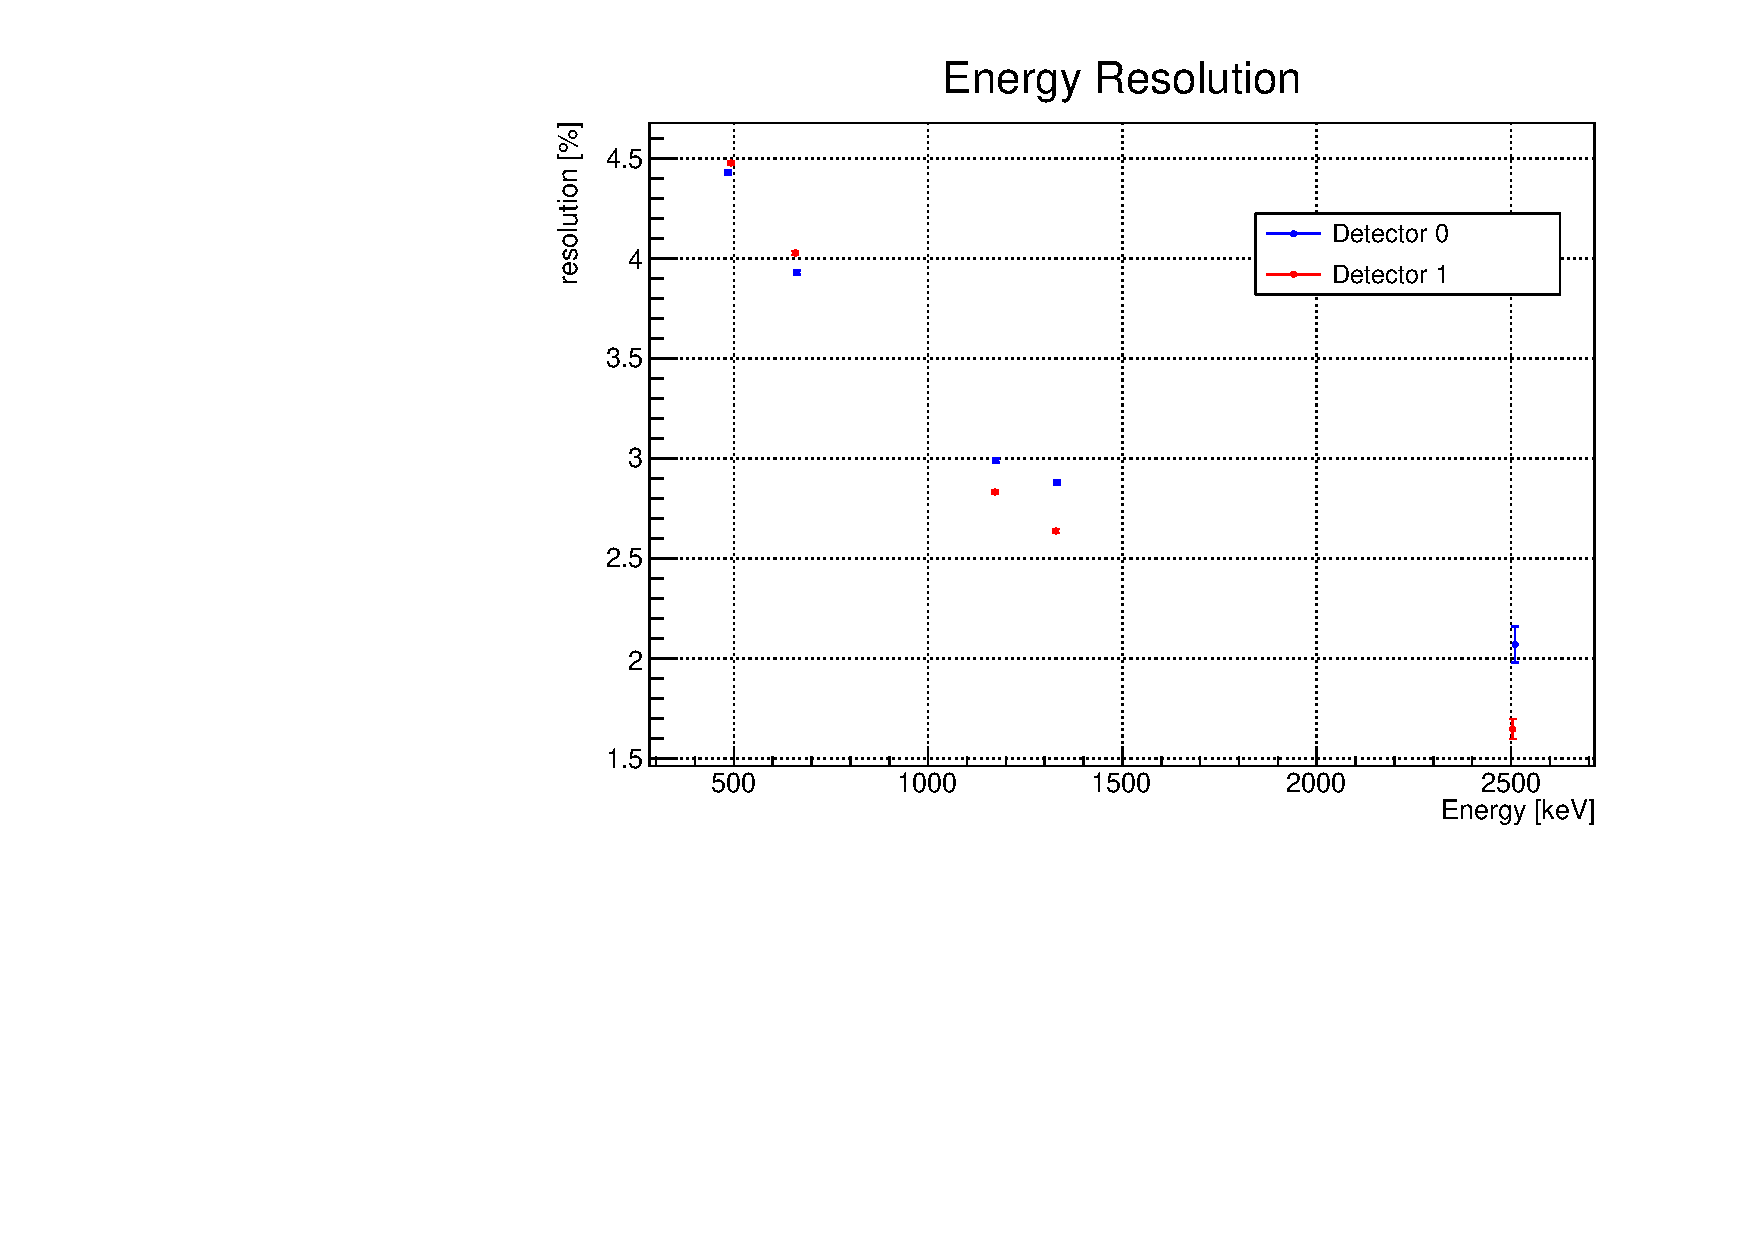
\includegraphics[scale=0.5]{Images/analysis/resolution/res.pdf}
    \caption{Energy resolution of the detectors, with detector 0 in blue and detector 1 in red.}
    \label{fig:res}
\end{figure}

\begin{table}[h]
    \begin{subtable}
        \centering
        \begin{tabular}{|c|c|c|c|}
         \hline
        E [keV] & $\sigma_{E} $ [keV] & res [\%] &$\sigma_{res}$ [\%]  \\
        \hline
        485.34 & 0.02 & 4.43 & 0.01 \\
        661.65 & 0.02 & 3.93 & 0.01 \\
        1173.84 &0.04& 2.99 & 0.01\\
        1331.70 & 0.04&2.88& 0.01\\
        2510.5 & 0.9&2.07& 0.09\\
        \hline
        \end{tabular}
    \end{subtable}
    \qquad
    \qquad
    \qquad
    \begin{subtable}
        \centering
        \begin{tabular}{|c|c|c|c|}
          \hline
        E [keV] & $\sigma_{E} $ [keV] & res [\%] &$\sigma_{res}$ [\%]  \\
        \hline
        493.29 & 0.02 &4.47 & 0.01 \\
        661.68 & 0.02 & 4.02 & 0.01 \\
        1173.64 &0.03& 2.83 & 0.01\\
        1332.17 & 0.03&2.63& 0.01\\
        2506.8 & 0.5&1.64& 0.05\\
        \hline
        \end{tabular}
     \end{subtable}
     \caption{Values of resolution at different energies for detector 0 and 1 respectively.}
     \label{tab:res}
\end{table}

We can then fit the values for the resolution an FWHM to some commonly used functions \cite{gilmore_2008}, shown respectively in the first and second table of tab. \ref{table:Funzioni}.
The results of said fits are shown in fig. \ref{fig:resolution} for the resolution and in fig. \ref{fig:FWHM} for the FWHM, while the values of the parameters of the fit are shown in tab. \ref{table:fit_res0}-\ref{table:fit_FWHM1}.

\begin{table}[h]
    \begin{subtable}
        \centering
        \begin{tabular}{|c|c|}
        \hline
        \multicolumn{2}{|c|}{Function to fit the resolution}\\
        \hline
        F1 & $ res = \frac{a}{E} + b$\\
        F2 & $ res = \frac{a}{E} + b + c \cdot E $ \\
        F3 & $ res = \frac{a}{E} + \frac{b}{E^{3/2}}$\\
        F4 & $ res = \sqrt{\frac{a^2}{E^2}+\frac{b^2}{E}}$\\
        F5 & $ res = \sqrt{\frac{a^2}{E^2}+\frac{b^2}{E}+c^2}$\\
        \hline
        \end{tabular}
    \end{subtable}
    \qquad
    \qquad
    \qquad
    \begin{subtable}
        \centering
        \begin{tabular}{|c|c|}
        \hline
        \multicolumn{2}{|c|}{Functions to fit the FWHM}\\
        \hline
        G1 & $ FWHM = a + b \cdot E$\\
        G2 & $ FWHM = a+ b \cdot E + c \cdot E^{2} $ \\
        G3 & $ FWHM = a + \frac{b}{\sqrt{E}}$\\
        G4 & $ FWHM = \sqrt{a^2+b^2 E} $\\
        G5 & $ FWHM = \sqrt{a^2+b^2E+c^2E^2}$\\
       \hline
        \end{tabular}
     \end{subtable}
     \caption{Functions used for fitting the energy resolution and the FWHM, respectively.}
     \label{table:Funzioni}
\end{table}

\begin{figure}[H]
	\begin{minipage}[c]{0.5\linewidth}
	\subfloat[][Channel 0.]{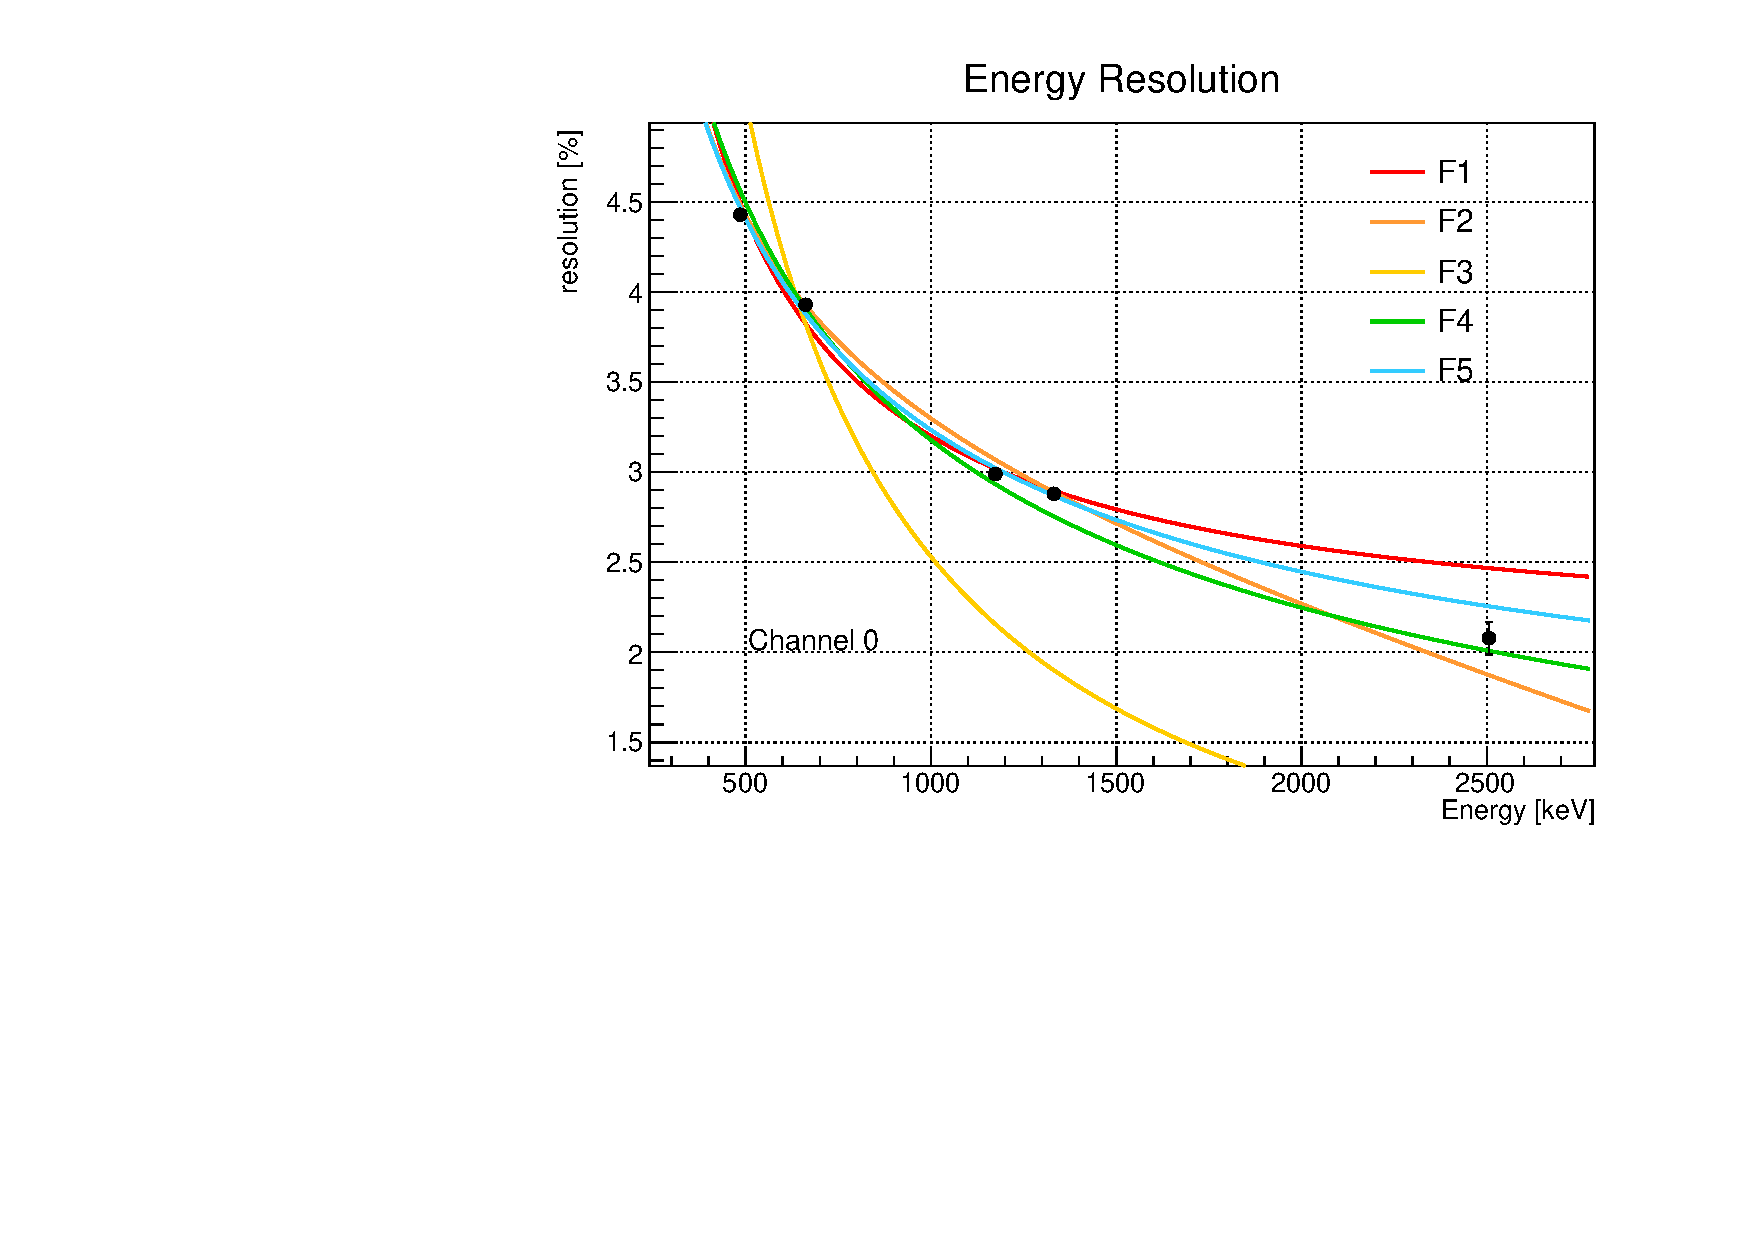
\includegraphics[width=0.9\textwidth]{Images/analysis/resolution/res0_fit.pdf} \label{fig:res0} }
	\end{minipage}
	\begin{minipage}[]{0.5\linewidth}
	\centering
	\subfloat[][Channel 1.]{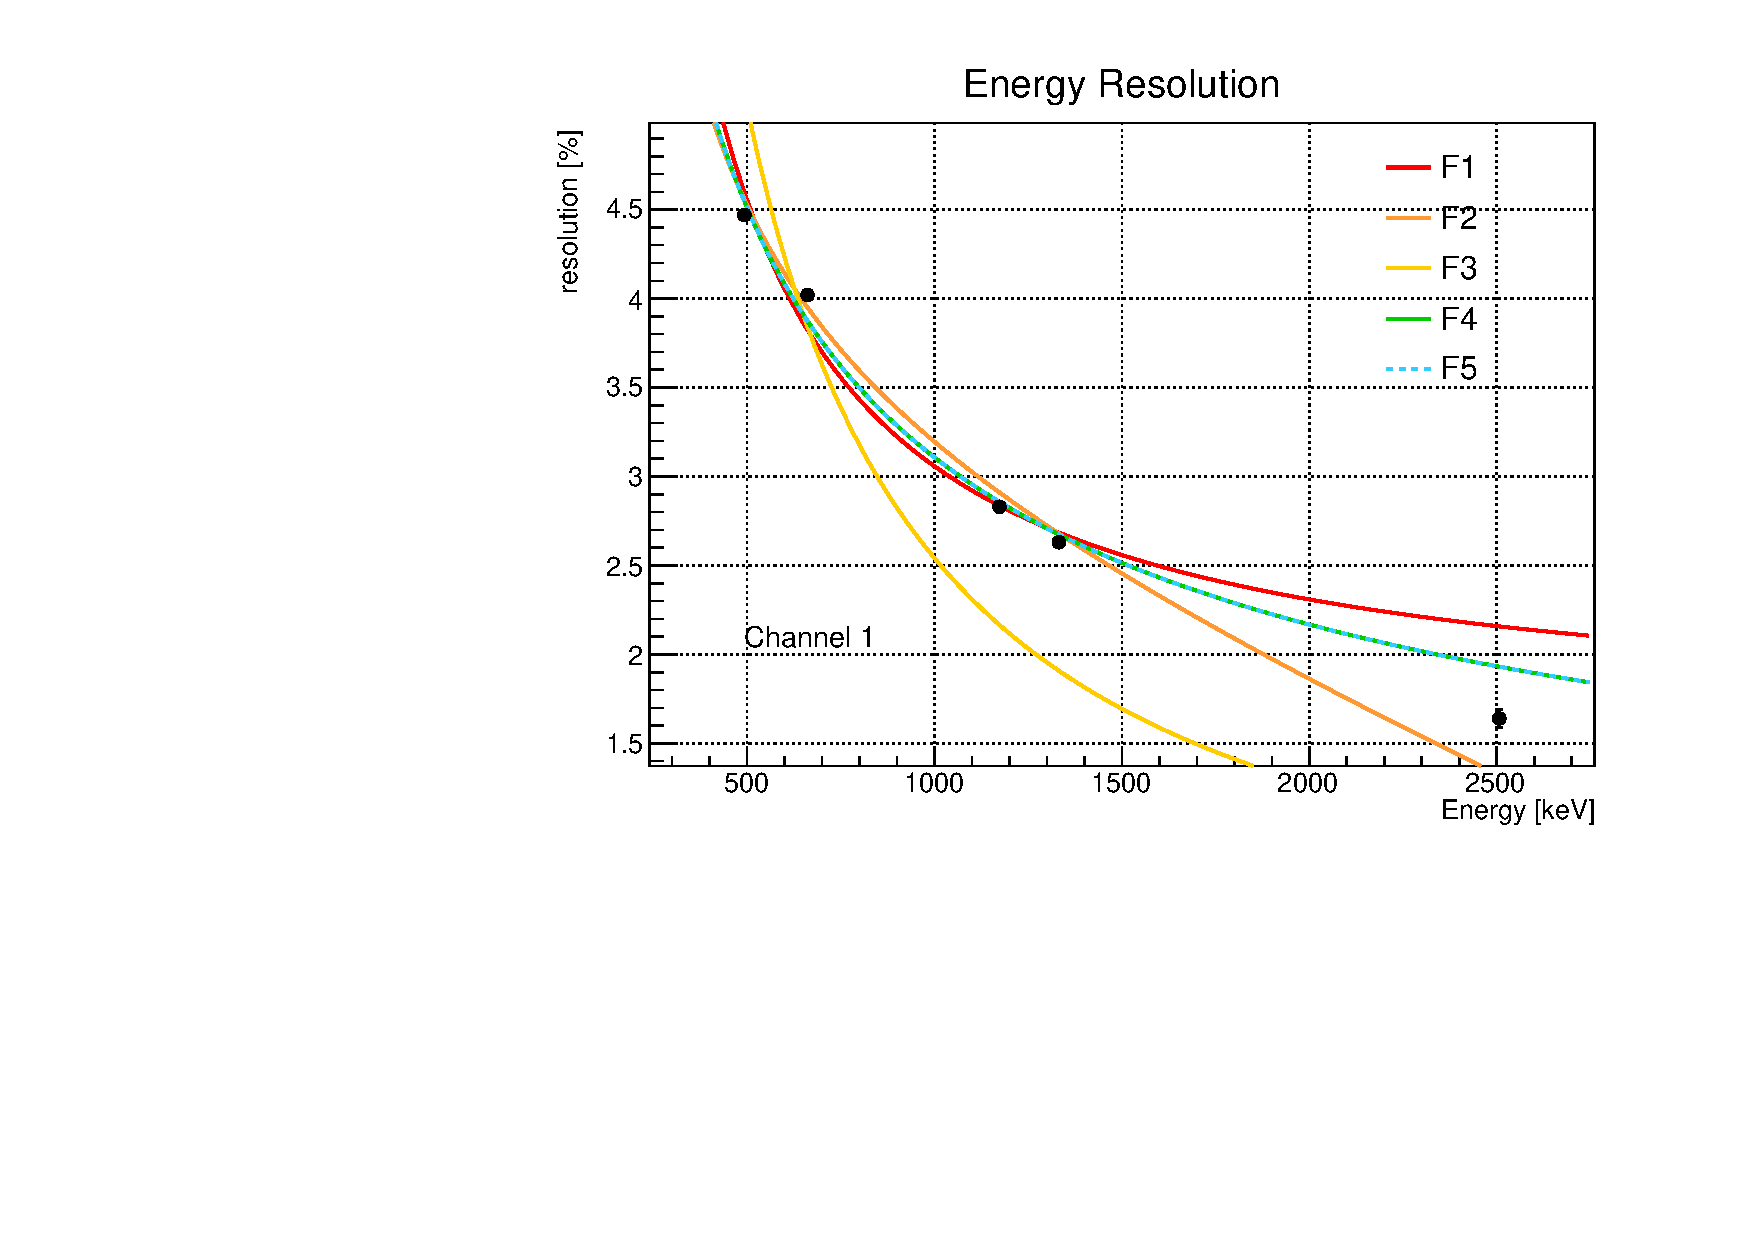
\includegraphics[width=0.9\textwidth]{Images/analysis/resolution/res1_fit.pdf}  \label{fig:res1} }
	\end{minipage}
	\caption{Fit of the energy resolution through the functions in the first table of tab.\ref{table:Funzioni}.}
    \label{fig:resolution}
	\end{figure}

\begin{figure}[H]
	\begin{minipage}[c]{0.5\linewidth}
	\subfloat[][Channel 0.]{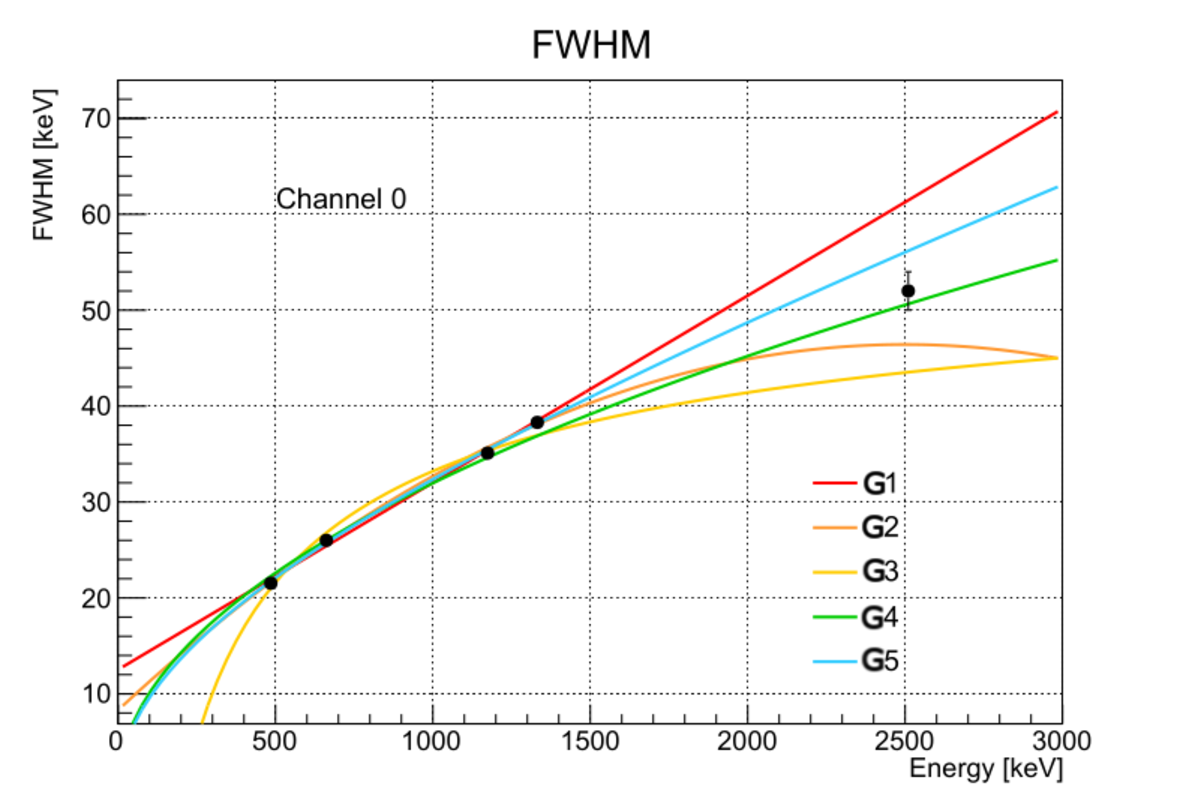
\includegraphics[width=0.9\textwidth]{Images/analysis/resolution/FWHM0.pdf} \label{fig:FWHM0} }
	\end{minipage}
	\begin{minipage}[]{0.5\linewidth}
	\centering
	\subfloat[][Channel 1.]{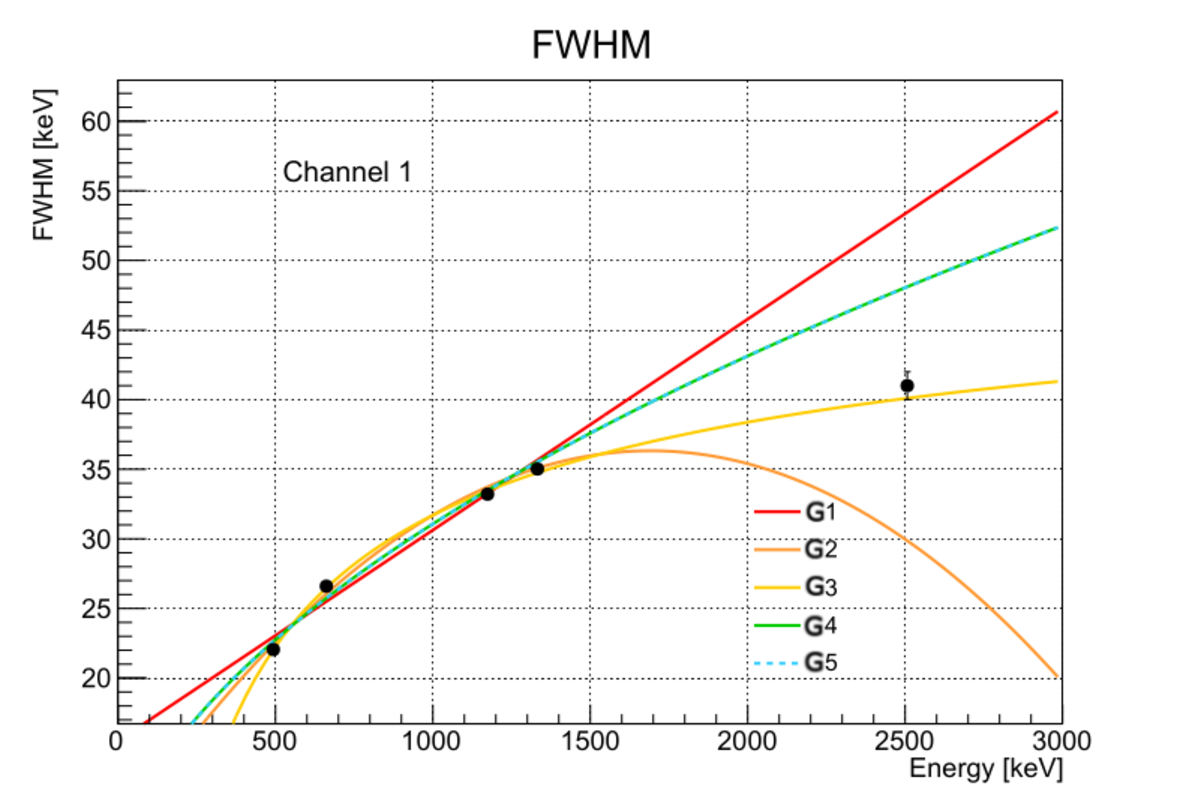
\includegraphics[width=0.9\textwidth]{Images/analysis/resolution/FWHM1.pdf}  \label{fig:FWHM1} }
	\end{minipage}
	\caption{Fit of the FWHM through the functions in the second table of tab.\ref{table:Funzioni}.}
    \label{fig:FWHM}
	\end{figure}

\begin{table}[ht]
    \centering
    \begin{tabular}{|c|c|c|c|c|}
    \hline
     & a & b & c & $\chi /dof$  \\
    \hline
    F1 & $(1220 \pm 9)$ keV & $(1.98 \pm 0.01)$ & - & 183.6/3 \\
    F2 & $(8.2 \pm 0.4) \times 10^2$ keV & $(3.1 \pm 0.1)$ & $(-0.62 \pm 0.05)10^{-3}$ keV$^{-1}$ & 52.01/2 \\
    F3 & $(2 \pm 1) \times 10^3$ keV & $(1 \pm 1)10^3$ keV$^{3/2}$ & - & 22950/3 \\
    F4 & $(0.0 \pm 0.6)$ keV & $(100.5 \pm 0.1)$ keV$^{1/2}$ & - & 370.5/3 \\
    F5 & $(0 \pm 2)$ keV & $(94.6 \pm 0.4)$ keV$^{1/2}$ & $(1.23 \pm 0.03)$ & 56.34/2 \\
    \hline
    \end{tabular}
    \caption{Parameters of the functions fitting energy resolution for detector 0.}
    \label{table:fit_res0}
\end{table}

\begin{table}[ht]
    \centering
    \begin{tabular}{|c|c|c|c|c|}
    \hline
     & a & b & c & $\chi /dof$  \\
    \hline
    F1 & $(15.0 \pm 0.1) \times 10^2$ keV & $(1.56 \pm 0.01)$ & - & 681.90/3 \\
    F2 & $(8.9 \pm 0.3) \times 10^2$ keV & $(3.2 \pm 0.1)$ & $(-0.89 \pm 0.04) \times 10^{-3}$ keV$^{-1}$ & 209.4/2 \\
    F3 & $(2 \pm 0.5) \times 10^3$ keV & $(0.8 \pm 0.5)10^4$ keV$^{3/2}$ & - & 14760/3 \\
    F4 & $(7.2 \pm 0.4) \times 10^2$ keV & $(95.6 \pm 0.4)$ keV$^{1/2}$ & - & 334.8/3 \\
    F5 & $(7.2 \pm 0.3) \times 10^2$ keV & $(94.6 \pm 0.4)$ keV$^{1/2}$ & $(0.00 \pm 0.01)$ & 334.8/2\\
    \hline
    \end{tabular}
    \caption{Parameters of the functions fitting energy resolution for detector 1, note that the results for F4 and F5 are the same.}
    \label{table:fit_res1}
\end{table}

\begin{table}[ht]
    \centering
    \begin{tabular}{|c|c|c|c|c|}
    \hline
     & a & b & c & $\chi /dof$  \\
    \hline
    G1 & $(12.52 \pm 0.08)$ keV & $(0.0195 \pm 0.0001)$ & - & 251.6/3 \\
    G2 & $(8.3 \pm 0.3)$ keV & $(0.0305 \pm 0.0008)$ & $(-6.1 \pm 0.5) \times 10^{-6}$ keV $^{-1}$ & 68.81/2 \\
    G3 & $(61.2 \pm 0.2)$ keV & $(-885 \pm 5)$ keV$^{3/2}$ & - & 560.8/3 \\
    G4 & $(0.00 \pm 0.01)$ keV & $(1.011 \pm 0.001)$ keV$^{1/2}$ & - & 440.1/3 \\
    G5 & $(0.000 \pm 0.004)$ keV & $(0.953 \pm 0.003)$ keV$^{1/2}$ & $(0.0118 \pm 0.0003)$ & 71.16/2 \\
    \hline
    \end{tabular}
    \caption{Parameters of the functions fitting FWHM for detector 0.}
    \label{table:fit_FWHM0}
\end{table}

\begin{table}[H]
    \centering
    \begin{tabular}{|c|c|c|c|c|}
    \hline
     & a & b & c & $\chi /dof$  \\
    \hline
    G1 & $(15.48 \pm 0.07)$ keV & $(0.01515 \pm 0.00009)$ & - & 1480/3 \\
    G2 & $(8.6 \pm 0.2)$ keV & $(0.0328 \pm 0.0006)$ & $(-9.7 \pm 0.3) \times 10^{-6}$ keV$^{-1}$ & 450.7/2 \\
    G3 & $(54.5 \pm 0.2)$ keV & $(-721 \pm 4)$ keV$^{3/2}$ & - & 31/3 \\
    G4 & $(8.4 \pm 0.2) \times 10^2$ keV & $(0.946 \pm 0.003)$ keV$^{1/2}$ & - & 773.9/3 \\
    G5 & $(8.4 \pm 0.2) \times 10^2$ keV & $(0.946 \pm 0.003)$ keV$^{1/2}$ & $(0.00 \pm 0.02)10^{-3}$ & 773.9/2\\
    \hline
    \end{tabular}
    \caption{Parameters of the functions fitting FWHM for detector 1, note that the results for G4 and G5 are the same.}
    \label{table:fit_FWHM1}
\end{table}

\section{Timing Performances}
\label{sec:timing}

We now study the timing performances and coincidences of the two detectors. To do so, we first compute the difference between the recorded timing of each event of a channel with the timing of all the events from the other, and then take into account only the pair of events with the smallest time difference. Lastly, we plot this difference in a histogram in order to obtain the spectra of the time differences between events read from the two detectors. \\
For this analysis we use $^{22}$Na, as the two gammas produced in the decay are emitted simultaneously in opposite direction: thus, if a detector sees one gamma, we expect the other to detect one as well. \\

The spectrum in fig.\ref{fig:timing} shows that we have a constant distribution of time differences, which represents the non-correlated events background, with a peak around the zero representing the events in coincidence. Since the time difference for event in coincidence should be zero, we can consider the width of the peak as the timing resolution of the detectors. \\
The histogram is fit with eq.\ref{eq:fit_time}, where C is the position of the highest bin, since the peak clearly decays exponentially. 

\begin{equation}\label{eq:fit_time}
    f(x)= 
\begin{cases}
    a+b \cdot e^{\frac{(x-C)+d}{e}}& \text{if } x<C\\
    a+b \cdot e^{\frac{-(x-C)+d}{e}}              & \text{if } x \geq C
\end{cases}
\end{equation} 

\begin{figure}[H]
    \centering
    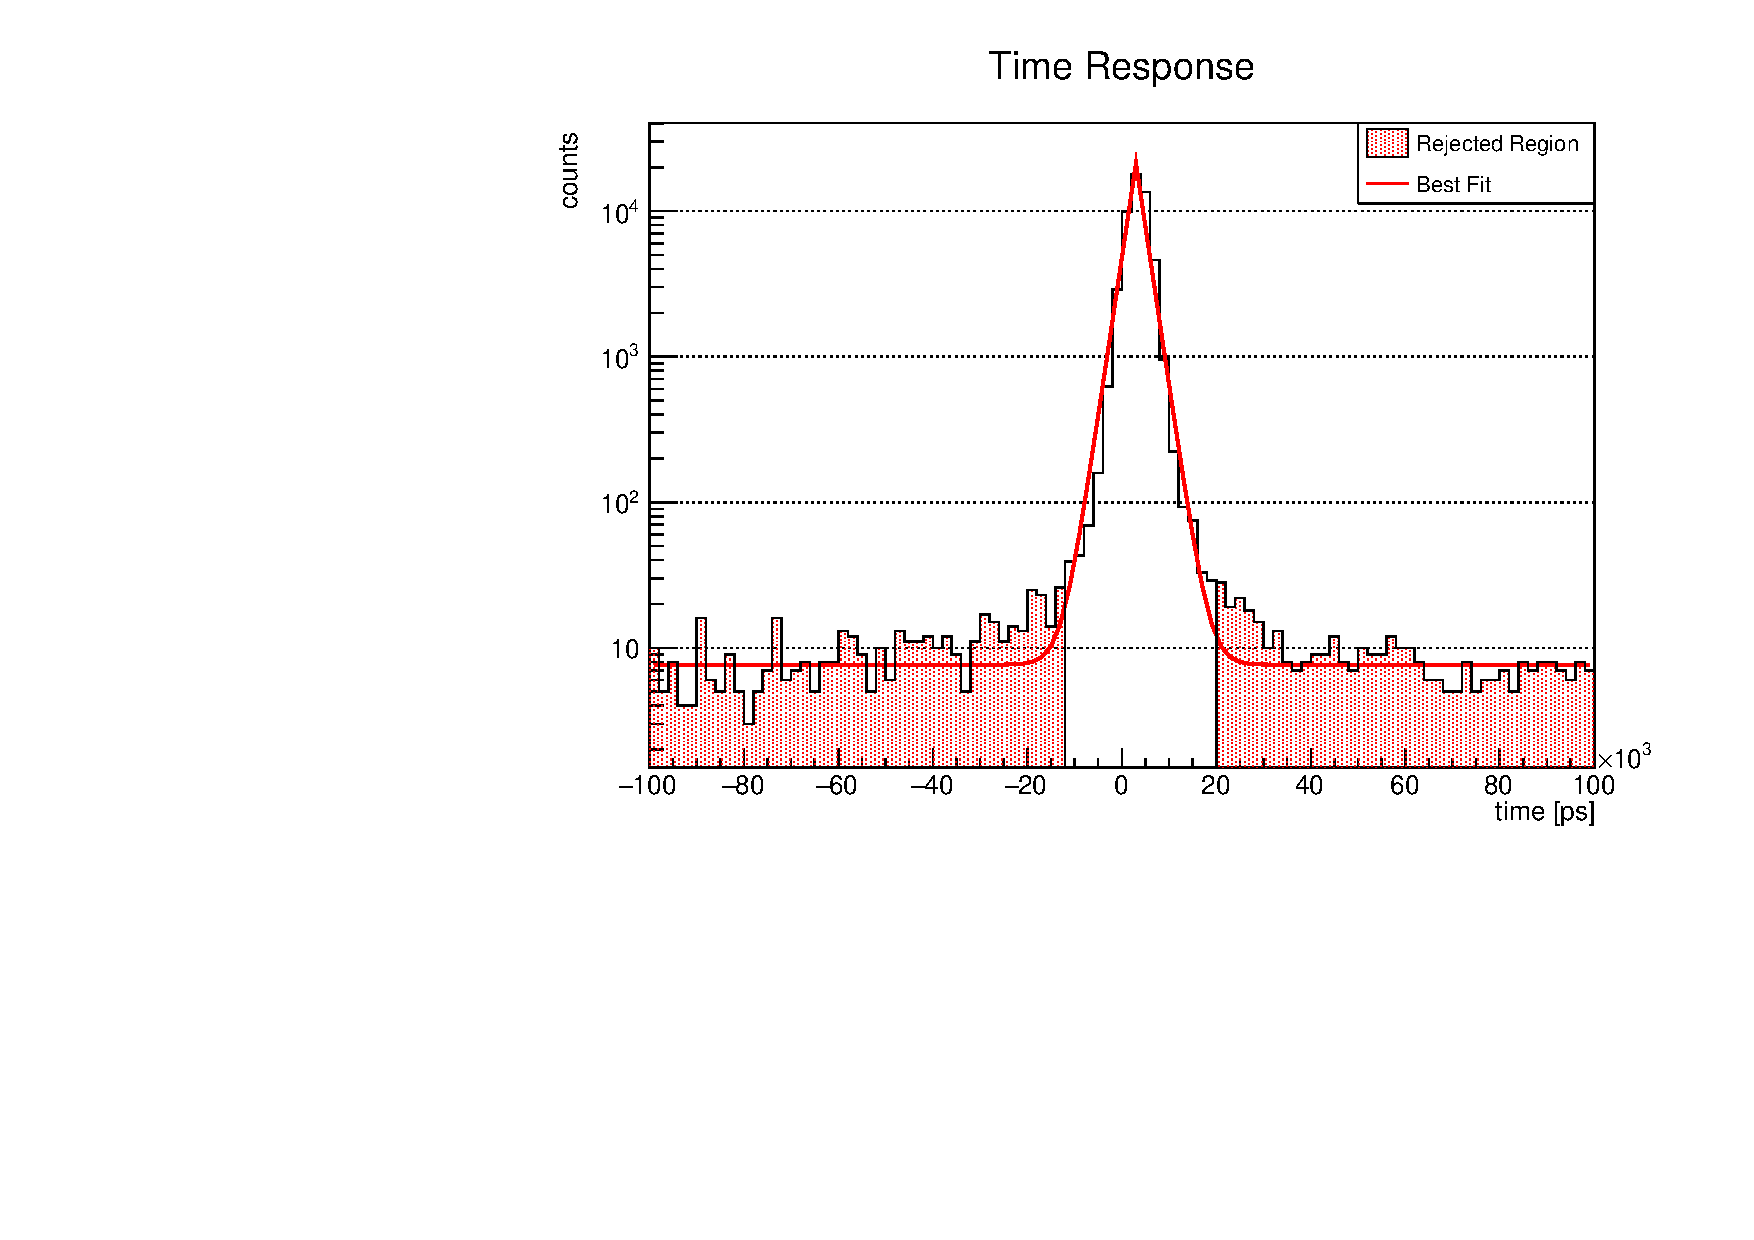
\includegraphics[scale=0.5]{Images/analysis/timing/time_response.pdf}
    \caption{Spectra of the time response of the detector for the source of $^{22}$Na. The best fit is shown as the red line, while the unrelated events region is shaded in red.}
    \label{fig:timing}
\end{figure}
 
Since the  peak is not gaussian, we decide to consider the width of the distribution as the difference between the two points where the derivative of the fit is equal to $e^{-6}$, $t_{0}^{\pm}$, shown in tab. \ref{table:t0}. The choice of $e^{-6}$ holds no particular physical meaning, but has been decided arbitrarily to have a reference value close enough to zero that provided reasonable results. In fig.\ref{fig:timing} the rejected region, corresponding to unrelated events, is highlighted along with the fitting function.

\begin{table}[ht]
    \centering
    \begin{tabular}{|c|c|c|c|c|}
    \hline
     & \multicolumn{2}{|c|}{Channel 0} & \multicolumn{2}{|c|}{Channel 1}\\
    \hline
    Source distance& $t_{0}^{-}$ [ns] & $t_{0}^{+}$ [ns] & $t_{0}^{-}$ [ns] & $t_{0}^{+}$ [ns] \\
    \hline
    10 cm& -13.7 & 19.7 & -17.7 & 15.7 \\
    15 cm& -13.1 & 19.1 & -17.1 & 15.1 \\
    20 cm& -13.3 & 19.3 & -17.3 & 15.3 \\
    Mean&  -13.4& 19.4& -17.4 & 15.4 \\
    \hline
    \end{tabular}
    \caption{Values that contain the coincidence region in the timing spectra, for detector 0 and 1, at different distances of the source. The last row shows the average between the different distances.}
    \label{table:t0}
\end{table}

Taking the average value of $t_{0}^{\pm}$, for both channels, we can estimate the width of the region, resulting in $ \Delta t_{ch0}=16.4$ ns and $\Delta t_{ch1}=16.4$ ns. We will thus considere a pair of events from channel 0 and 1 in coincidence if the time difference between them was less than 16 ns. \\
Note that the interval is the same for both detector, meaning they have the same time resolution as expected, but the ranges of coincindence shift from one channel to the other. This may be due to the fact that the source could have been placed not exactly in the center.

The effect of imposing the timing coincidence is shown in figure \ref{fig:T_effect_Na} and \ref{fig:T_effect_Co}, where in the subfigures \ref{fig:Na_ee} and \ref{fig:Co_ee} we can see the corresponding energies between the events in the two channel that have the smallest timing difference. We can observe, that without imposing the timing coincidence condition, we see correlation between peaks happening simoultaneously, but also with other energy values that are not necessarily in coincidence, as the one of the intrinsic radioactivity of the detector, around 1400 keV, or the one at 1275 keV for $^{22}$Na.
When we impose the timing coincidences, fig. \ref{fig:Na_ee_coinc} and \ref{fig:Co_ee_coinc}, we see that the only correlation left is only the one corresponding to events happening simultaneously, the two peaks at 511 keV for $^{22}$Na and the peaks at 1332 keV and 1173 keV for $^{60}$Co. So when one detector sees a peak the other sees the other peak.
\begin{figure}[H]
	\begin{minipage}[c]{0.5\linewidth}
	\subfloat[][No timing coincidence.]{\includegraphics[width=0.9\textwidth]{Images/analysis/timing/Na_e1_vs_e2.pdf} \label{fig:Na_ee} }
	\end{minipage}
	\begin{minipage}[]{0.5\linewidth}
	\centering
	\subfloat[][Timing coincidence.]{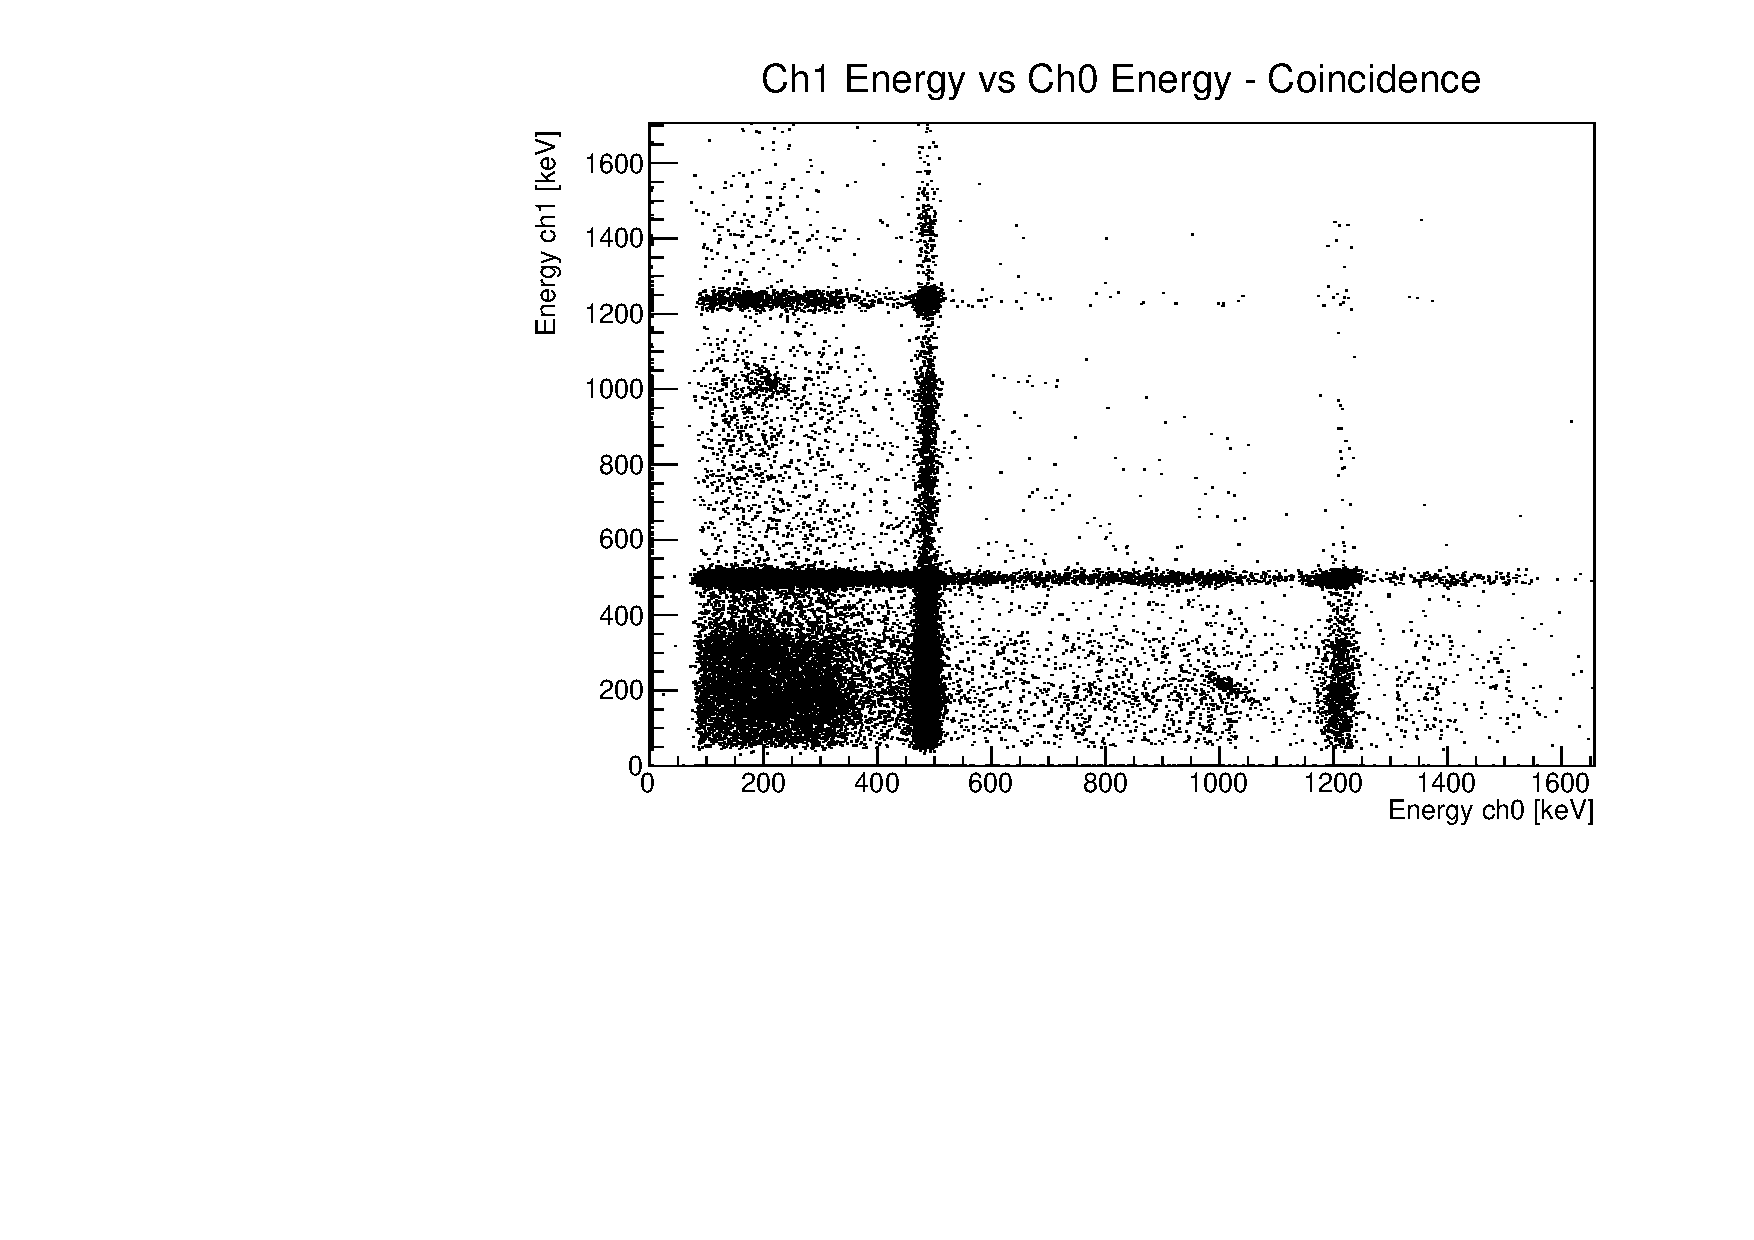
\includegraphics[width=0.9\textwidth]{Images/analysis/timing/Na_e1_vs_e2_coinc.pdf}  \label{fig:Na_ee_coinc} }
	\end{minipage}
	\caption{Histograms showing the correlation between the energy spectra of channel 0 and channel 1, without and with the imposition of timing coincidence, for the $^{22}$Na source}
    \label{fig:T_effect_Na}
	\end{figure}
 \begin{figure}[H]
	\begin{minipage}[c]{0.5\linewidth}
	\subfloat[][No timing coincidence.]{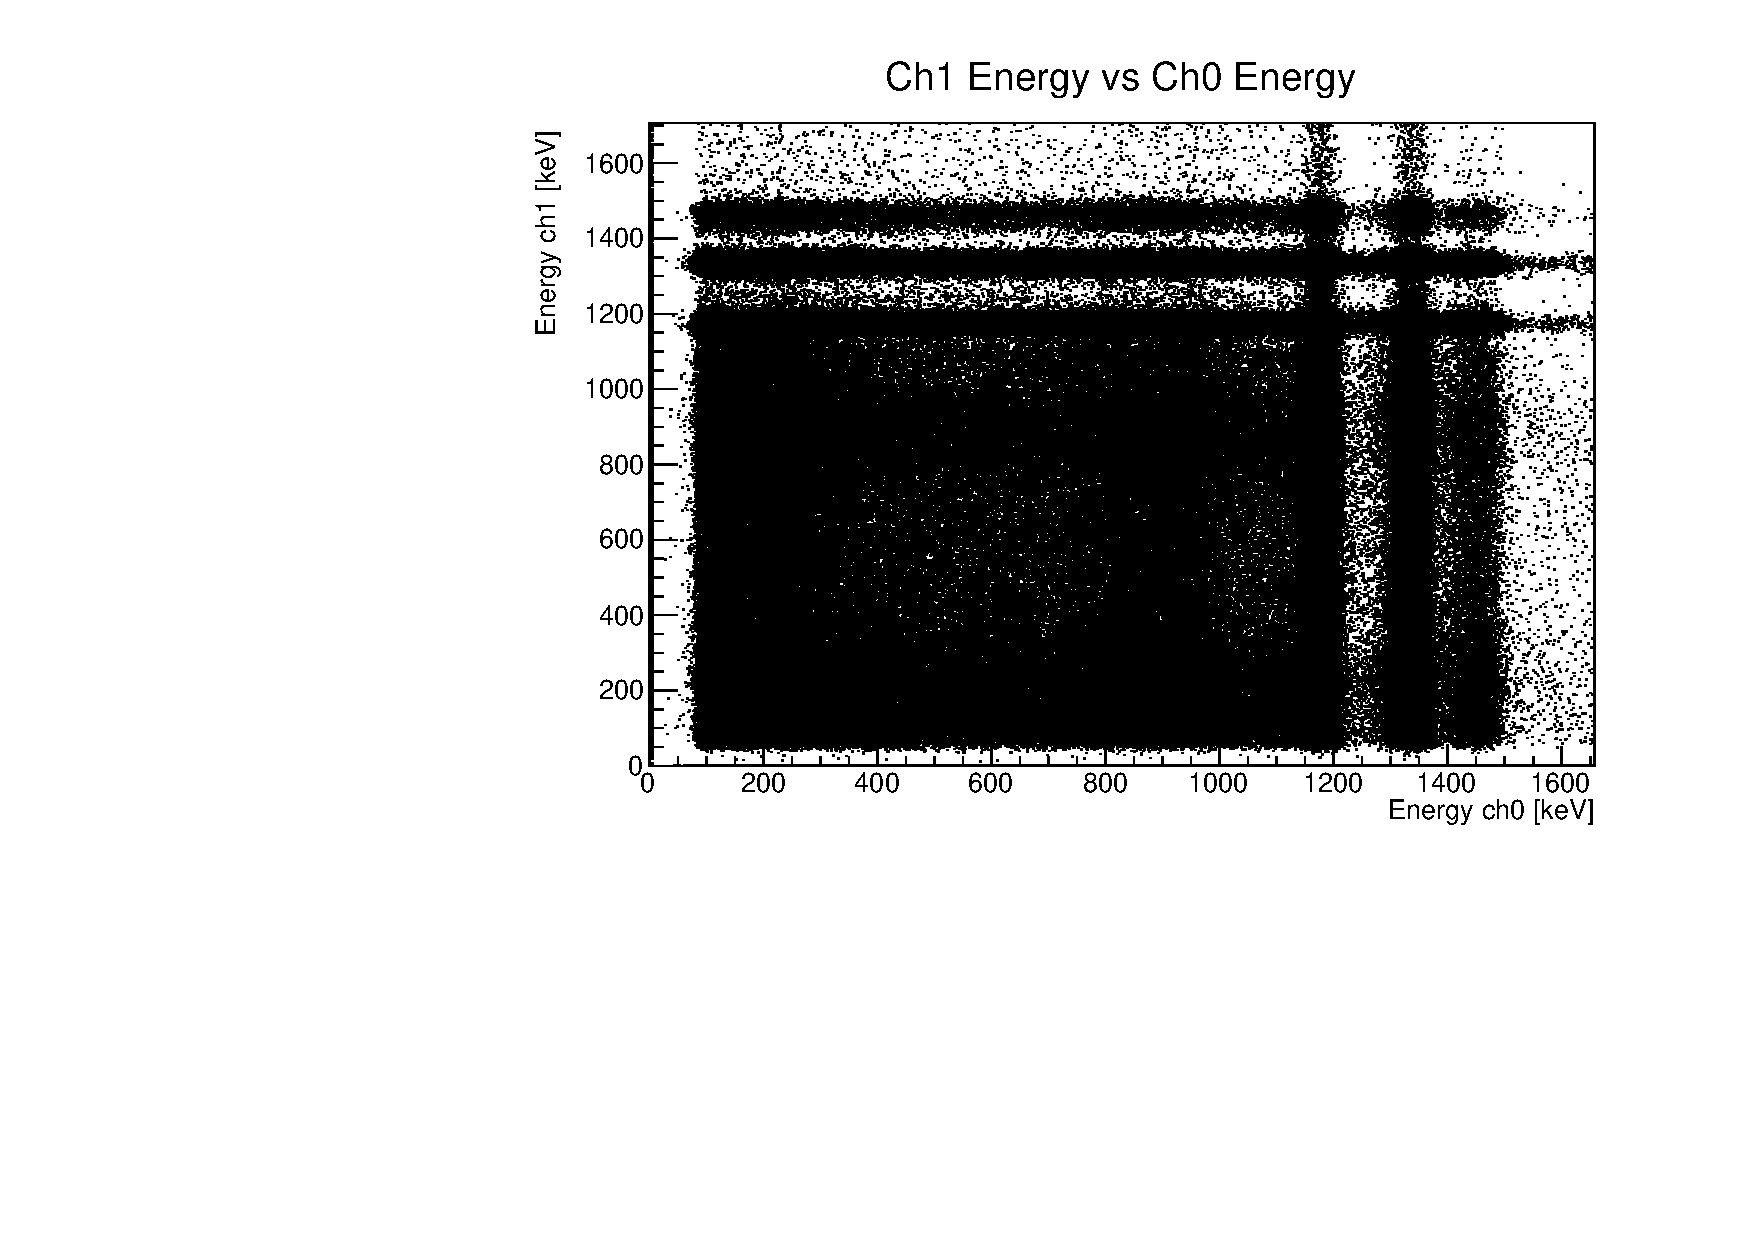
\includegraphics[width=0.9\textwidth]{Images/analysis/timing/Co_e1_vs_e2.pdf} \label{fig:Co_ee} }
	\end{minipage}
	\begin{minipage}[]{0.5\linewidth}
	\centering
	\subfloat[][Timing coincidence.]{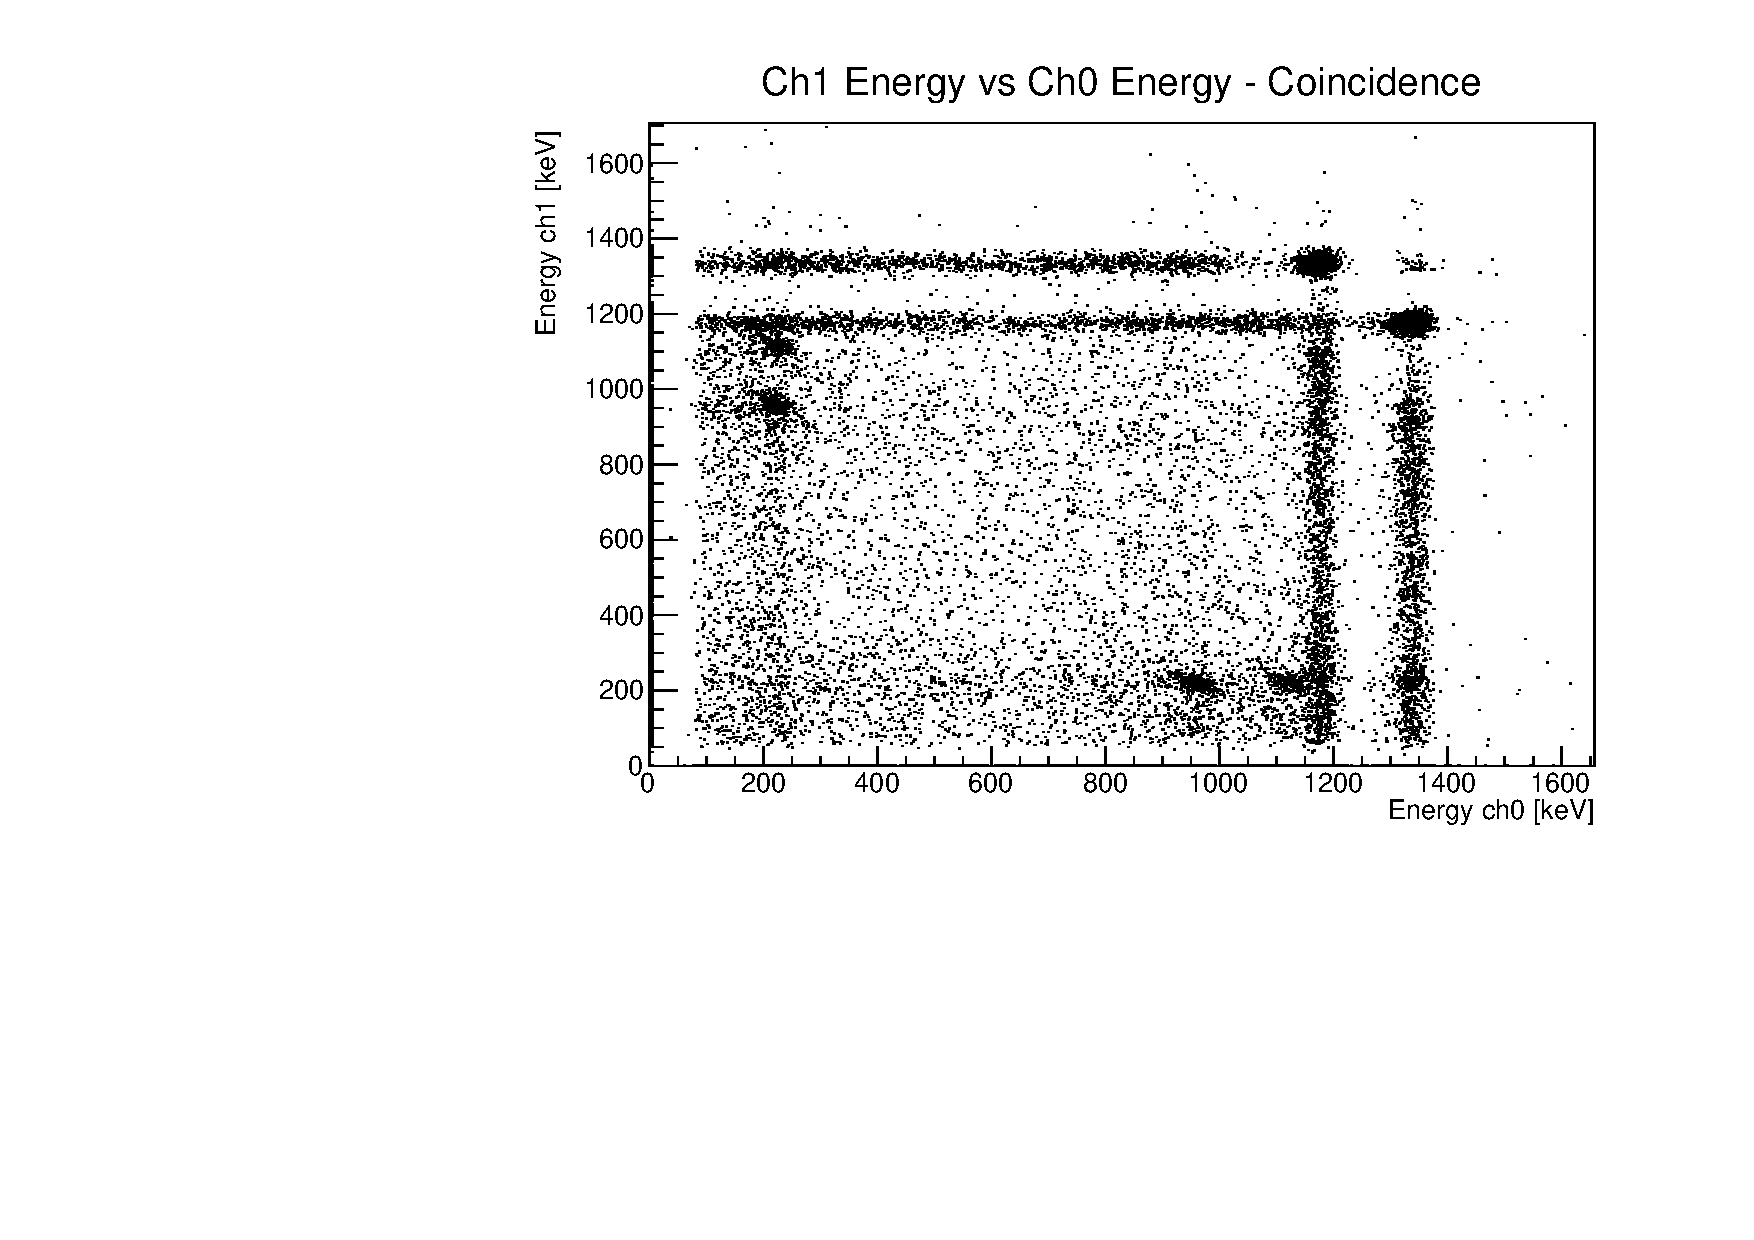
\includegraphics[width=0.9\textwidth]{Images/analysis/timing/Co_e1_vs_e2_coinc.pdf}  \label{fig:Co_ee_coinc} }
	\end{minipage}
	\caption{Histograms showing the correlation between the energy spectra of channel 0 and channel 1, without and with the imposition of timing coincidence, for the $^{60}$Co source}
    \label{fig:T_effect_Co}
	\end{figure}



\label{sec:timing}

\section{Efficiency}
\label{sec:efficiency}

Lastly, we are interested in estimating the efficiency of the detectors.
The efficiency is the number of events detected over the number of photons emitted by the source. This parameter is extremely important for the correct characterization of the detectors, and in the following subsections are listed different methods used to get this estimation.

\subsection{First Estimate}
\label{sub:rough}

\begin{comment}
\begin{figure}[H]
    \centering
    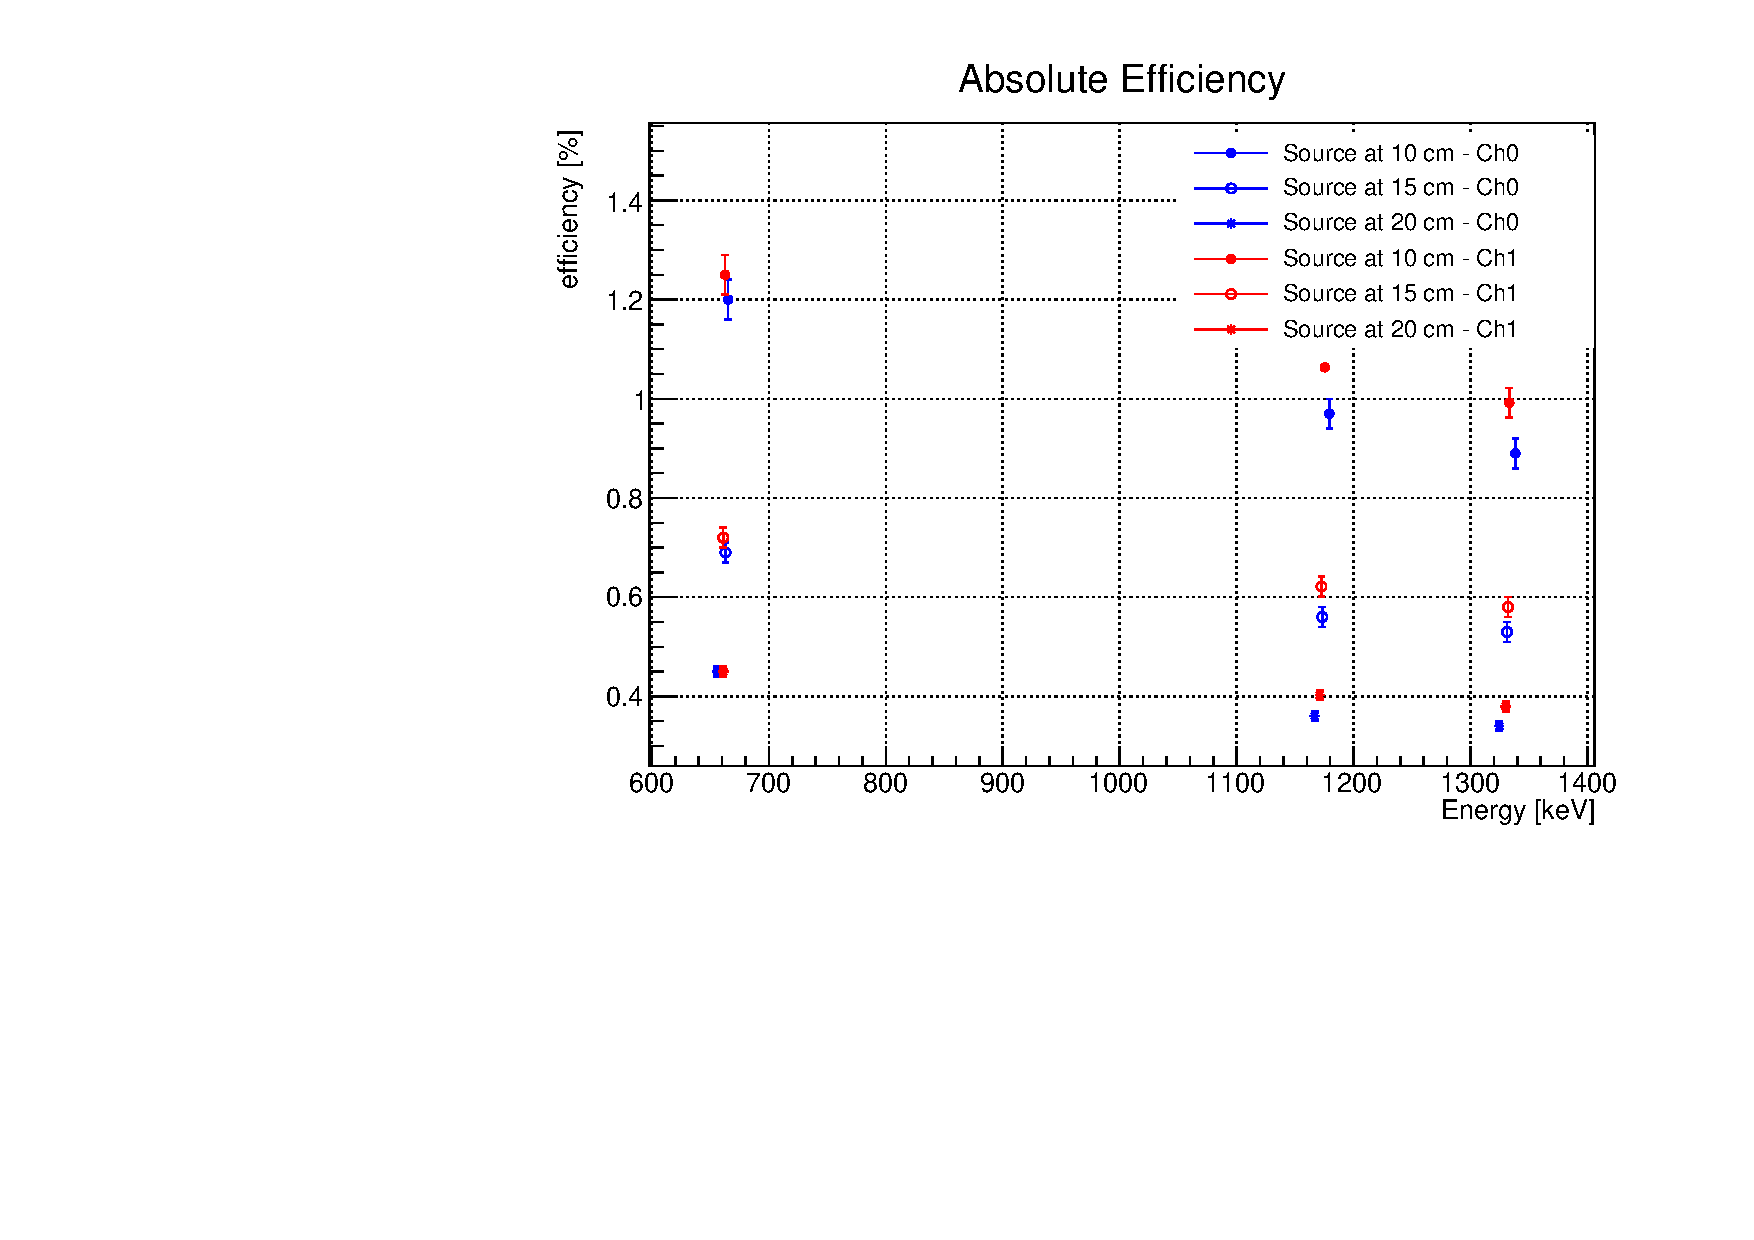
\includegraphics[scale=0.5]{Images/analysis/efficiency/eff_rough.pdf}
    \caption{First rough estimate of the absolute efficiency of the detectors, with detector 0 in blue and detector 1 in red, for each distance.}
    \label{fig:eff_rough}
\end{figure}
\end{comment}

\begin{figure}[H]
	\begin{minipage}[c]{0.35\linewidth}
    \centering
	\subfloat[][Sources at 10 cm.]{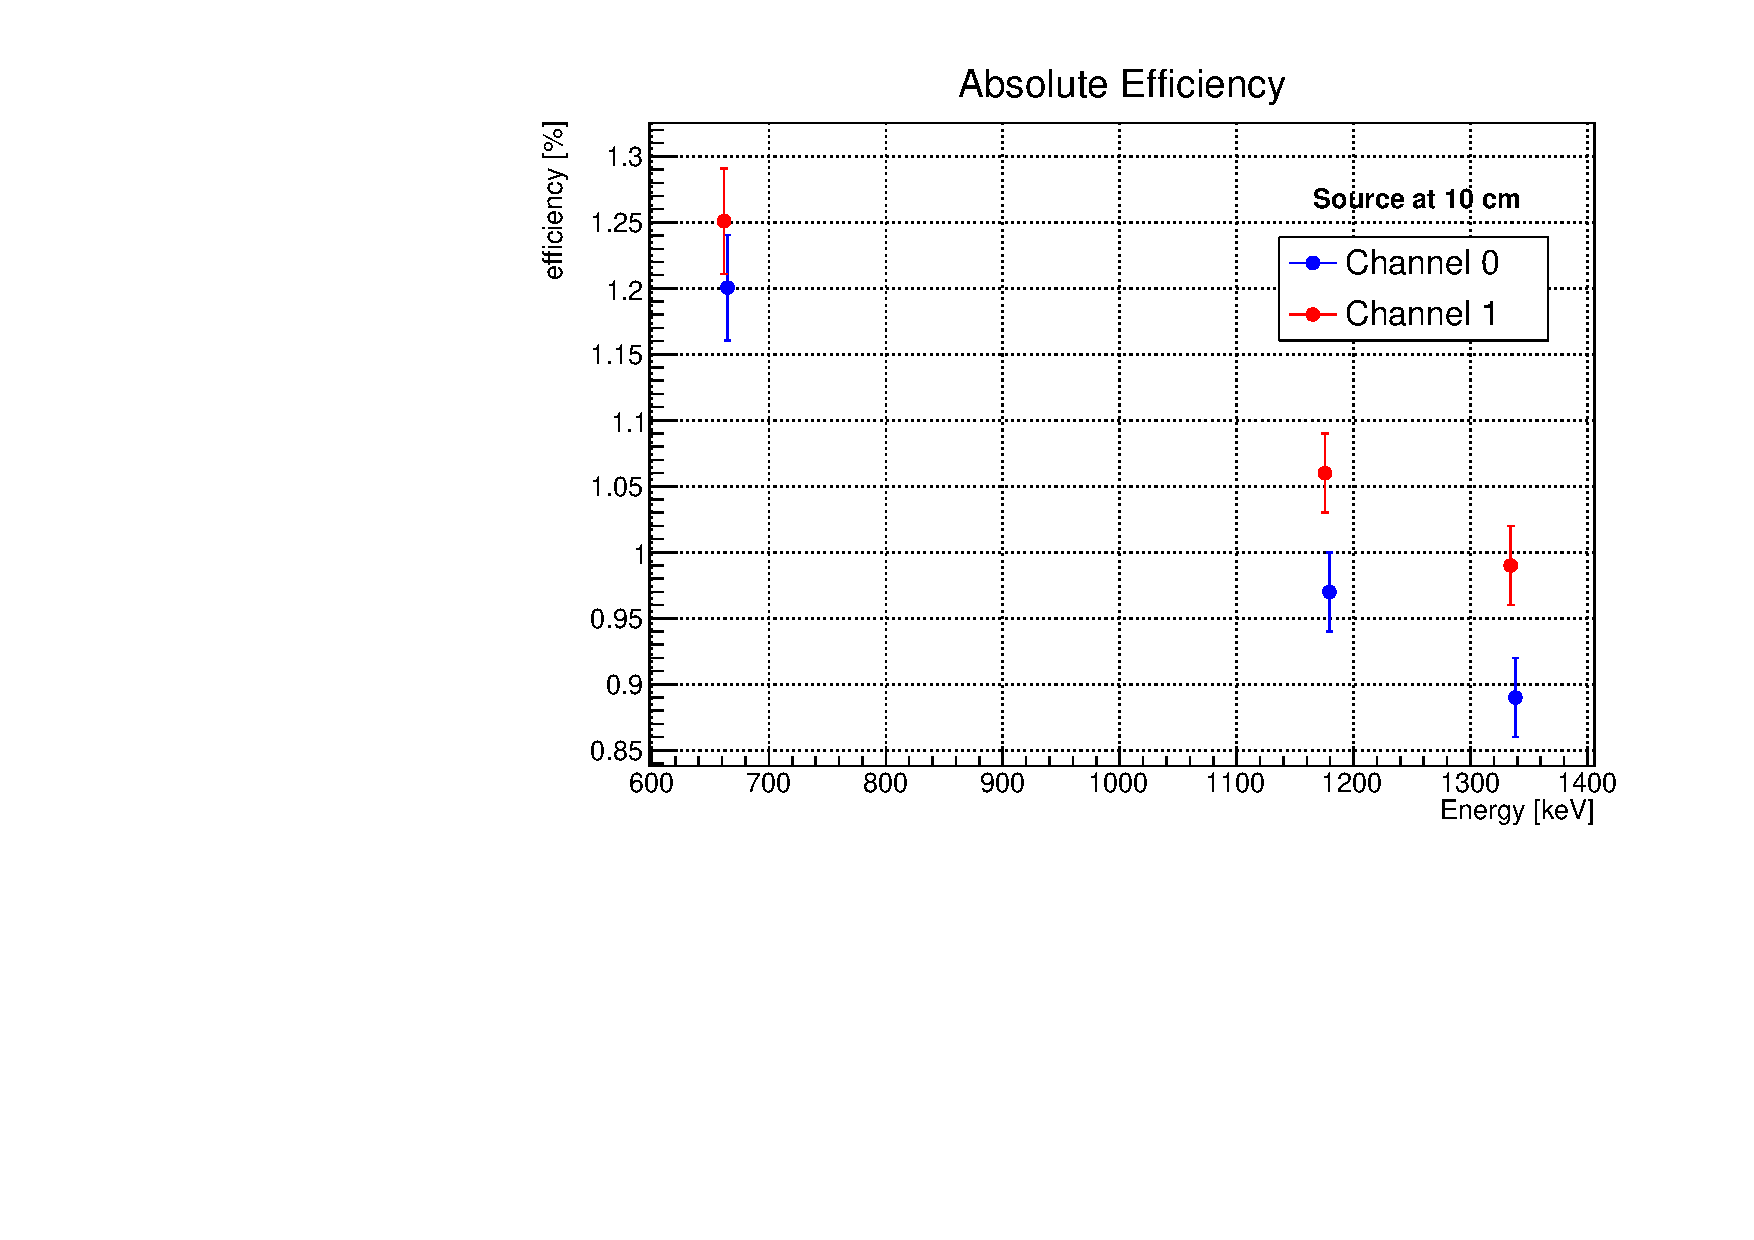
\includegraphics[width=0.95\textwidth]{Images/analysis/efficiency/eff_rough_10.pdf} \label{fig:rough_10} }
	\end{minipage}
	\begin{minipage}[]{0.35\linewidth}
	\centering
	\subfloat[][Sources at 15 cm.]{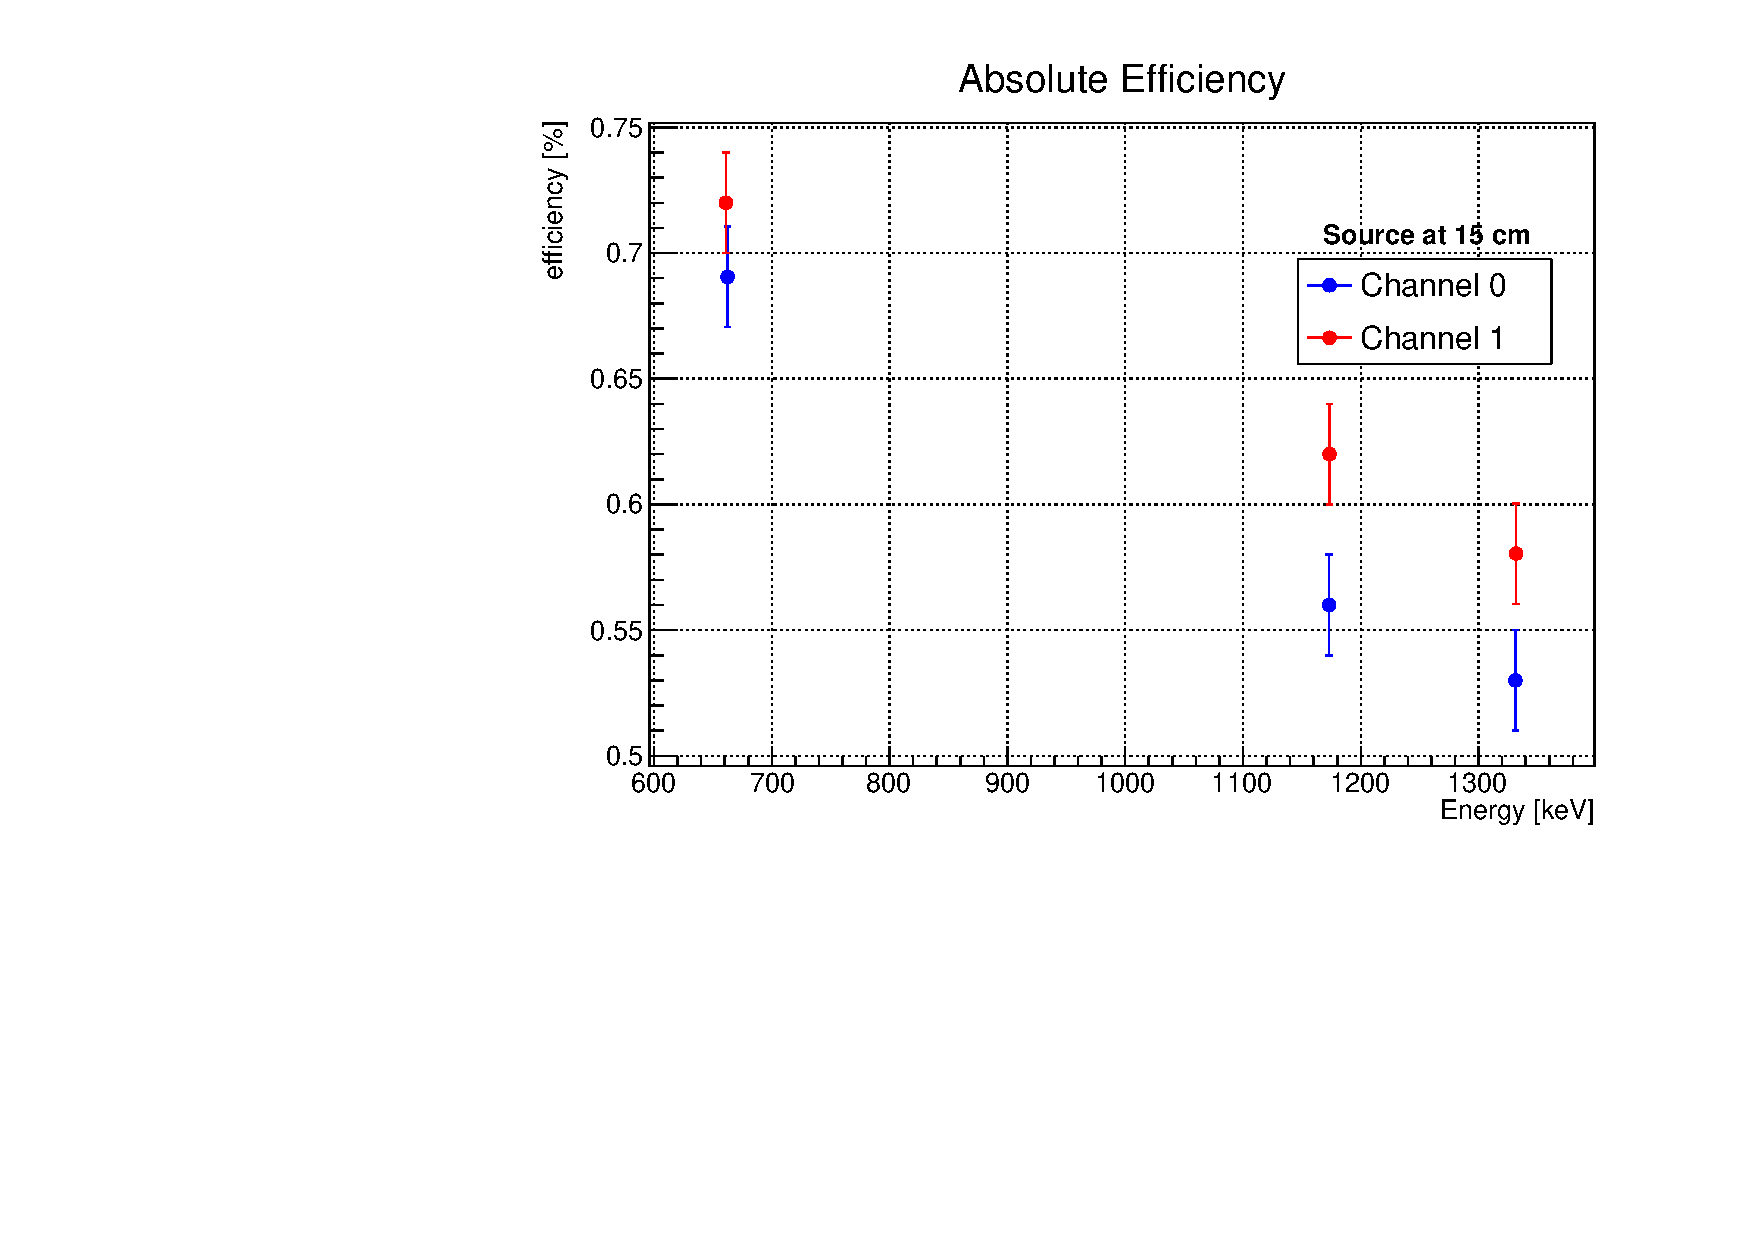
\includegraphics[width=0.95\textwidth]{Images/analysis/efficiency/eff_rough_15.pdf}  \label{fig:rough_15} }
	\end{minipage}
    \begin{minipage}[c]{0.35\linewidth}
    \centering
	\subfloat[][Source at 20 cm]{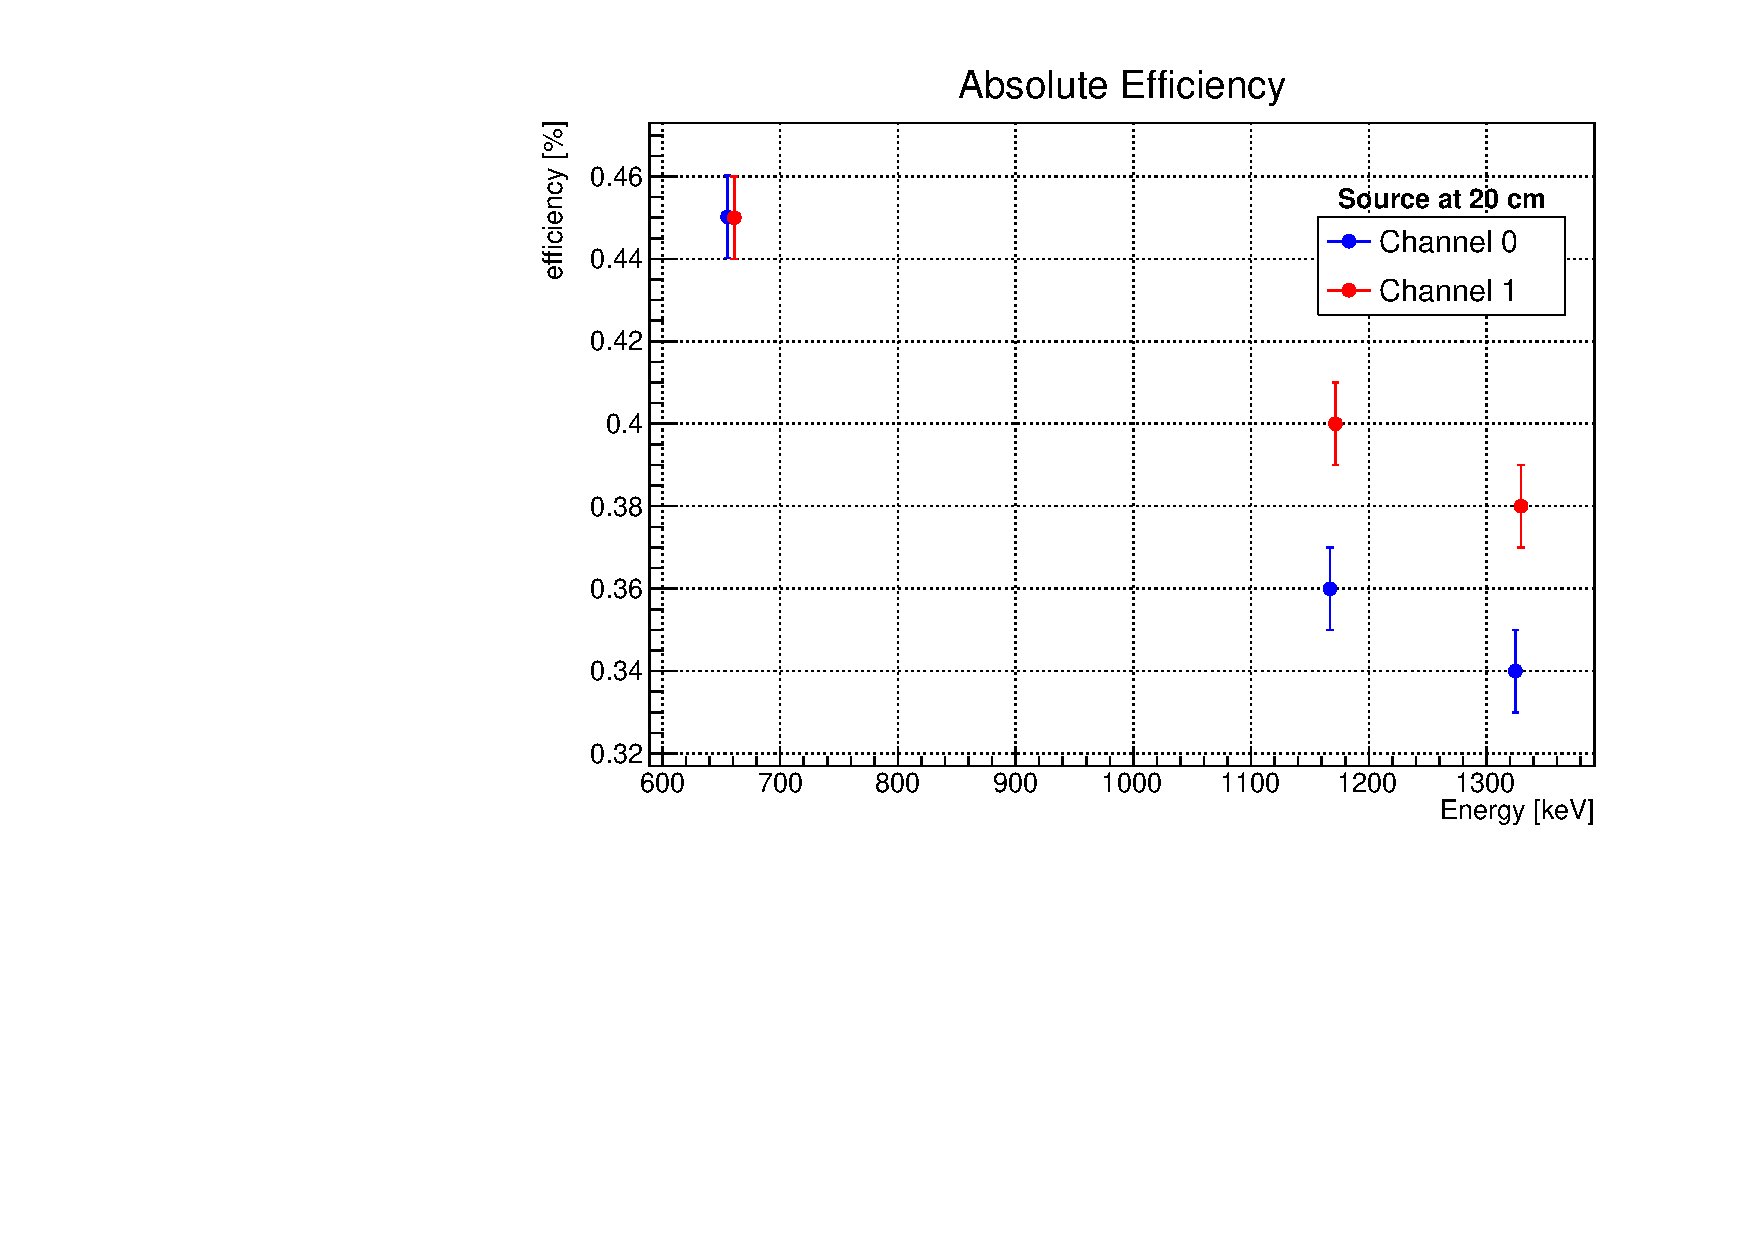
\includegraphics[width=0.95\textwidth]{Images/analysis/efficiency/eff_rough_20.pdf} \label{fig:rough_20} }
	\end{minipage}
	\caption{First rough estimate of the absolute efficiency of the detectors, with detector 0 in blue and detector 1 in red, for each distance.}
    \label{fig:eff_rough}
	\end{figure}
 
To make a first rough estimate of the efficiency, we take the peaks of $^{137}$Cs and $^{60}$Co, and compute the area subtended by the gaussian without the background, which corresponds to the number of events detected at each energy. For this first estimation, we also considere the events in the peak of 2505 keV for $^{60}$Co. This peak, as said before, corresponds to the detection of the two gammas of 1172 keV and 1332 keV from the same detector, that collects them as one event. Since the presence of this peak means that a gamma of 1172 keV, as well as a gamma of 1332 keV, are detected, we estimate the area of this peak and we add its value to both the areas of the peaks of 1172 keV and 1332 keV, to obtain the total number of events at said energy (eq. \ref{eq:events}).

\begin{equation} \label{eq:events}
    \\ N_{1173}= Area_{1173}^{peak}+Area_{2505}^{peak} \\
    N_{1332}= Area_{1332}^{peak}+Area_{2505}^{peak}
\end{equation}

To get the total number of photons actually produced by the sources, we use the values of the activity of the sources and the collection time. Once we have the number of detected events and source events, we can get the efficiency as their ratio. The trend of the efficiency at different distances from the sources is shown in fig. \ref{fig:eff_rough} and the values in tab. \ref{table:eff_rough}.

\begin{table}[h]
    \begin{subtable}
        \centering
        \begin{tabular}{|c|c|c|c|}
        \hline
        & E [keV]  & eff [\%] &$\sigma_{eff}$ [\%]  \\
        \hline
        $^{137}$Cs at 10 cm & 662 &1.20&0.04\\
        \hline
        \multirow{2}{*}{$^{60}$Co at 10 cm}&1173 &0.97 & 0.03 \\ 
        &1332 &0.89 & 0.03 \\
        \hline
        $^{137}$Cs at 15 cm & 662 &0.69&0.02\\
        \hline
        \multirow{2}{*}{$^{60}$Co at 15 cm}&1173 &0.56 & 0.02 \\ 
        &1332 &0.53 & 0.02 \\
        \hline
        $^{137}$Cs at 20 cm & 662 &0.45&0.01\\
        \hline
        \multirow{2}{*}{$^{60}$Co at 20 cm}&1173 &0.36 & 0.01 \\
        &1332 &0.34 & 0.01 \\
        \hline
        \end{tabular}
    \end{subtable}
    \qquad
    \qquad
    \qquad
    \begin{subtable}
        \centering
        \begin{tabular}{|c|c|c|c|}
        \hline
        & E [keV]  & eff [\%] &$\sigma_{eff}$ [\%]  \\
        \hline
        $^{137}$Cs at 10 cm & 662 &1.25&0.04\\
        \hline
        \multirow{2}{*}{$^{60}$Co at 10 cm}&1173 &1.06 & 0.03 \\ 
        &1332 &0.99 & 0.03 \\
        \hline
        $^{137}$Cs at 15 cm & 662 &0.72&0.02\\
        \hline
        \multirow{2}{*}{$^{60}$Co at 15 cm}&1173 &0.62 & 0.02 \\ 
        &1332 &0.58 & 0.02 \\
        \hline
        $^{137}$Cs at 20 cm & 662 &0.45&0.01\\
        \hline
        \multirow{2}{*}{$^{60}$Co at 20 cm}&1173 &0.40 & 0.01 \\
        &1332 &0.38 & 0.01 \\
        \hline
        \end{tabular}
     \end{subtable}
     \caption{Values of efficiency for the $^{60}$Co and $^{22}$Na source at different distances, for detector 0 and 1, respectively.}
     \label{table:eff_rough}
\end{table}



\subsection{With Summing Up}
\label{sub:nocoinc}

The efficiency estimated in the previous subsection is actually an approximation, as it does not consider the summing up effect. In fact, if we look for example at the full spectrum of $^{60}$Co (fig. \ref{fig:co}), we can observe that with the previous method we only took into account the peaks at 1173, 1332 and 2505 keV, but neglect the Compton continuum that is present for each peak. This corresponds to a gamma that is detected by the detector but escapes, leaving only part of its energy in the crystal. Nevertheless, this means that also the Compton continuum corresponds to a gamma detection, so this area should also be taken into account in the efficiency computation. 

\begin{figure}[H]
    \centering
    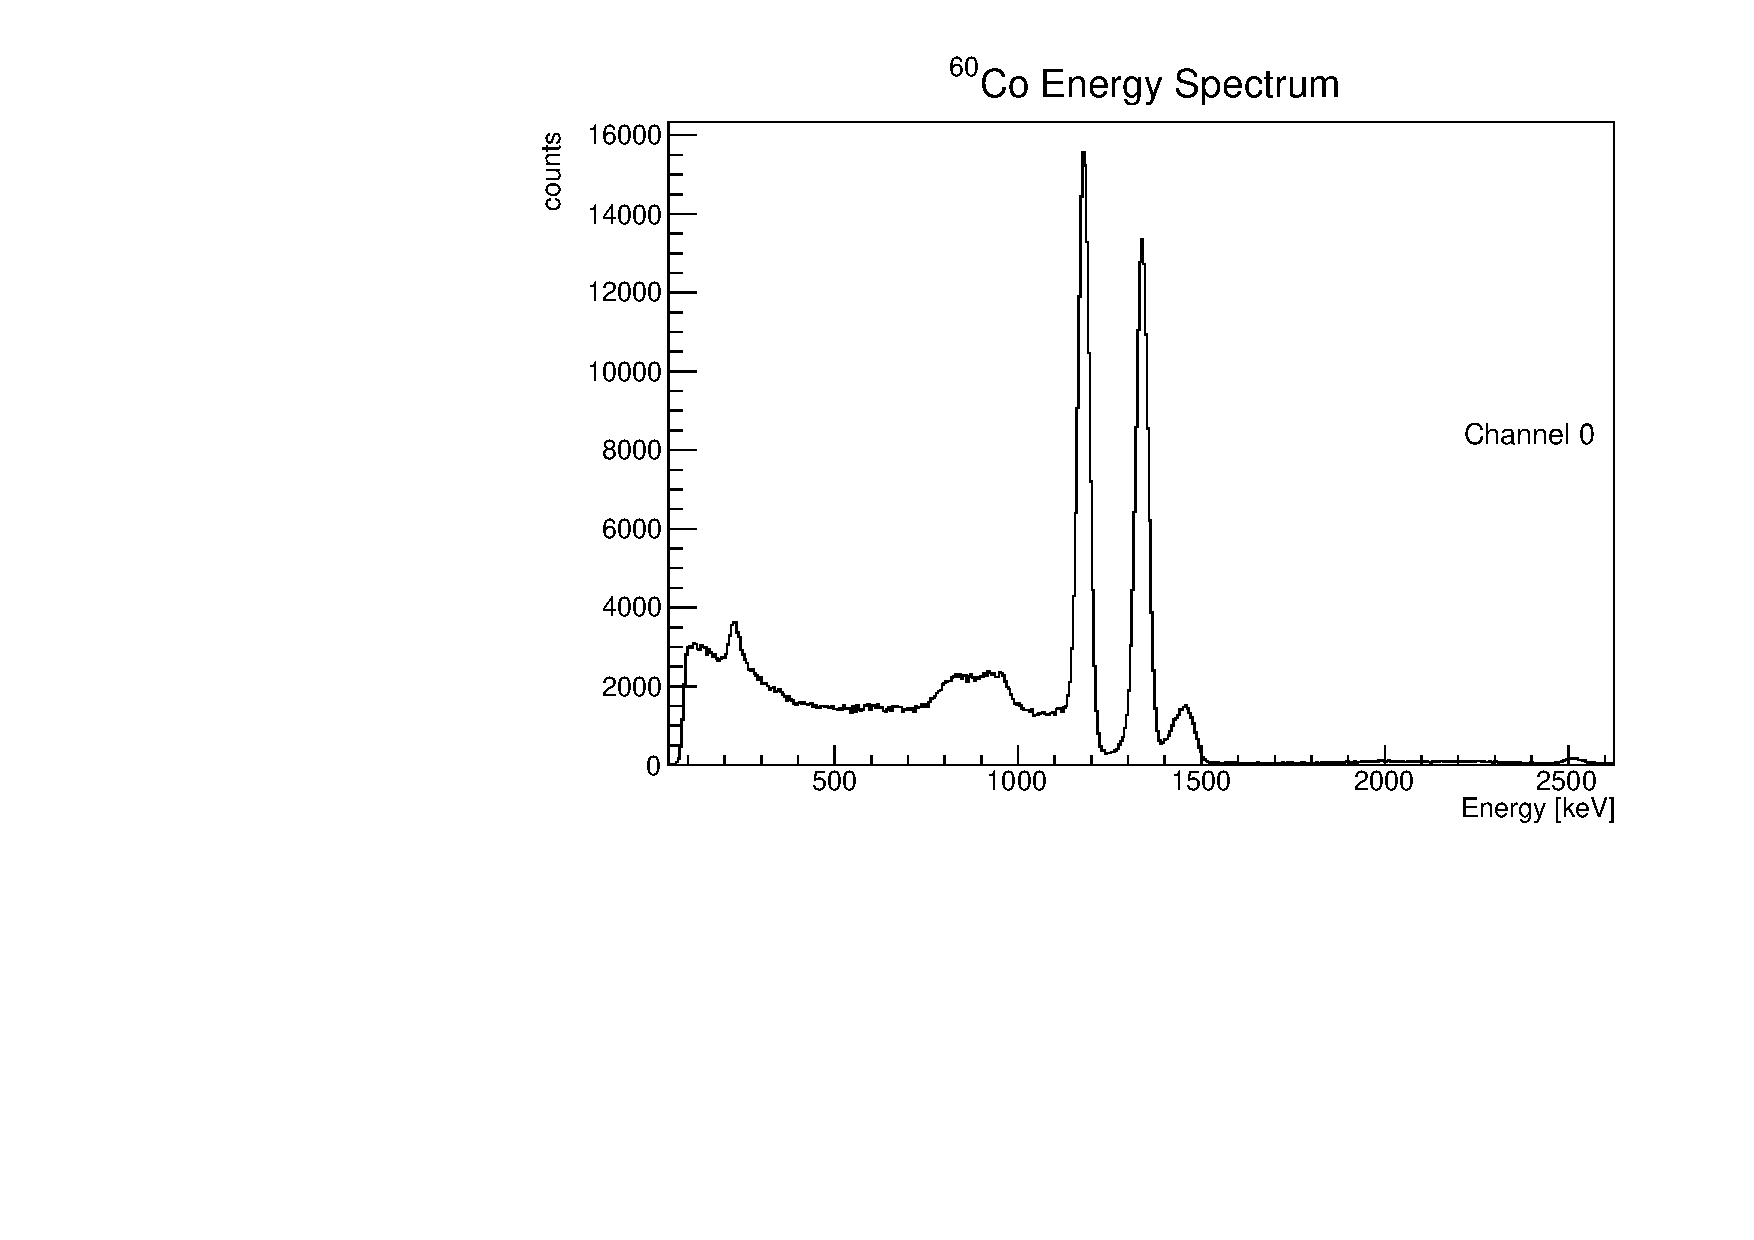
\includegraphics[scale=0.5]{Images/analysis/efficiency/Co.pdf}
    \caption{Energy spectrum of $^{60}$Co at 10 cm, for detector 0.}
    \label{fig:co}
\end{figure}

In order consider the summing up effect, the total efficiency is obtained using eq. \ref{eq:eta}

\begin{equation} \label{eq:eta}
    \eta=\eta_{peak} \, (1-\eta_{tot})
\end{equation}

where $\eta_{peak}$ is the efficiency obtained by considering the events in the peak and $\eta_{tot}$ is the efficiency obtained considering the total event of the spectrum as the number of event detected. \\

In this section, the data from $^{22}$Na source is also used. The results for all sources are shown in tab. \ref{tab:eff_nocoinc}. \\
The trend of the absolute efficiencies, shown in fig. \ref{fig:eff_nocoinc}, resembles the one obtained with the rough estimate in fig. \ref{fig:eff_rough}. We then estimate their compatibility for $^{60}$Co and $^{137}$Cs, and show the results in tab. \ref{tab:eff_comp}. The two methods provide compatible results.

\begin{figure}[H]
    \centering
    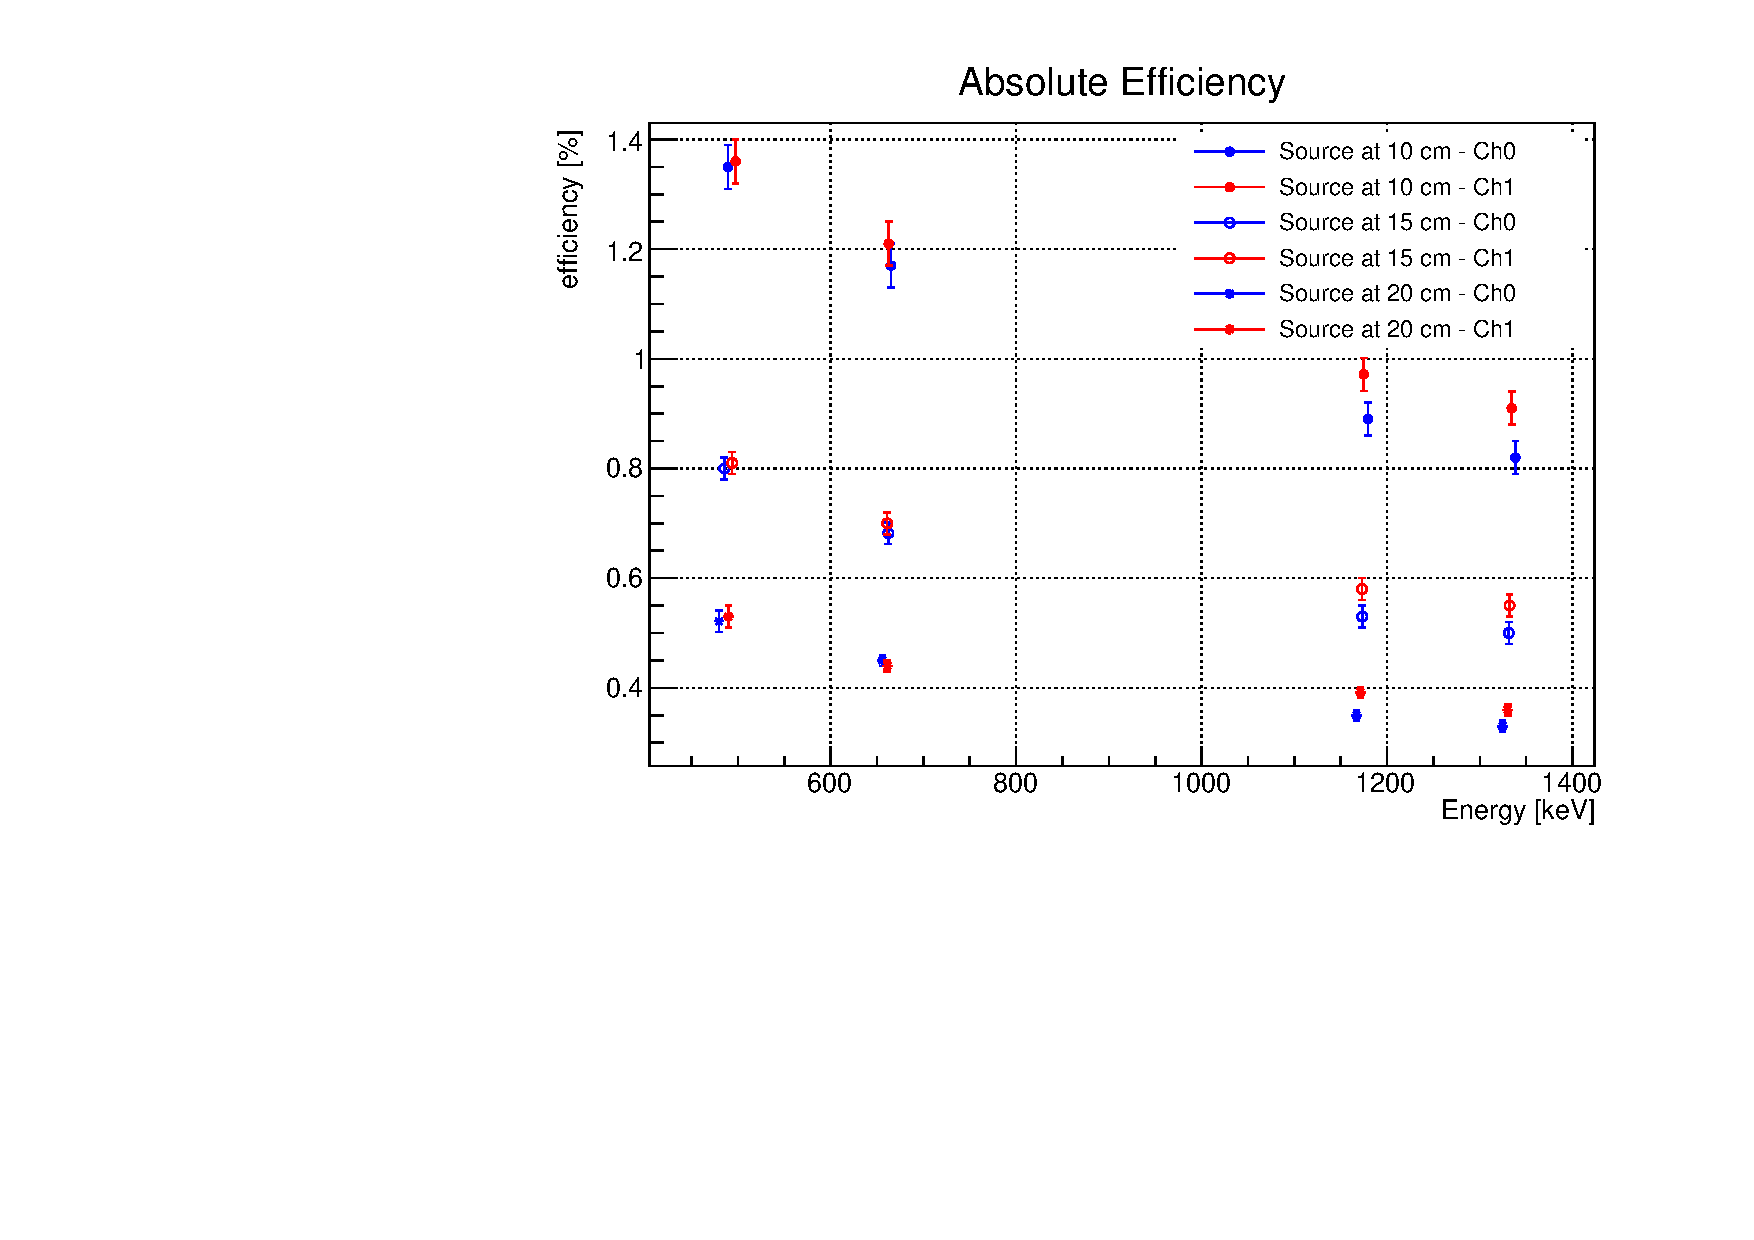
\includegraphics[scale=0.5]{Images/analysis/efficiency/Eff_nocoinc.pdf}
    \caption{Efficiency of the detectors, without using coincidences and considering summing up as in \ref{eq:eta}, with detector 0 in blue and detector 1 in red, for all the distances.}
    \label{fig:eff_nocoinc}
\end{figure}

\begin{figure}[H]
	\begin{minipage}[c]{0.35\linewidth}
    \centering
	\subfloat[][Sources at 10 cm.]{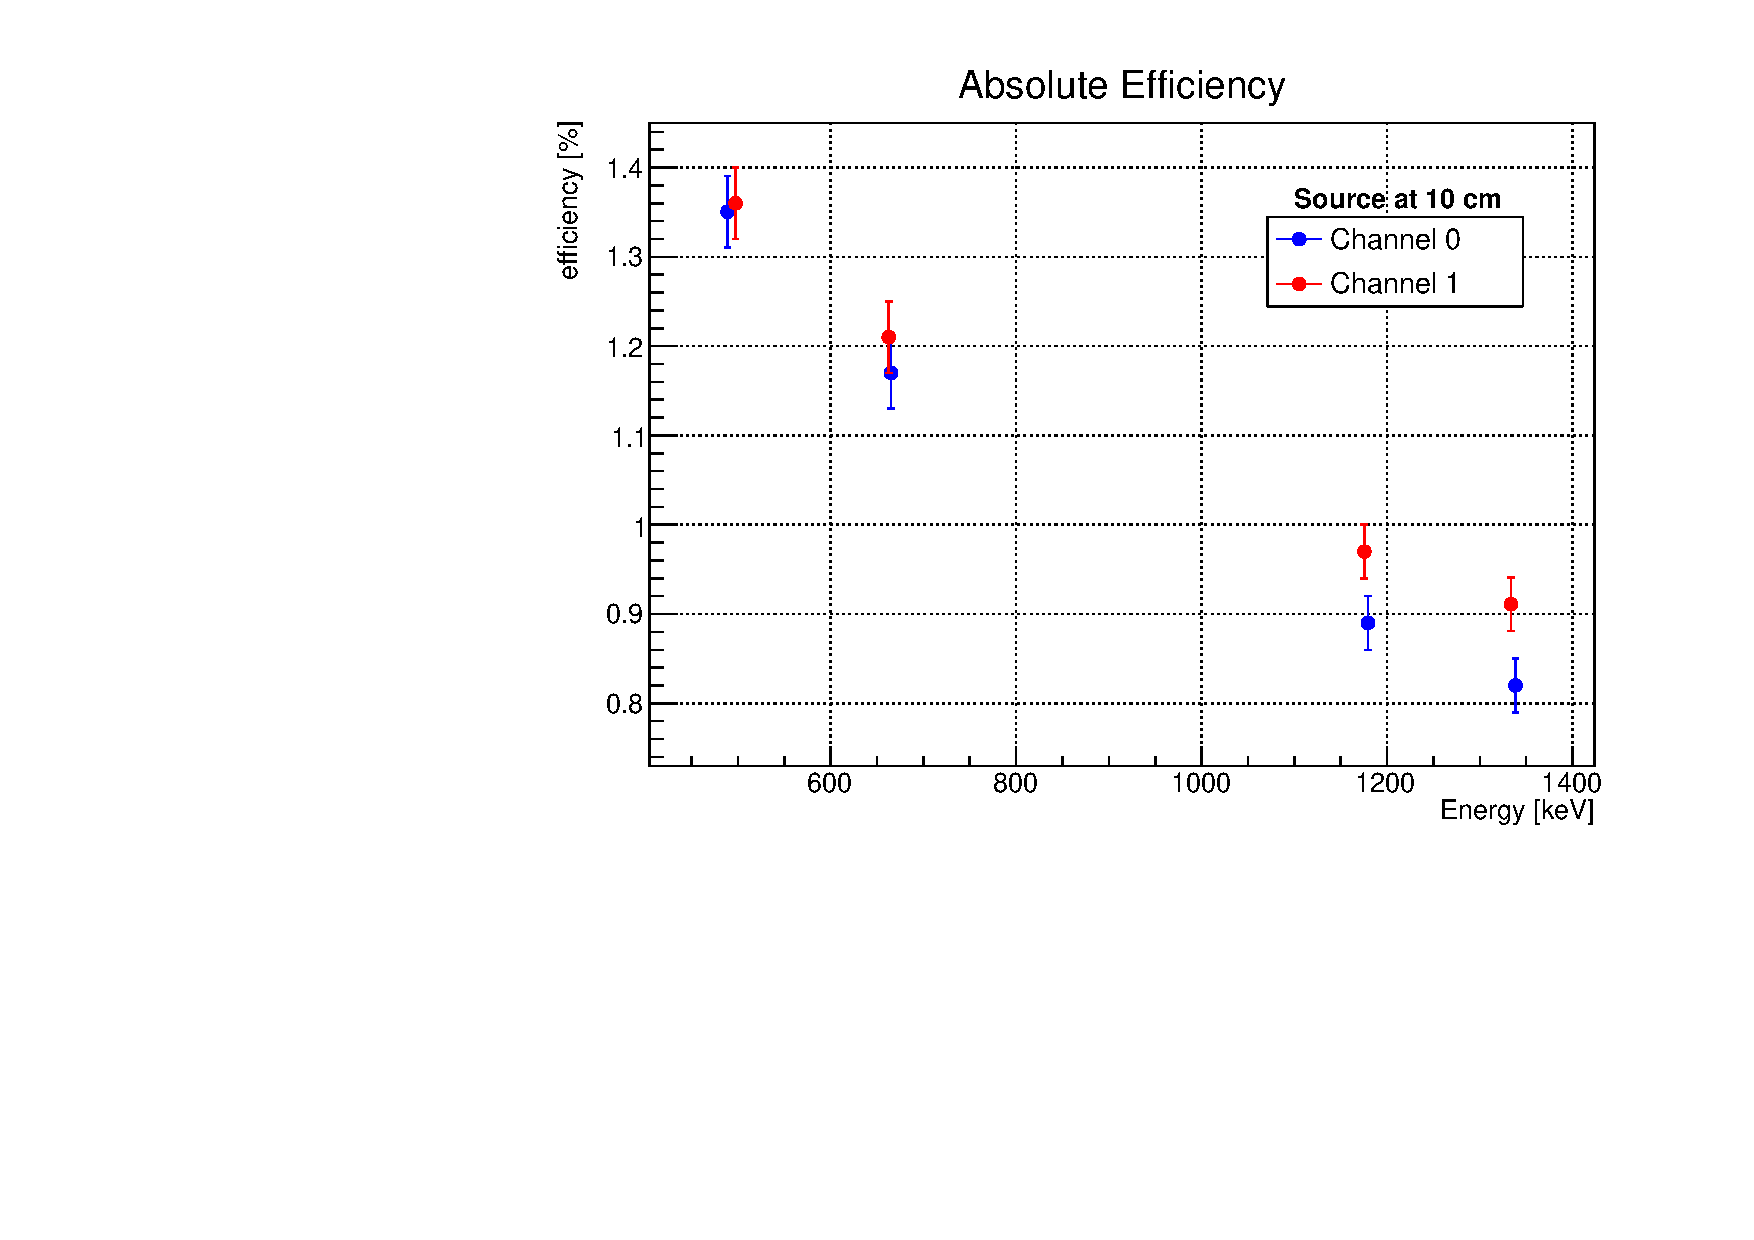
\includegraphics[width=0.95\textwidth]{Images/analysis/efficiency/eff_nocoinc_10.pdf} \label{fig:nocoinc_10} }
	\end{minipage}
	\begin{minipage}[]{0.35\linewidth}
	\centering
	\subfloat[][Sources at 15 cm.]{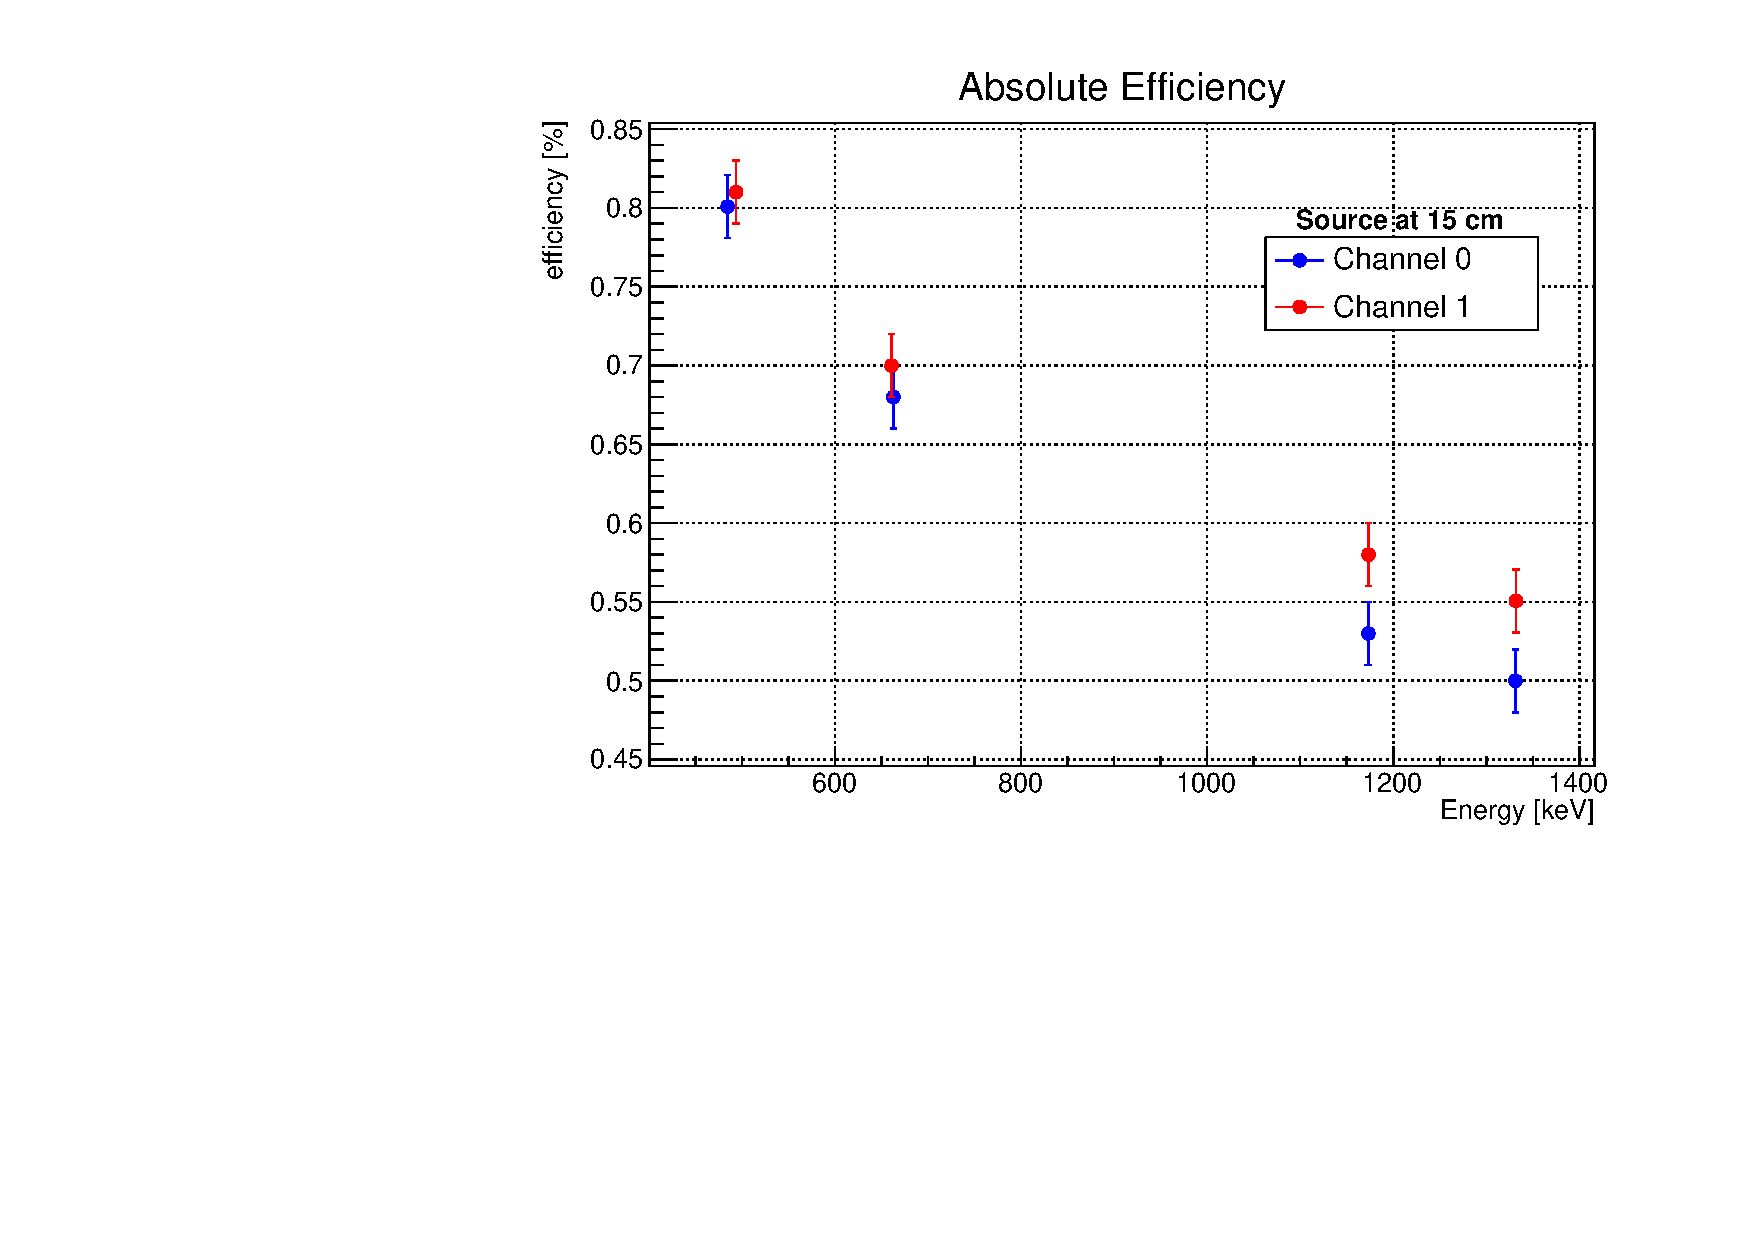
\includegraphics[width=0.95\textwidth]{Images/analysis/efficiency/eff_nocoinc_15.pdf}  \label{fig:nocoinc_15} }
	\end{minipage}
    \begin{minipage}[c]{0.35\linewidth}
    \centering
	\subfloat[][Source at 20 cm]{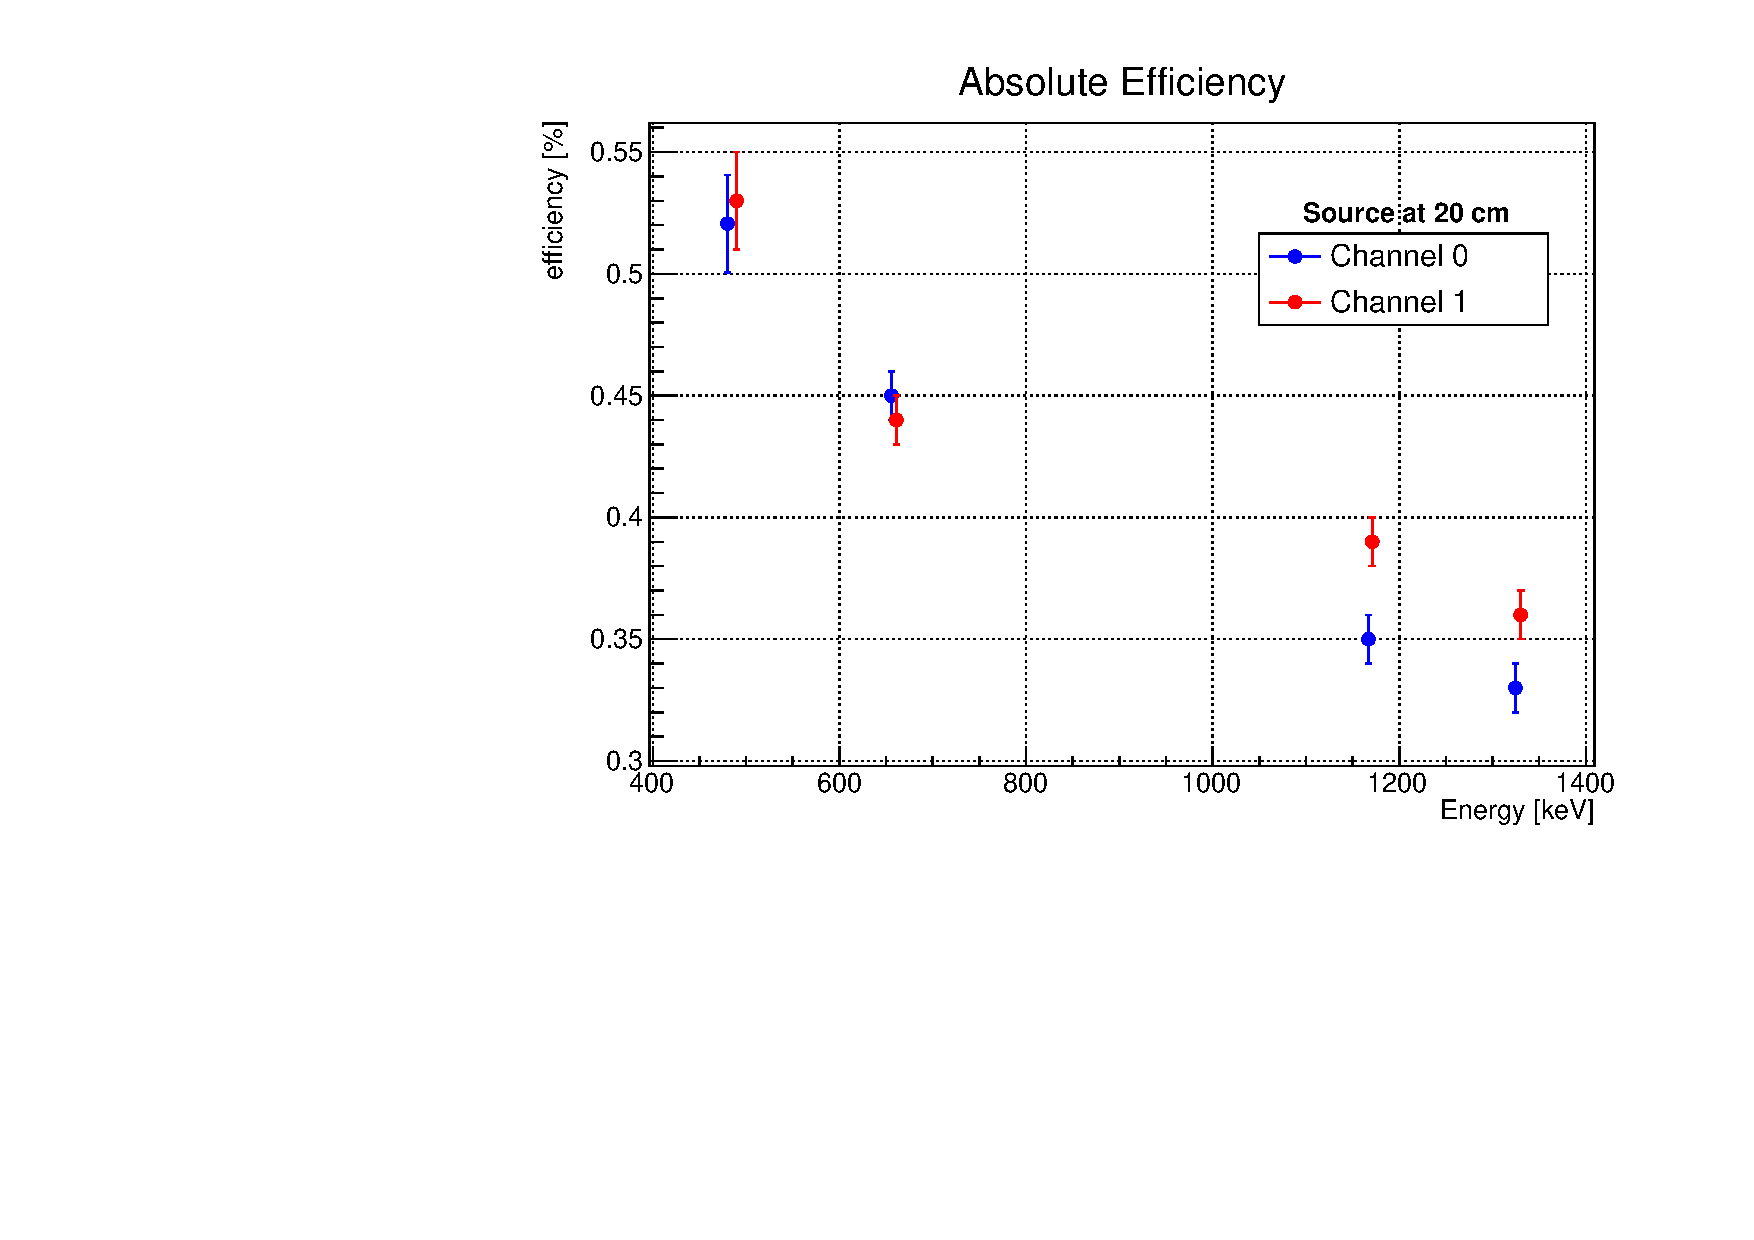
\includegraphics[width=0.95\textwidth]{Images/analysis/efficiency/eff_nocoinc_20.pdf}} \label{fig:nocoinc_20} 
	\end{minipage}
	\caption{Efficiency of the detectors, without using coincidences and considering summing up as in \ref{eq:eta}, with detector 0 in blue and detector 1 in red, at each different distances for each plot.}
    \label{fig:eff_nocoinc3}
	\end{figure}



\begin{table}[h]
    \begin{subtable}
        \centering
        \begin{tabular}{|c|c|c|c|}
        \hline
        & E [keV]  & eff [\%] &$\sigma_{eff}$ [\%]  \\
        \hline
        $^{22}$Na at 10 cm & 511 &1.35&0.04\\
        \hline
        $^{137}$Cs at 10 cm & 662 & 1.17 & 0.04\\
        \hline
        \multirow{2}{*}{$^{60}$Co at 10 cm}&1173 &0.89 & 0.03 \\ 
        &1332 &0.82 & 0.03 \\
        \hline
        $^{22}$Na at 15 cm & 511 &0.80&0.02\\
        \hline
        $^{137}$Cs at 15 cm & 662 & 0.68 & 0.02\\
        \hline
        \multirow{2}{*}{$^{60}$Co at 15 cm}&1173 &0.53 & 0.02 \\ 
        &1332 &0.50 & 0.02 \\
        \hline
        $^{22}$Na at 20 cm & 511 &0.52&0.02\\
        \hline
        $^{137}$Cs at 20 cm & 662 & 0.45 & 0.01\\
        \hline
        \multirow{2}{*}{$^{60}$Co at 20 cm}&1173 &0.35 & 0.01 \\
        &1332 &0.33 & 0.01 \\
        \hline
        \end{tabular}
    \end{subtable}
    \qquad
    \qquad
    \qquad
    \begin{subtable}
        \centering
        \begin{tabular}{|c|c|c|c|}
        \hline
        & E [keV]  & eff [\%] &$\sigma_{eff}$ [\%]  \\
        \hline
        $^{22}$Na at 10 cm & 511 &1.36&0.04\\
        \hline
        $^{137}$Cs at 10 cm & 662 & 1.21 & 0.04\\
        \hline
        \multirow{2}{*}{$^{60}$Co at 10 cm}&1173 &0.97 & 0.03 \\ 
        &1332 &0.91 & 0.03 \\
        \hline
        $^{22}$Na at 15 cm & 511 &0.81&0.02\\
        \hline
        $^{137}$Cs at 15 cm & 662 &0.70 & 0.02\\
        \hline
        \multirow{2}{*}{$^{60}$Co at 15 cm}&1173 &0.58 & 0.02 \\ 
        &1332 &0.55 & 0.02 \\
        \hline
        $^{22}$Na at 20 cm & 511 &0.53&0.02\\
        \hline
        $^{137}$Cs at 20 cm & 662 & 0.44 & 0.01\\
        \hline
        \multirow{2}{*}{$^{60}$Co at 20 cm}&1173 &0.39 & 0.01 \\
        &1332 &0.36 & 0.01 \\
        \hline
        \end{tabular}
     \end{subtable}
     \caption{Values of efficiency for all the sources at different distances, considering summing up, for detector 0 and 1 respectively.}
     \label{tab:eff_nocoinc}
\end{table}

\begin{table}[h]
    \begin{subtable}
        \centering
        \begin{tabular}{|c|c|c|c|}
        \hline
        $\lambda$& 10 cm & 15 cm & 20 cm  \\
        \hline
        662 keV & 0.7 & 0.5 & 0.4 \\
        1173 keV& 1.7 & 1.1 & 0.8 \\
        1132 keV& 1.8 & 1.1 & 0.8 \\
        \hline
        \end{tabular}
    \end{subtable}
    \qquad
    \qquad
    \qquad
    \begin{subtable}
        \centering
        \begin{tabular}{|c|c|c|c|}
        \hline
        $\lambda$ & 10 cm & 15 cm & 20 cm \\
        \hline
        662 keV & 0.8 & 0.5 & 0.4 \\
        1173 keV& 1.8 & 1.2 & 0.8 \\
        1132 keV& 1.9 & 1.2 & 0.8 \\
        \hline
        \end{tabular}
     \end{subtable}
     \caption{Compatibility between the efficiencies obtained in sec. \ref{sub:rough} and sec. \ref{sub:nocoinc}, between every value at each distance and energy, with detector 0 in the first table and detector 1 in the second.}
     \label{tab:eff_comp}
\end{table}



\subsection{With Coincidences}

In this section we want to compute the efficiency of the detectors more accurately by exploiting the coincidences between the gamma emissions in the decays of $^{22}$Na and $^{60}$Co. In sec. \ref{sec:timing} we established that two events from different channels can be considered in coincidence if their time difference is less than 16 ns. Since we want to analyze only the events in coincidence, we plot the energy spectra for each channel, imposing the condition that an event in the other channel must have a time difference smaller then 16 ns (fig.\ref{fig:coinc_spectra}). 

\begin{figure}[H]
	\begin{minipage}[c]{0.5\linewidth}
	\subfloat[][$^{60}$Co source at 10 cm.]{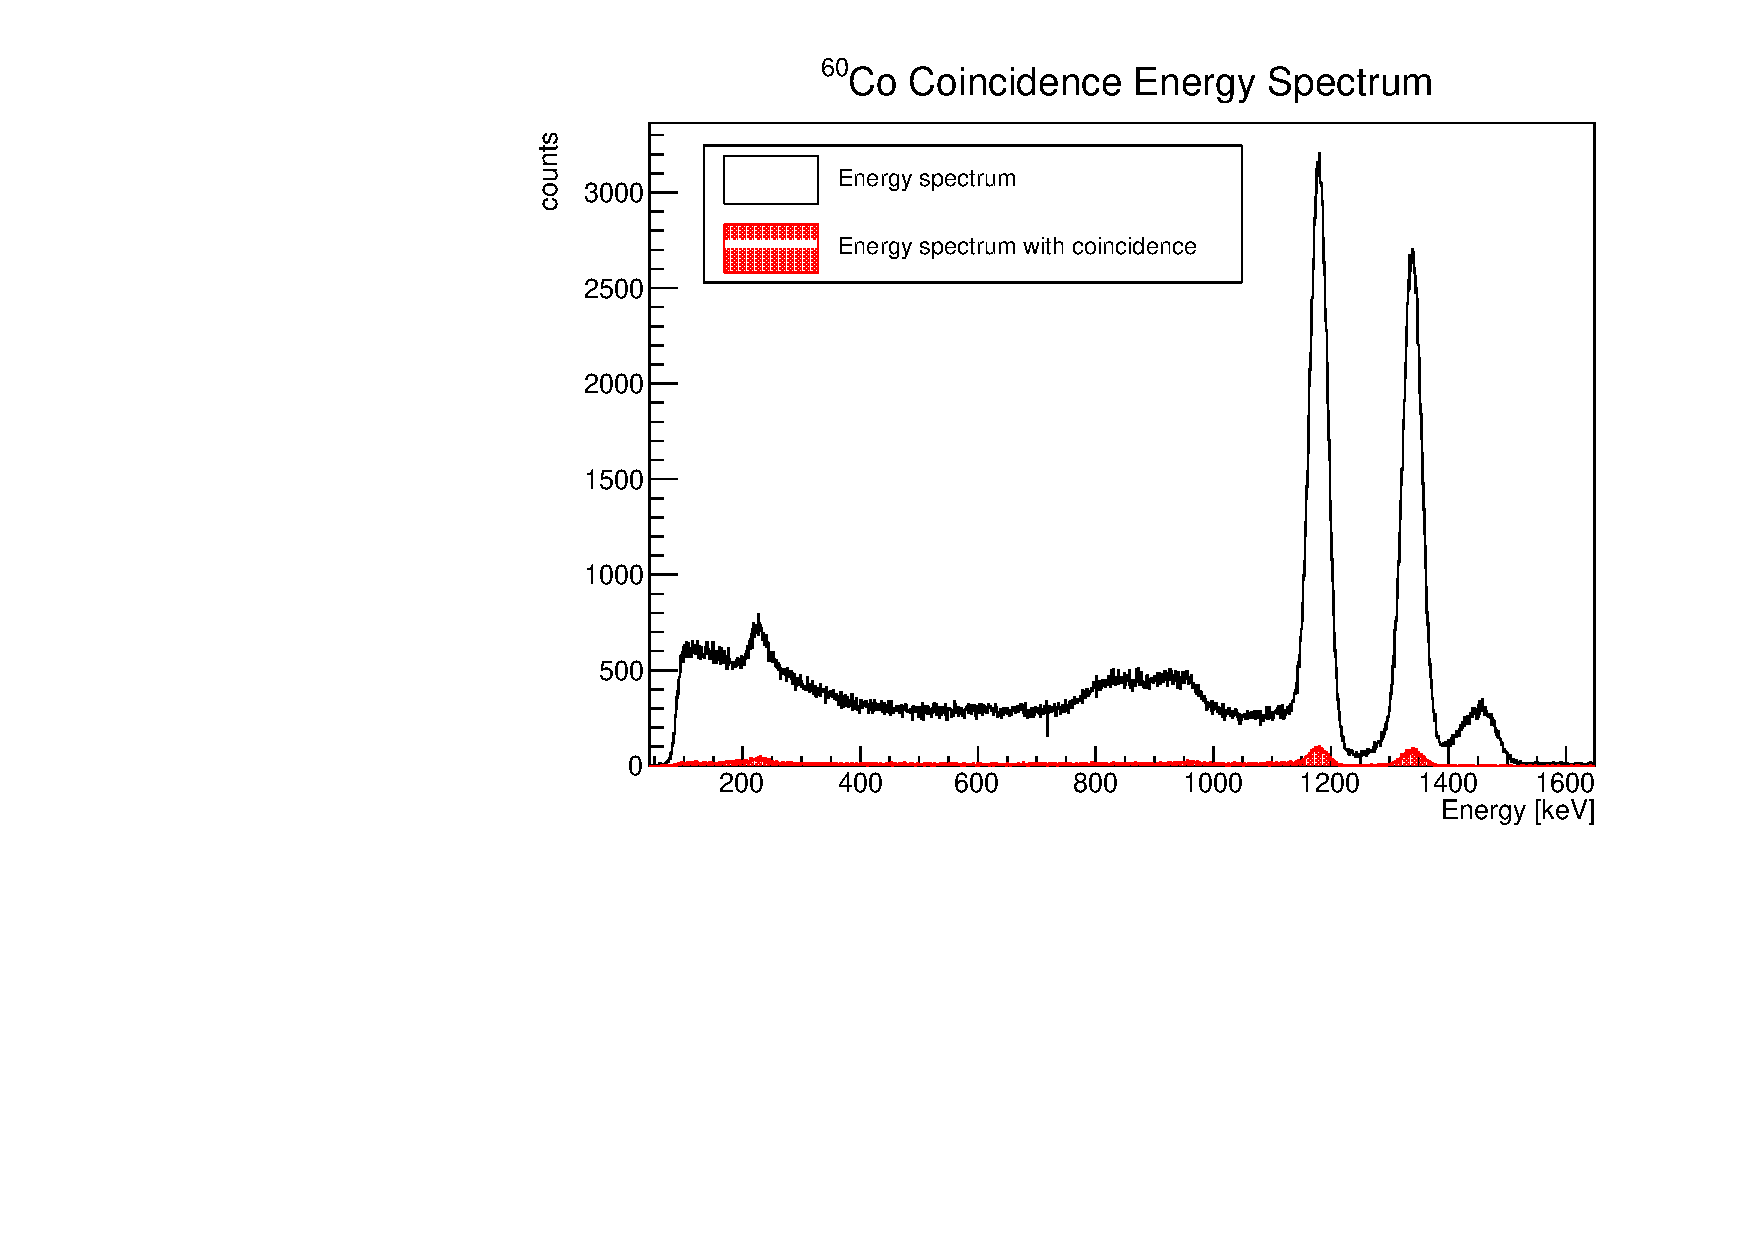
\includegraphics[width=0.9\textwidth]{Images/analysis/efficiency/Co_coinc_both.pdf} \label{fig:Co_coinc} }
	\end{minipage}
	\begin{minipage}[]{0.5\linewidth}
	\centering
	\subfloat[][$^{22}$Na source at 10 cm.]{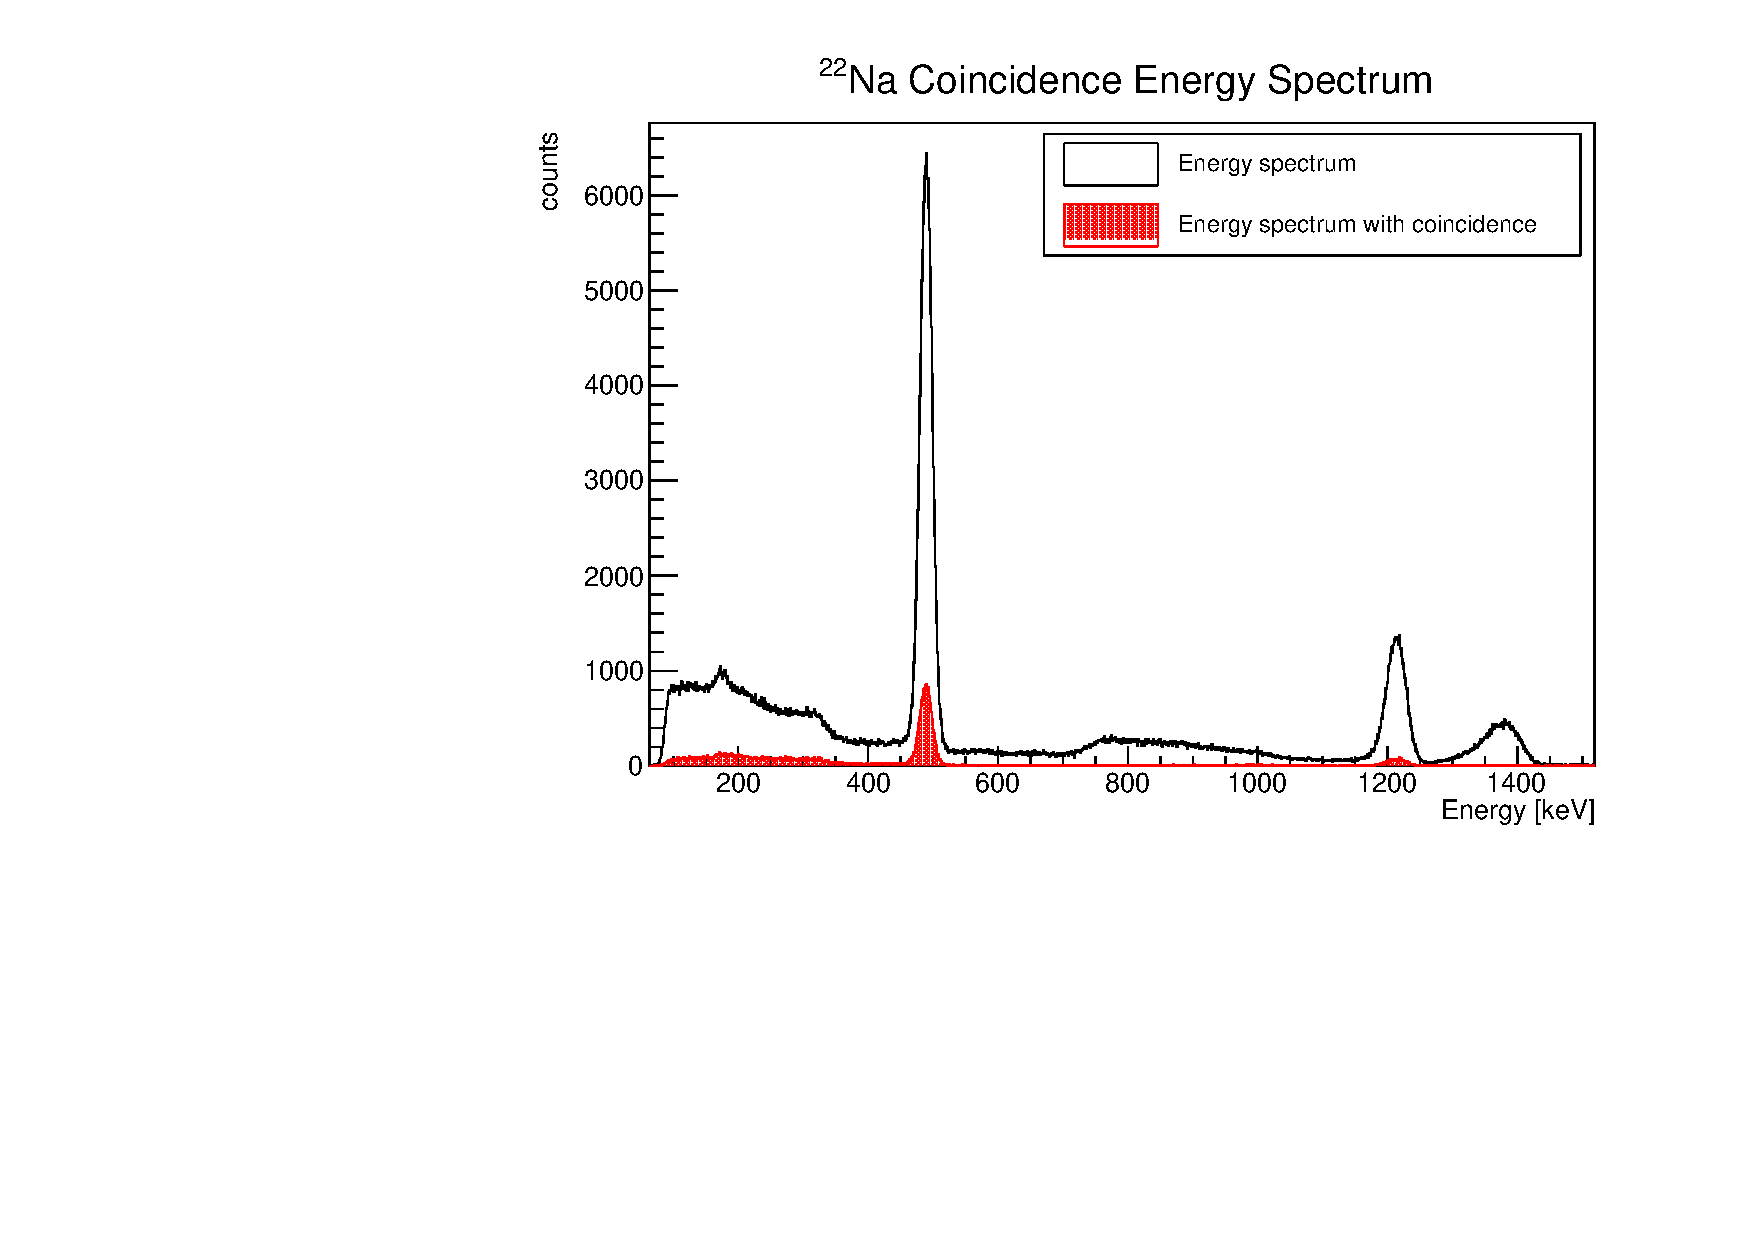
\includegraphics[width=0.9\textwidth]{Images/analysis/efficiency/Na_coinc_both.pdf}  \label{fig:Na_coinc} }
	\end{minipage}
	\caption{Comparison between the initial energy spectra of $^{60}$Co and $^{22}$Na, in black, and the energy spectra obtained imposing coincidence between the two detectors, in red, both spectra regard detector 0.}
    \label{fig:coinc_spectra}
	\end{figure}

Once we obtain these spectra, we estimate the number of events corresponding to each energy, evaluating the areas of the peak and taking into account the summing up as in eq. \ref{eq:eta}. We can thus estimate the efficiencies (tab.\ref{table:eff_coin}), and plot their trend (fig. \ref{fig:eff_coinc}). \\

We can observe that the values of the efficiencies are smaller than the ones obtained in \ref{sub:rough} and \ref{sub:nocoinc}. This is due to the fact that when we impose the condition on coincidence the number of events considered gets significantly smaller than the one used before, as we are taking away irrelevant events. \\
We can also observe that the decrease in efficiency is more substantial for the efficiencies corresponding to the energies of $^{60}$Co. This is due to the fact that we are not taking into account the geometric distribution of the photons. In the $^{22}$Na decay the gammas are emitted in opposite direction, so that when one photon arrives to one detector, so does the other photon in the second detector, meaning that by imposing coincidence we cut mainly background events. In the case of $^{60}$Co, conversely, the gammas are emitted with an angular distribution, so that when one arrives to one detector it is not certain that the other will hit to the other detector. This means that also these event of non-opposite photons are cut away from the analysis, resulting in a smaller number of events in the peaks and therefore in a smaller efficiency.

\begin{figure}[H]
    \centering
    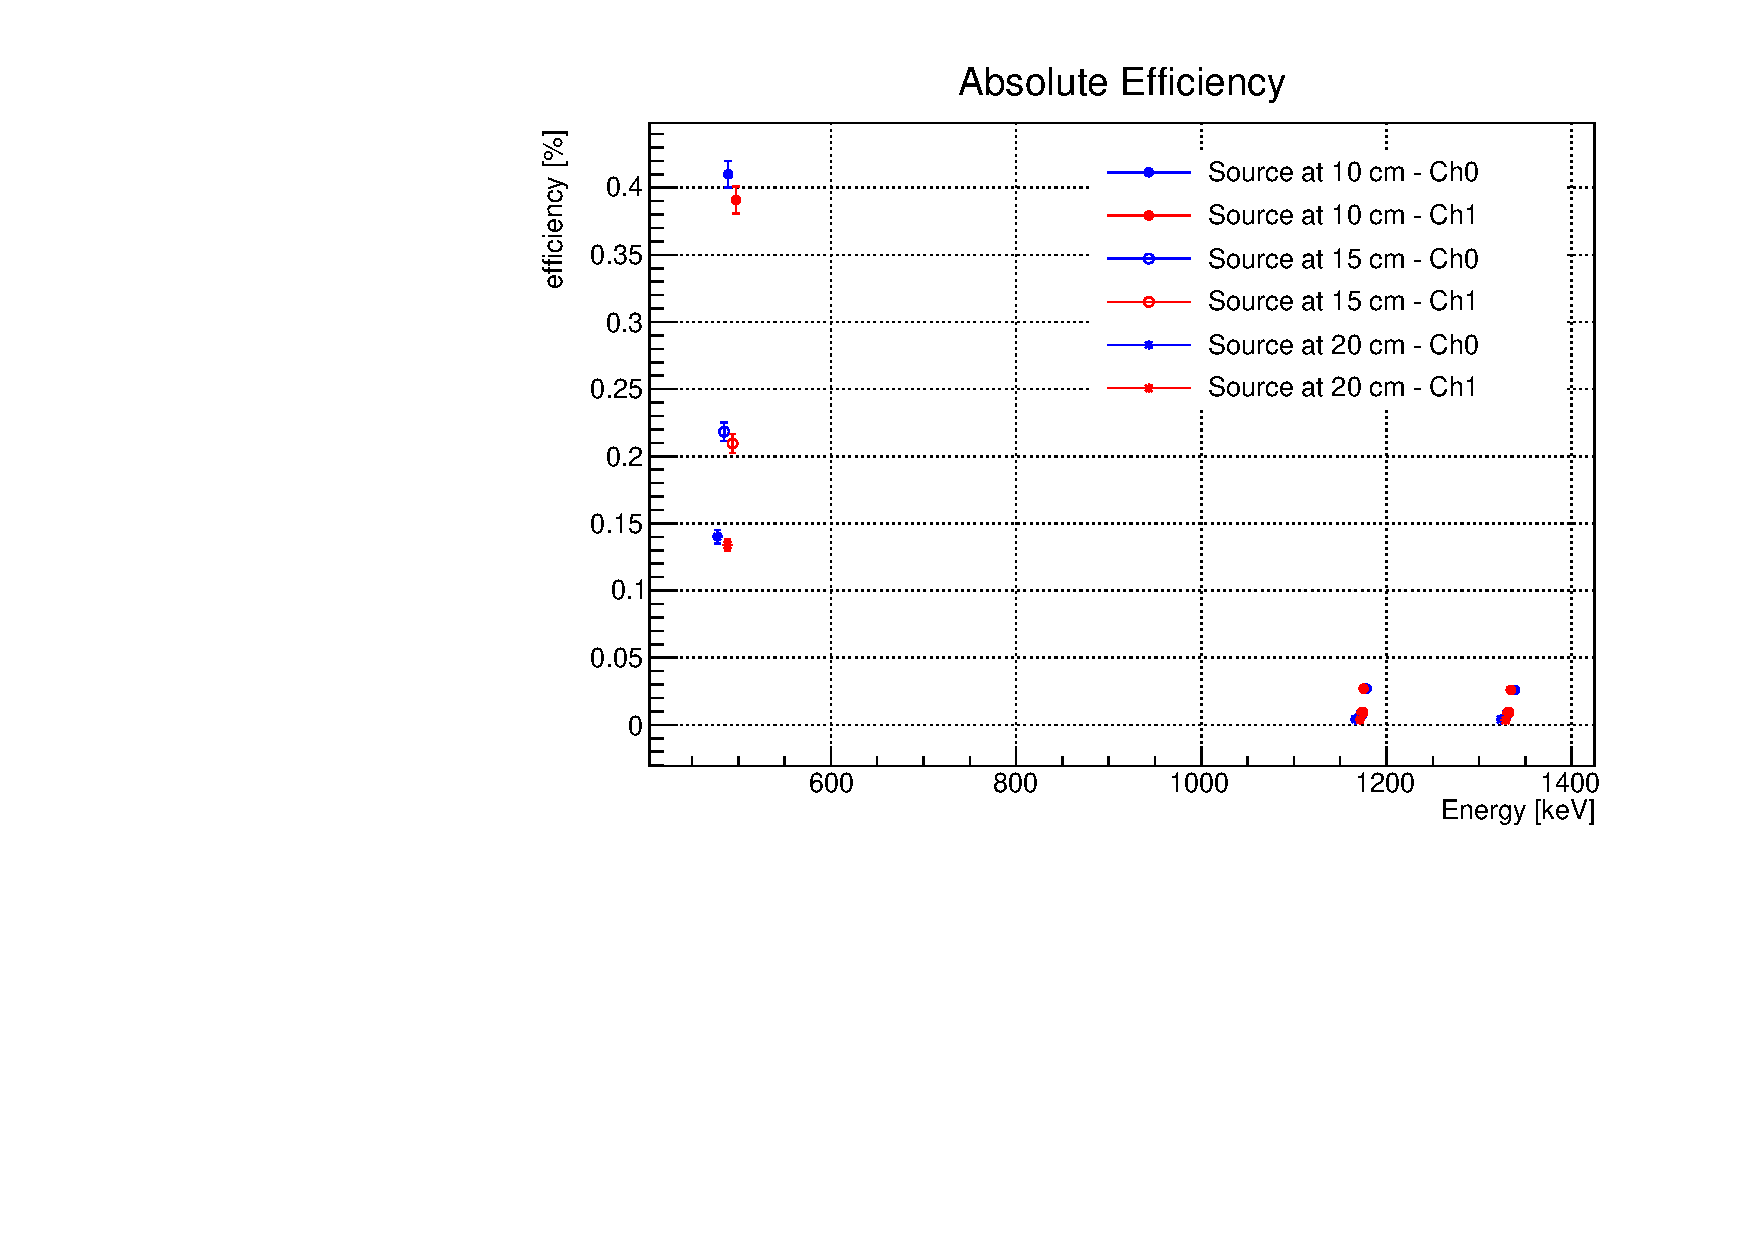
\includegraphics[scale=0.5]{Images/analysis/efficiency/Eff_coinc.pdf}
    \caption{Efficiency of the detectors, imposing coincidences and considering summing up as in \ref{eq:eta}, with detector 0 in blue and detector 1 in red, for all the distances.}
    \label{fig:eff_coinc}
\end{figure}

\begin{figure}[H]
	\begin{minipage}[c]{0.35\linewidth}
    \centering
	\subfloat[][Sources at 10 cm.]{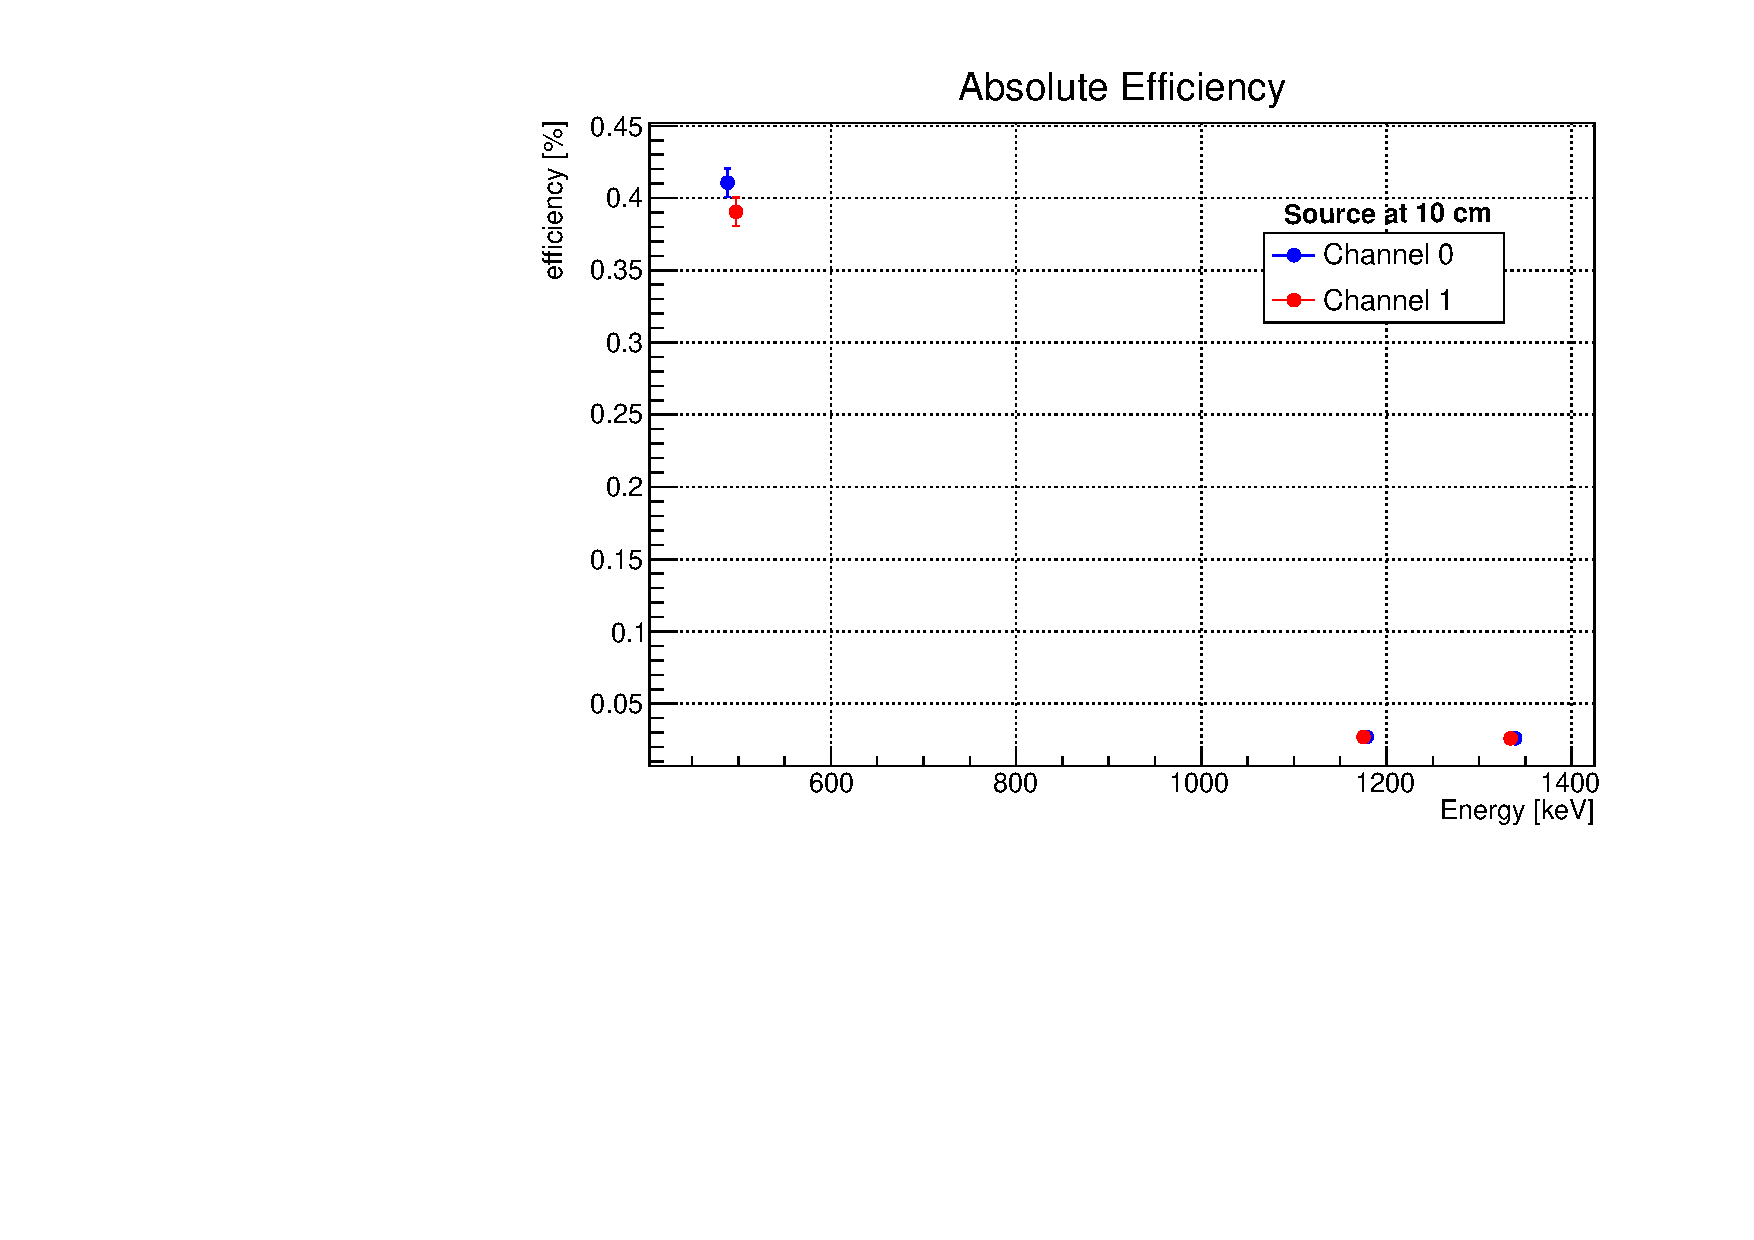
\includegraphics[width=0.95\textwidth]{Images/analysis/efficiency/eff_coinc_10.pdf} \label{fig:coinc_10} }
	\end{minipage}
	\begin{minipage}[]{0.35\linewidth}
	\centering
	\subfloat[][Sources at 15 cm.]{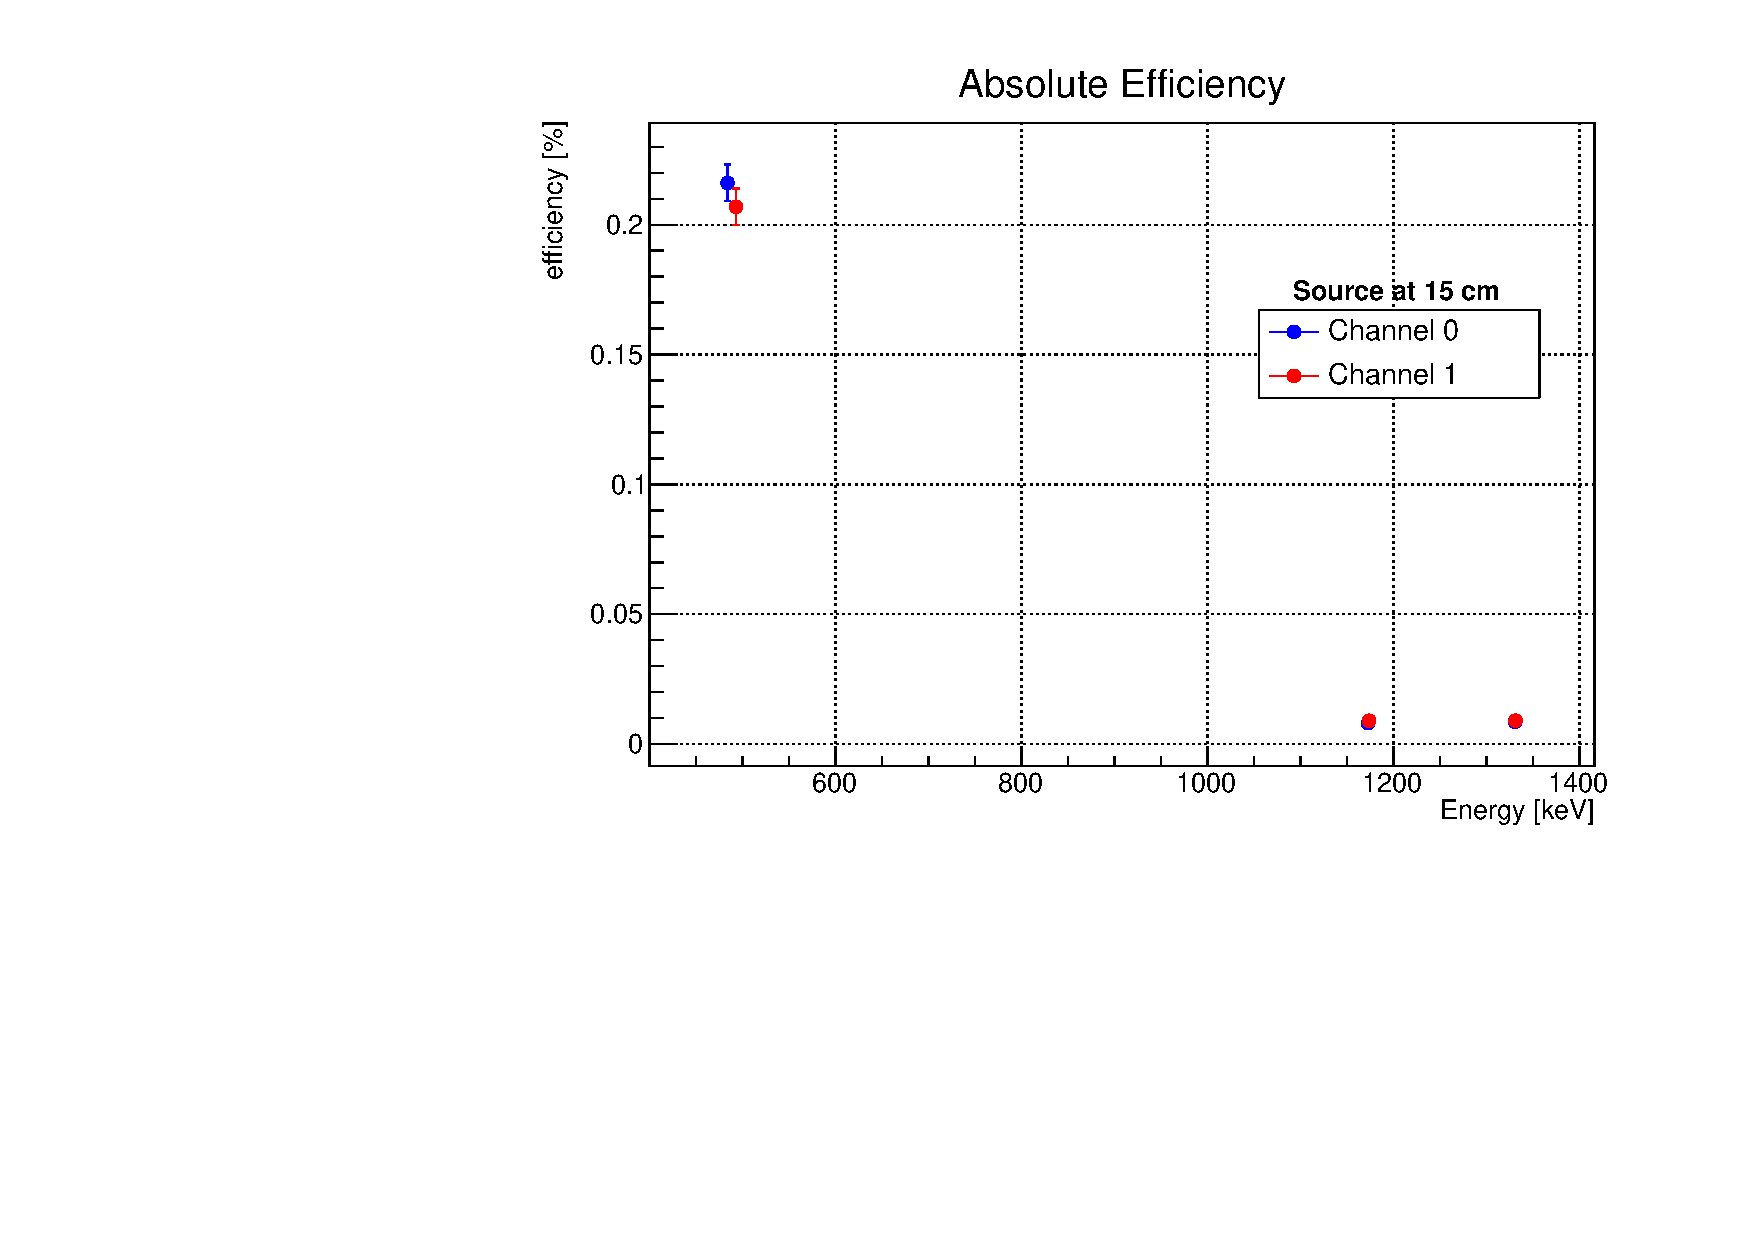
\includegraphics[width=0.95\textwidth]{Images/analysis/efficiency/eff_coinc_15.pdf}  \label{fig:coinc_15} }
	\end{minipage}
    \begin{minipage}[c]{0.35\linewidth}
    \centering
	\subfloat[][Source at 20 cm]{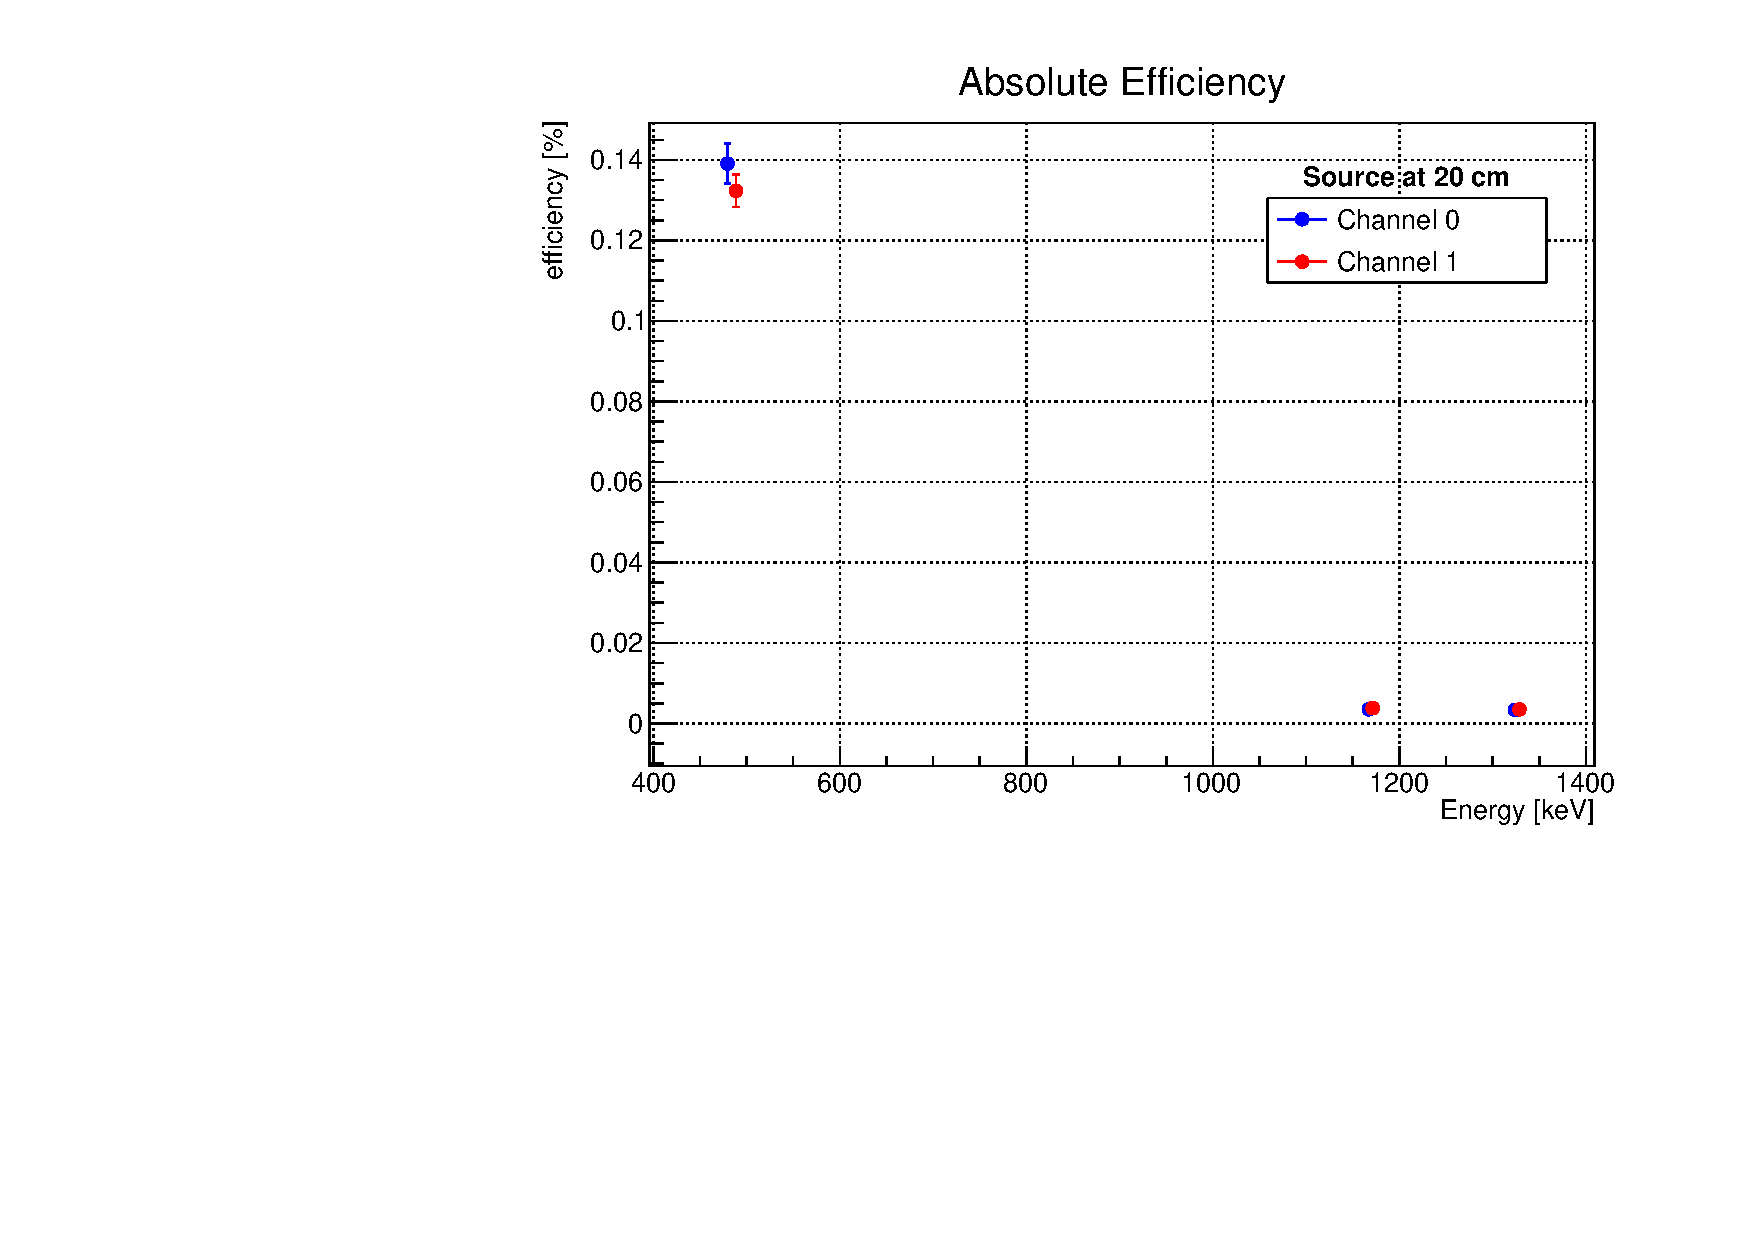
\includegraphics[width=0.95\textwidth]{Images/analysis/efficiency/eff_coinc_20.pdf}} \label{fig:coinc_20} 
	\end{minipage}
	\caption{Efficiency of the detectors, imposing coincidences and considering summing up as in \ref{eq:eta}, with detector 0 in blue and detector 1 in red, at each different distances for each plot.}
    \label{fig:eff_coinc3}
	\end{figure}


\begin{table}[h]
    \begin{subtable}
        \centering
        \begin{tabular}{|c|c|c|c|}
        \hline
        & E [keV]  & eff [\%] &$\sigma_{eff}$ [\%]  \\
        \hline
        $^{22}$Na at 10 cm & 511 &0.41&0.01\\
        \hline
        \multirow{2}{*}{$^{60}$Co at 10 cm}&1173 &0.027 & 0.001 \\ 
        &1332 &0.026 & 0.001 \\
        \hline
        $^{22}$Na at 15 cm & 511 &0.216&0.007\\
        \hline
        \multirow{2}{*}{$^{60}$Co at 15 cm}&1173 &0.008 & 0.001 \\ 
        &1332 &0.0086 & 0.0005 \\
        \hline
        $^{22}$Na at 20 cm & 511 &0.139&0.005\\
        \hline
        \multirow{2}{*}{$^{60}$Co at 20 cm}&1173 &20.0035 & 0.0003 \\
        &1332 &20.0034 & 0.0003 \\
        \hline
        \end{tabular}
    \end{subtable}
    \qquad
    \qquad
    \qquad
    \begin{subtable}
        \centering
        \begin{tabular}{|c|c|c|c|}
        \hline
        & E [keV]  & eff [\%] &$\sigma_{eff}$ [\%]  \\
        \hline
        $^{22}$Na at 10 cm & 511 &0.39&0.01\\
        \hline
        \multirow{2}{*}{$^{60}$Co at 10 cm}&1173 &0.027 & 0.001 \\ 
        &1332 &0.026 & 0.001 \\
        \hline
        $^{22}$Na at 15 cm & 511 &0.207&0.007\\
        \hline
        \multirow{2}{*}{$^{60}$Co at 15 cm}&1173 &0.009 & 0.001 \\ 
        &1332 &0.009 & 0.001 \\
        \hline
        $^{22}$Na at 20 cm & 511 &0.132&0.004\\
        \hline
        \multirow{2}{*}{$^{60}$Co at 20 cm}&1173 &0.0038 & 0.0003 \\
        &1332 &0.0035 & 0.0003 \\
        \hline
        \end{tabular}
     \end{subtable}
     \caption{Values of efficiency for the $^{60}$Co and $^{22}$Na source at different distances, imposing the coincidence between the detectors, for detector 0 and 1, respectively.}
     \label{table:eff_coin}
\end{table}


\subsection{With Coincidences and Condition on Energy}

To have a more refined efficiency we can impose a condition on the energy. In particular, we want to see the energy spectrum of a detector (b) when the other (a) sees a particular gamma. In this way the number of emitted events used to calculate the efficiency is not the number of events produced by the source, but is the number of events in an energy range detected by detector a. To do this calculation we plot the energy spectrum of detector b (fig. \ref{fig:coinc_spectra_all}-\ref{fig:coinc_spectra_all_log}), when we have temporal coincidences and when the other detector (a) registers events within $2\sigma$ from the value of the peak of interest. We then calculate the area of the peak of the spectrum for detector b with the condition required, as the number of detected events and we divide it by the number of events in the energy range of the spectrum of detector a, obtaining the efficiencies shown in tab. \ref{tab:eff_coin_en} and in fig. \ref{fig:eff_all}. \\

We can see that the values of efficiencies for $^{22}$Na, despite the source being moved further away, remain roughly the same. This is due to the fact that we are taking the ratio of events between the two detectors, so even though the solid angle subtended by the single detectors gets smaller, the two geometric factors cancel each other out and the efficiency remains constant.
This is not true for $^{60}$Co, as the photons are not necessarily emitted in opposite directions so the decreasing solid angle plays a role.  

\begin{figure}[H]
	\begin{minipage}[c]{0.5\linewidth}
	\subfloat[][$^{60}$Co source at 10 cm.]{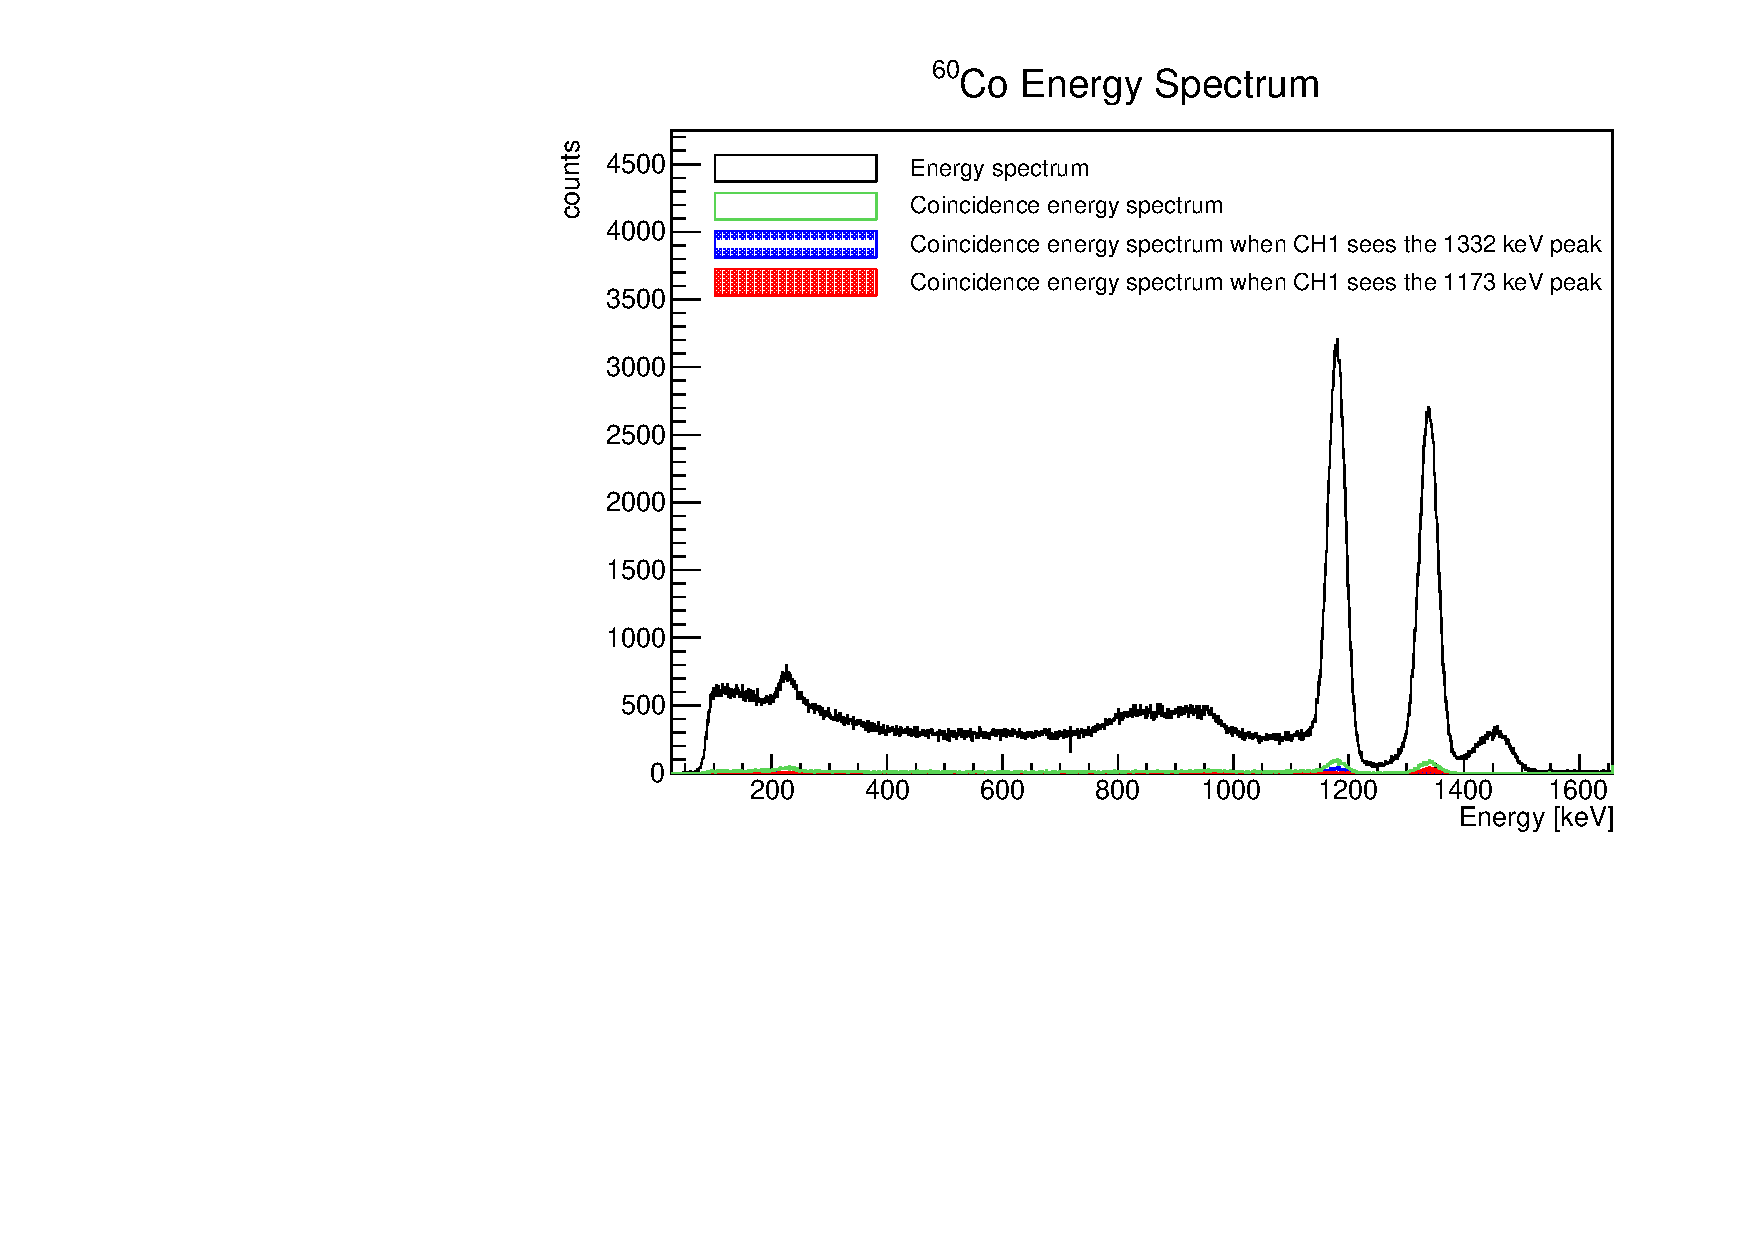
\includegraphics[width=0.9\textwidth]{Images/analysis/efficiency/Co_coinc_all.pdf} \label{fig:Co_all} }
	\end{minipage}
	\begin{minipage}[]{0.5\linewidth}
	\centering
	\subfloat[][$^{22}$Na source at 10 cm.]{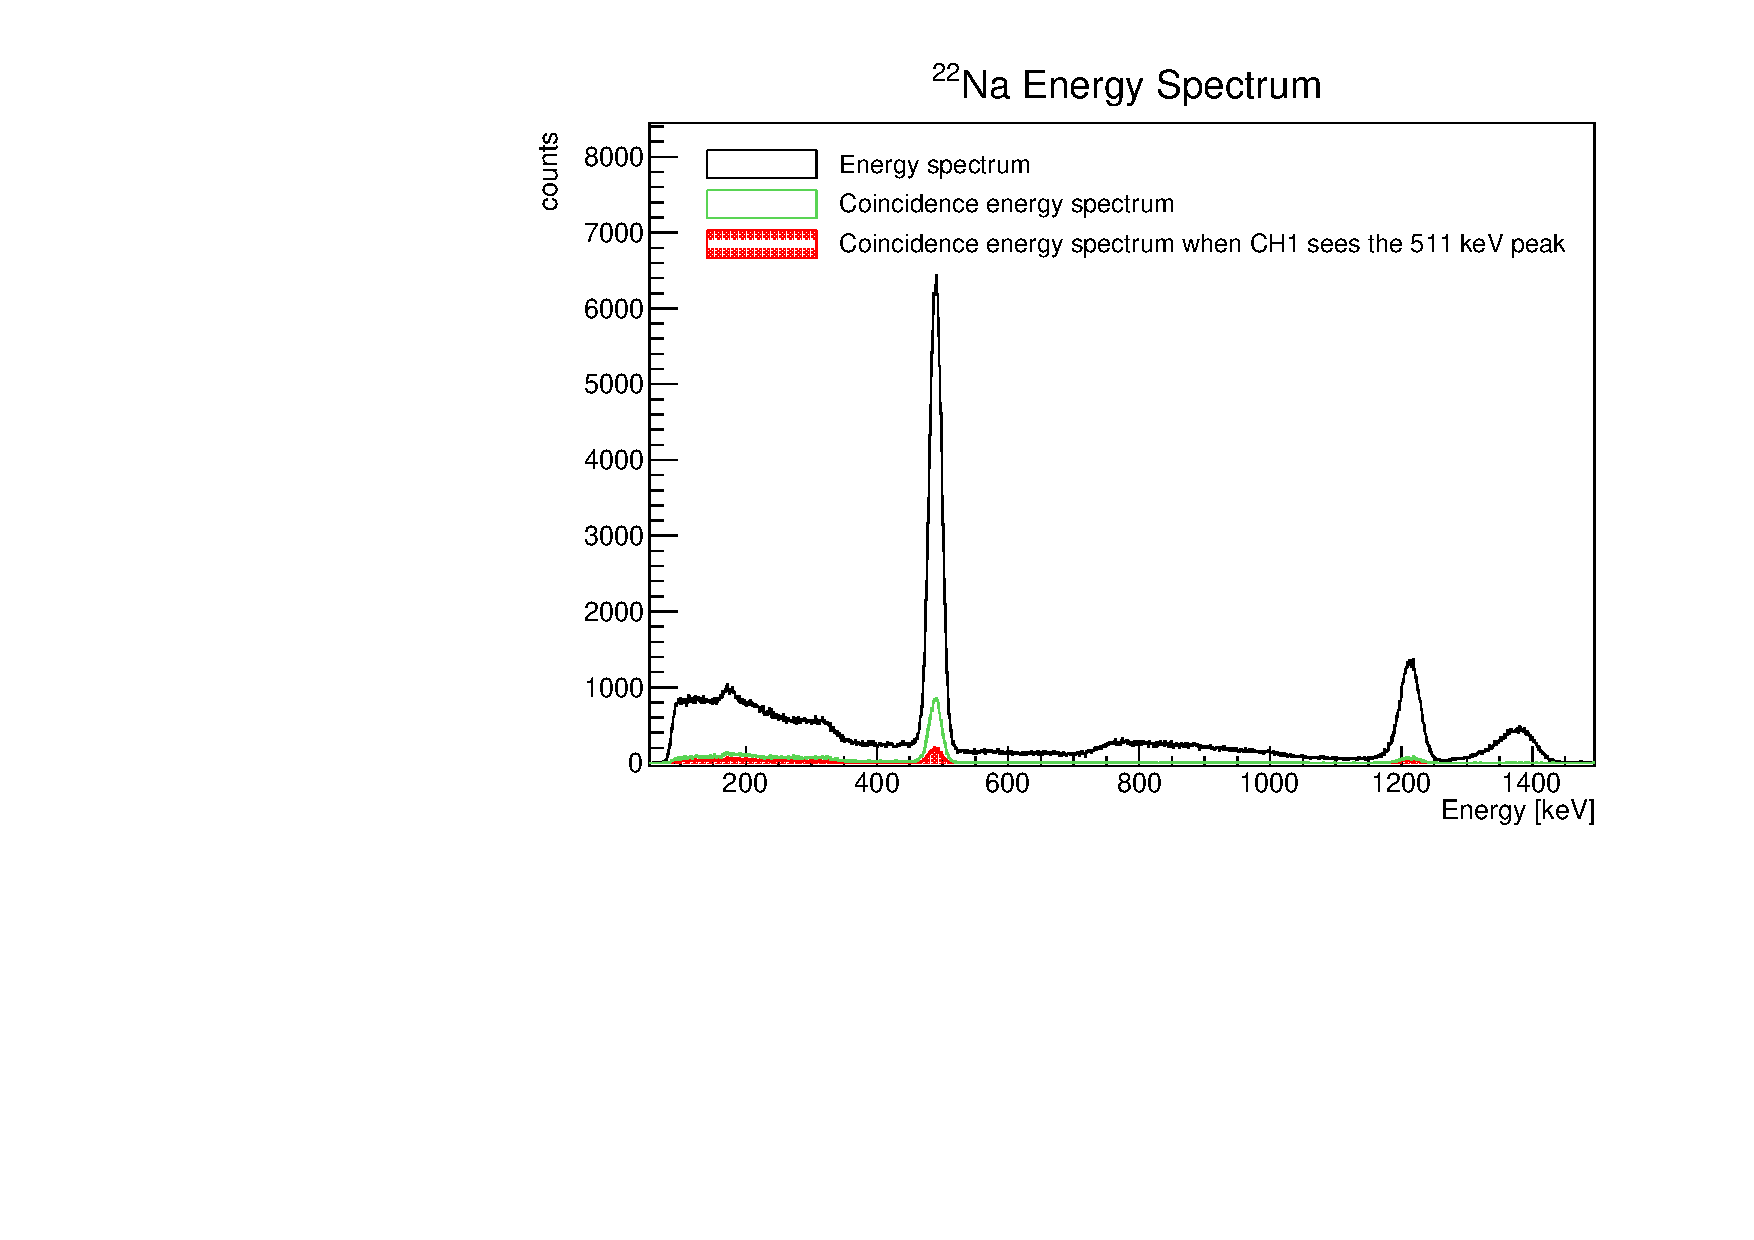
\includegraphics[width=0.9\textwidth]{Images/analysis/efficiency/Na_coinc_all.pdf}  \label{fig:Na_all} }
	\end{minipage}
	\caption{Comparison between the initial energy spectra of $^{60}$Co and $^{22}$Na, in black, the energy spectra obtained imposing coincidence between the two detectors in green, and the spectra obtained imposing the energy condition on the other detector, in red (and blue). Both spectra regard detector 0.}
    \label{fig:coinc_spectra_all}
	\end{figure}

\begin{figure}[H]
	\begin{minipage}[c]{0.5\linewidth}
	\subfloat[][$^{60}$Co source at 10 cm.]{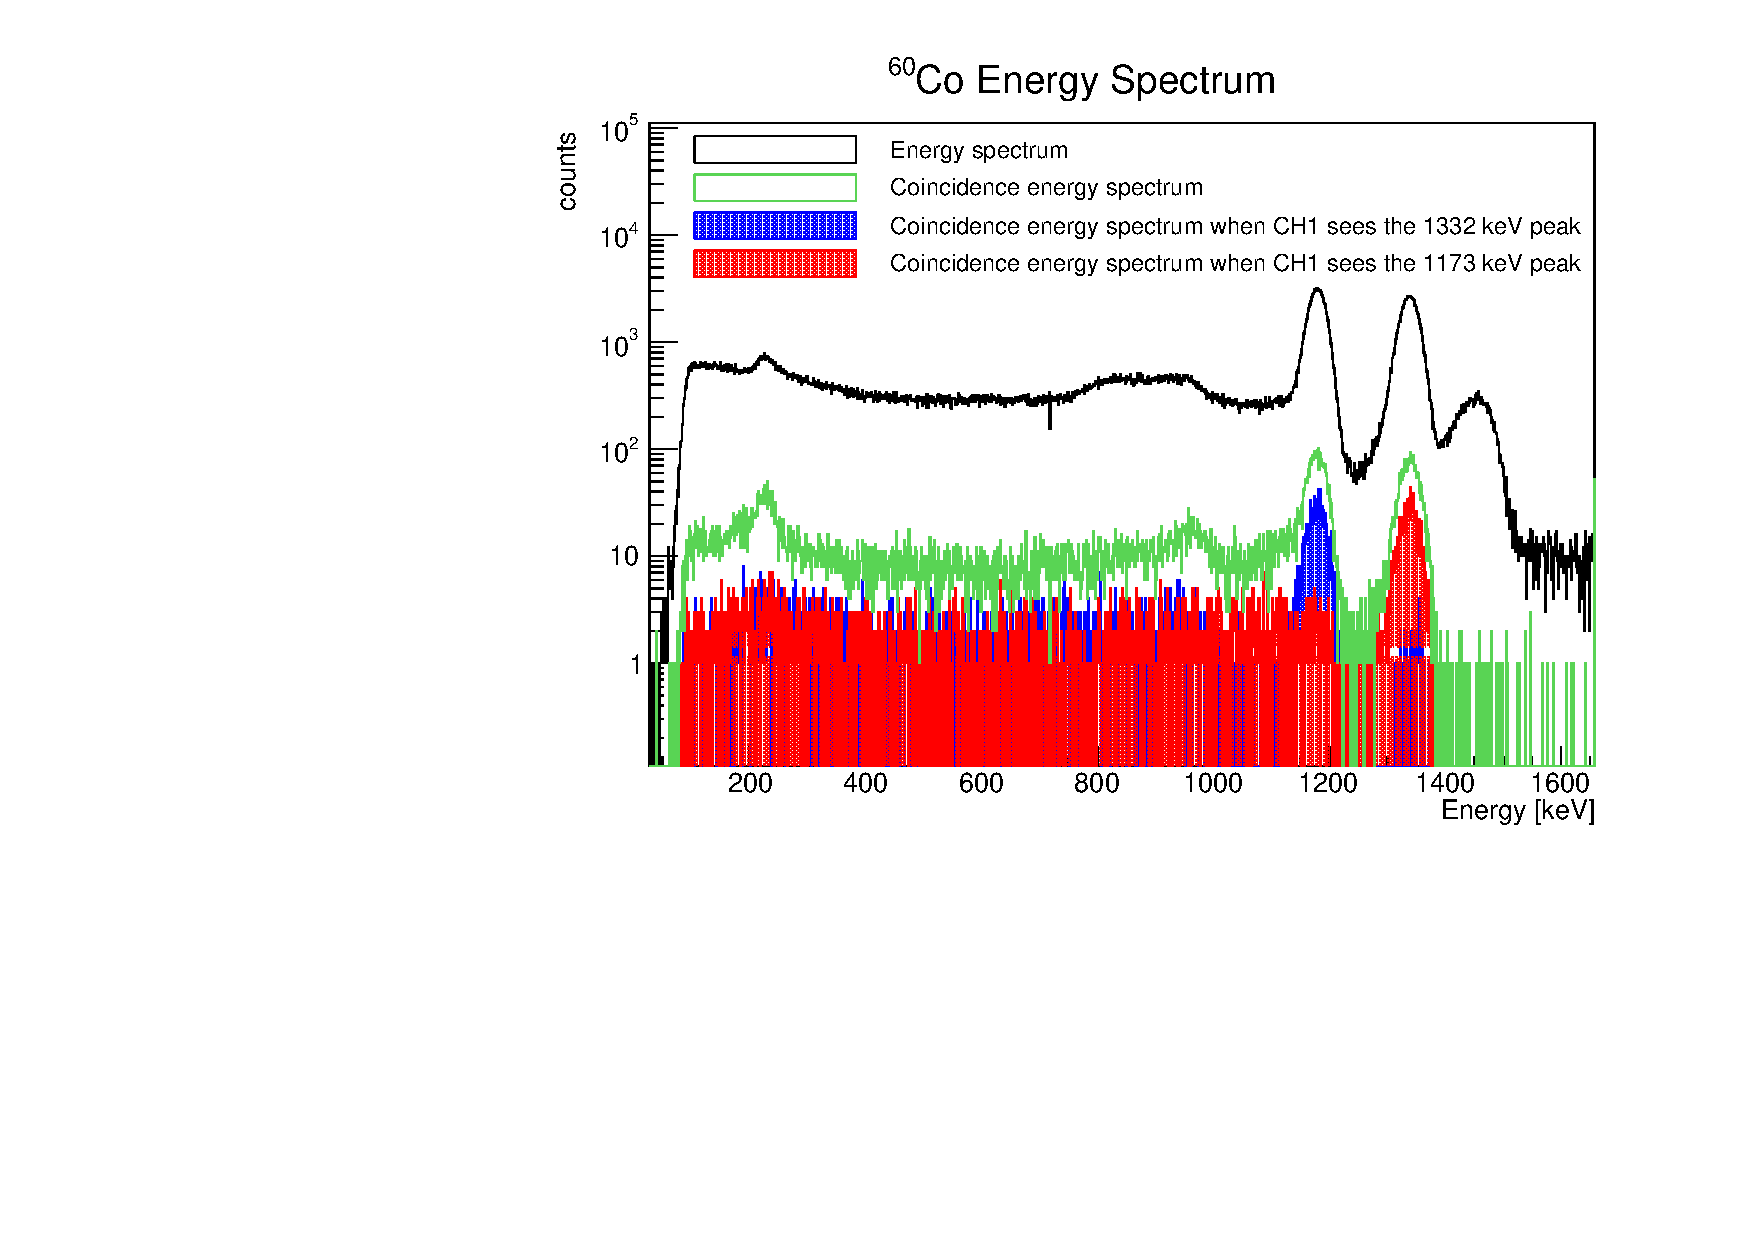
\includegraphics[width=0.9\textwidth]{Images/analysis/efficiency/Co_coinc_all_log.pdf} \label{fig:Co_all_log} }
	\end{minipage}
	\begin{minipage}[]{0.5\linewidth}
	\centering
	\subfloat[][$^{22}$Na source at 10 cm.]{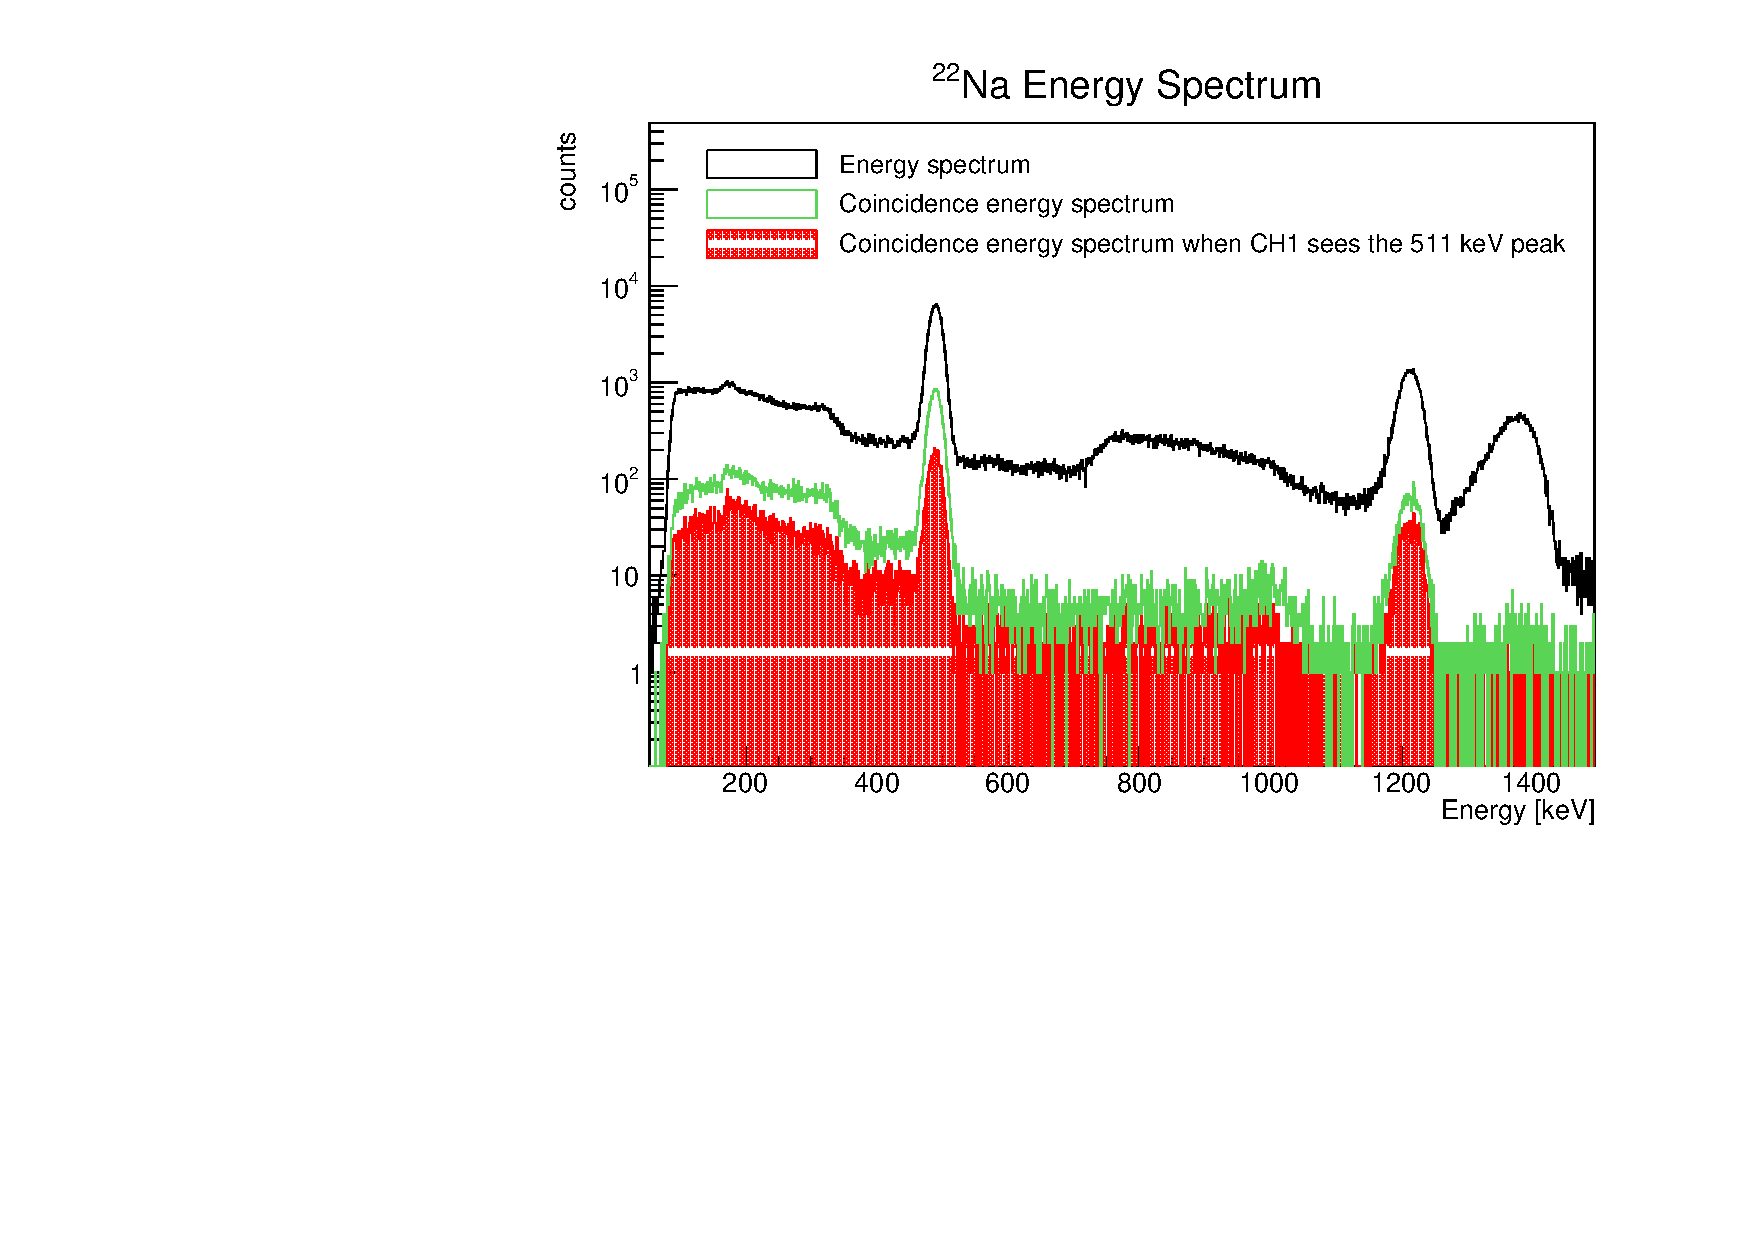
\includegraphics[width=0.9\textwidth]{Images/analysis/efficiency/Na_coinc_all_log.pdf}  \label{fig:Na_all_} }
	\end{minipage}
	\caption{Comparison between the initial energy spectra of $^{60}$Co and $^{22}$Na, in black, the energy spectra obtained imposing coincidence between the two detectors in green, and the spectra obtained imposing the energy condition on the other detector, in red (and blue). Both spectra regard detector 0.}
    \label{fig:coinc_spectra_all_log}
	\end{figure}

\begin{table}[h]
    \begin{subtable}
        \centering
        \begin{tabular}{|c|c|c|c|}
        \hline
        & E [keV]  & eff [\%] &$\sigma_{eff}$ [\%]  \\
        \hline
        $^{22}$Na at 10 cm & 511 & 2.56 & 0.08 \\
        \hline
        \multirow{2}{*}{$^{60}$Co at 10 cm}&1173 &0.92 & 0.03 \\ 
        &1332 &0.76 & 0.03 \\
        \hline
        $^{22}$Na at 15 cm & 511 & 2.47 & 0.08 \\
        \hline
        \multirow{2}{*}{$^{60}$Co at 15 cm}&1173 &0.50 & 0.02 \\ 
        &1332 &0.42 & 0.02 \\
        \hline
        $^{22}$Na at 20 cm & 511 & 2.48 & 0.08 \\
        \hline
        \multirow{2}{*}{$^{60}$Co at 20 cm}&1173 &0.24 & 0.02 \\
        &1332 &0.24& 0.02 \\
        \hline
        \end{tabular}
    \end{subtable}
    \qquad
    \qquad
    \qquad
    \begin{subtable}
        \centering
        \begin{tabular}{|c|c|c|c|}
        \hline
        & E [keV]  & eff [\%] &$\sigma_{eff}$ [\%]  \\
        \hline
        $^{22}$Na at 10 cm & 511 & 2.52 & 0.08 \\
        \hline
        \multirow{2}{*}{$^{60}$Co at 10 cm}&1173 &0.97 &0.03 \\ 
        &1332 &0.83 & 0.03 \\
        \hline
        $^{22}$Na at 15 cm & 511 & 2.47 & 0.08 \\
        \hline
        \multirow{2}{*}{$^{60}$Co at 15 cm}&1173 &0.53 & 0.02 \\ 
        &1332 &0.47 & 0.02 \\
        \hline
        $^{22}$Na at 20 cm & 511 & 2.51 & 0.08 \\
        \hline
        \multirow{2}{*}{$^{60}$Co at 20 cm}&1173 &0.28 & 0.02 \\
        &1332 &0.21 & 0.01 \\
        \hline
        \end{tabular}
     \end{subtable}
     \caption{Values of efficiency for the $^{60}$Co source at different distances, imposing the coincidence between the detectors and the condition that in the other we see the other peak, for detector 0 and 1 respectively}
     \label{tab:eff_coin_en}
\end{table}

\begin{figure}[H]
    \centering
    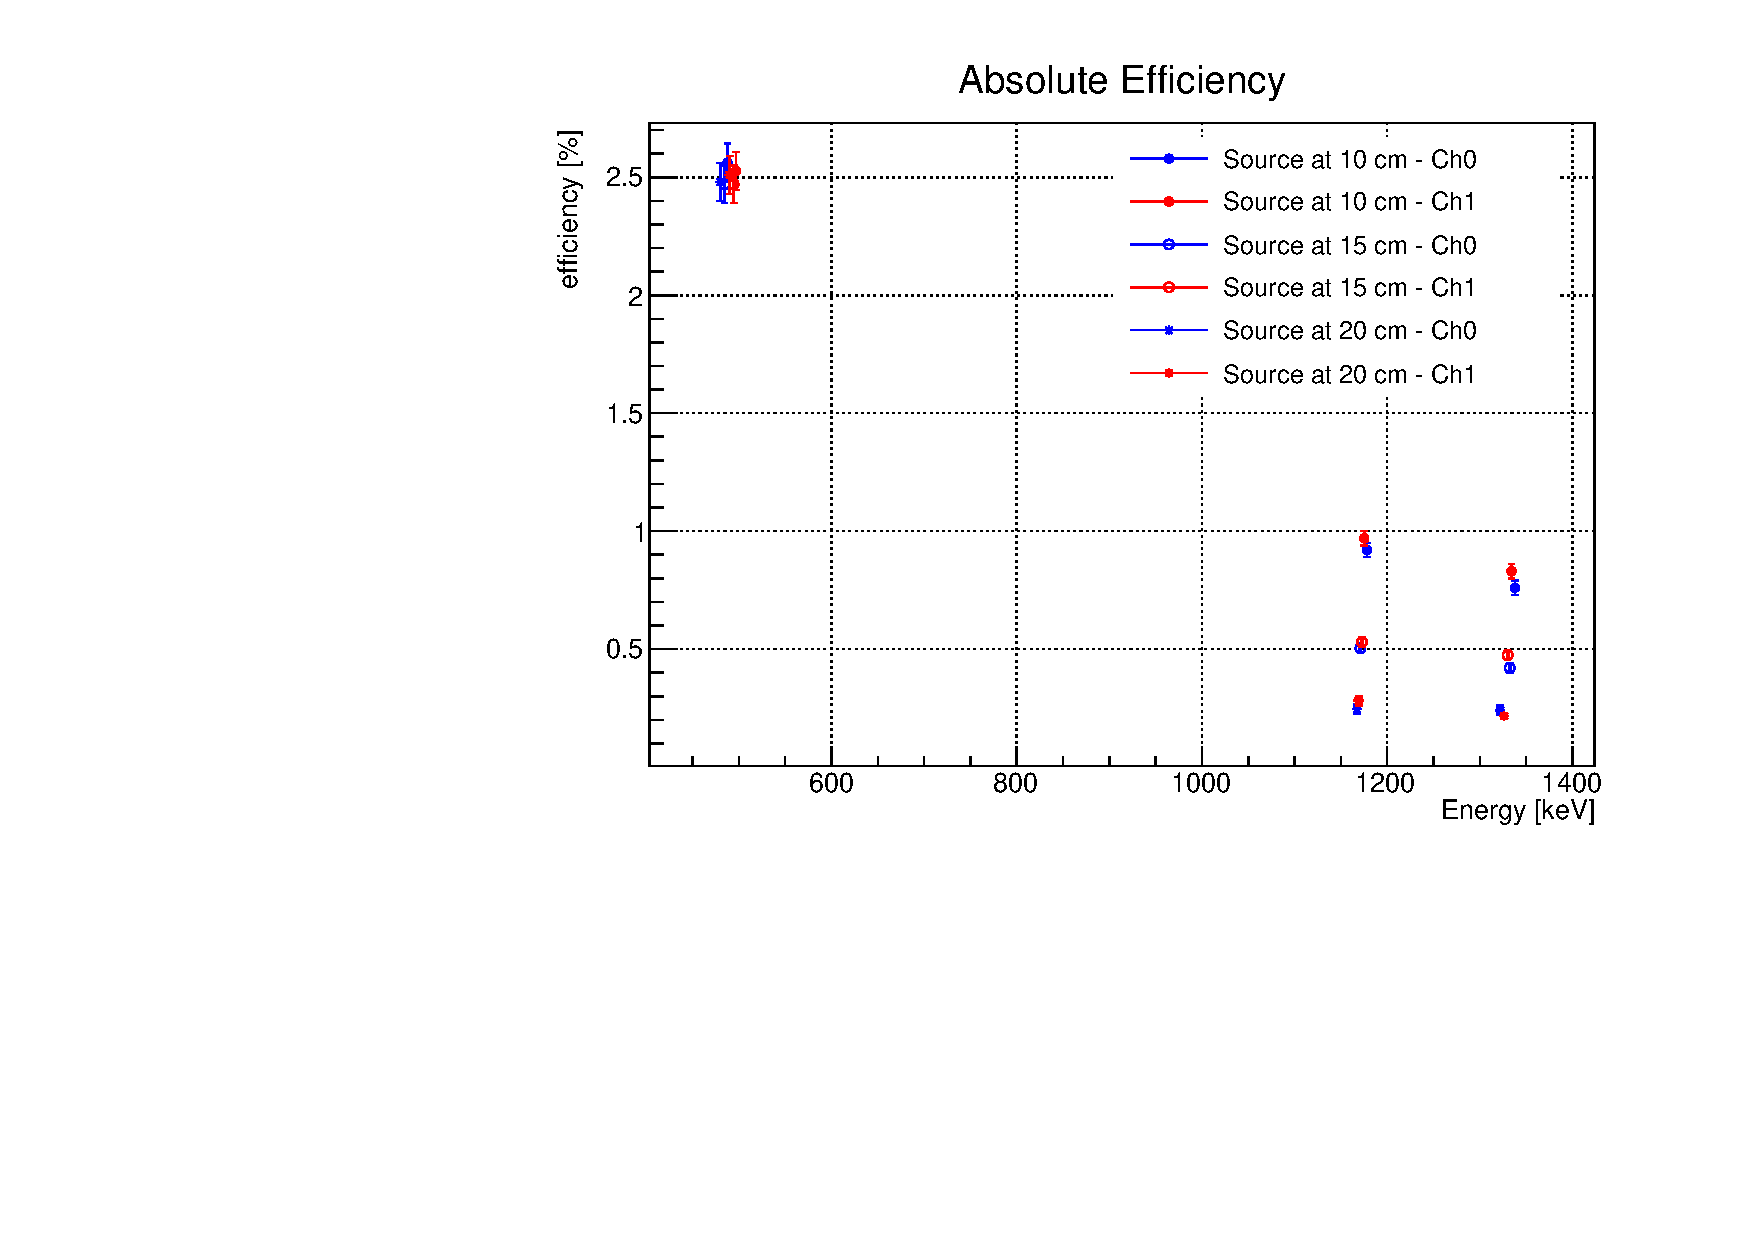
\includegraphics[scale=0.5]{Images/analysis/efficiency/Eff_all.pdf}
    \caption{Efficiency of the detectors, imposing coincidences, energy condition and considering summing up as in \ref{eq:eta}, with detector 0 in blue and detector 1 in red, for all the distances.}
    \label{fig:eff_all}
\end{figure}

\begin{figure}[H]
	\begin{minipage}[c]{0.35\linewidth}
    \centering
	\subfloat[][Sources at 10 cm.]{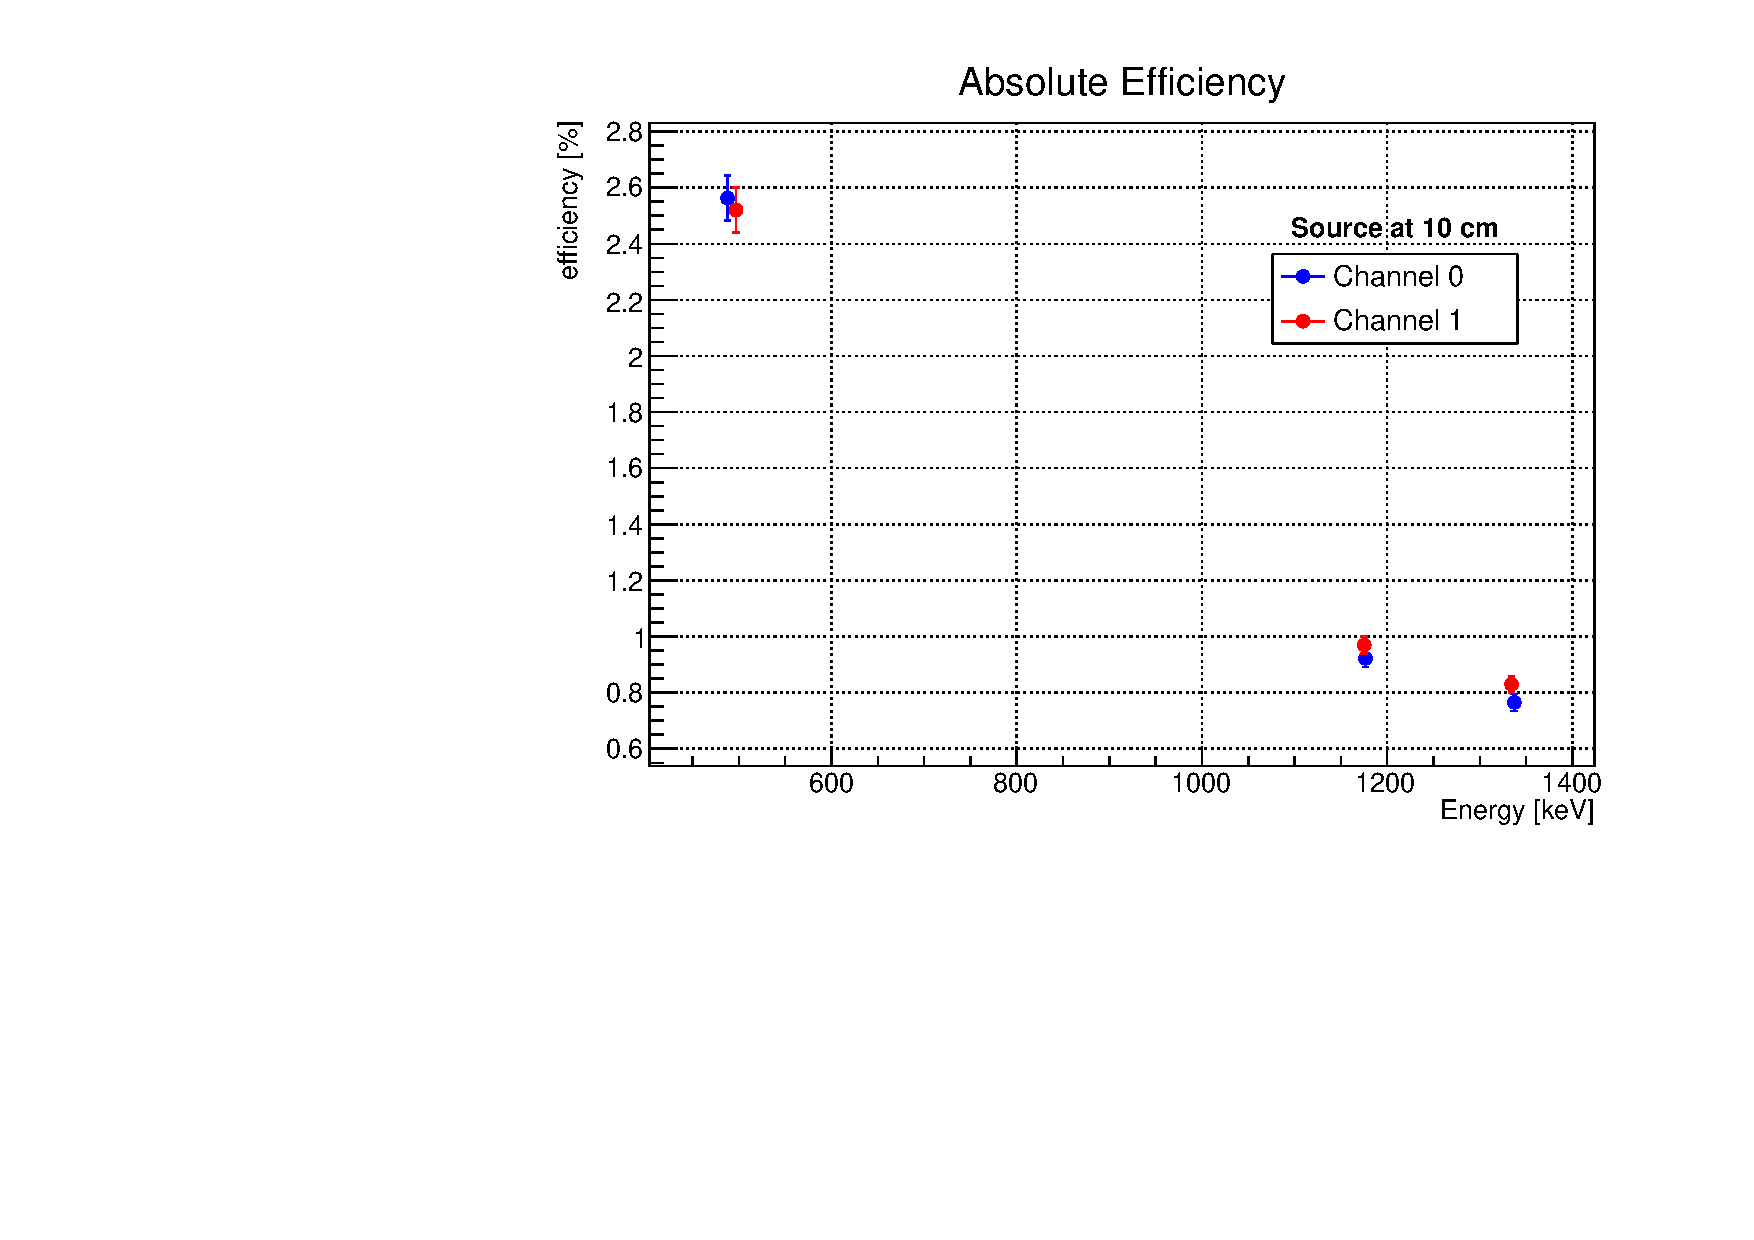
\includegraphics[width=0.95\textwidth]{Images/analysis/efficiency/eff_all_10.pdf}\label{fig:all_10} }
	\end{minipage}
	\begin{minipage}[]{0.35\linewidth}
	\centering
	\subfloat[][Sources at 15 cm.]{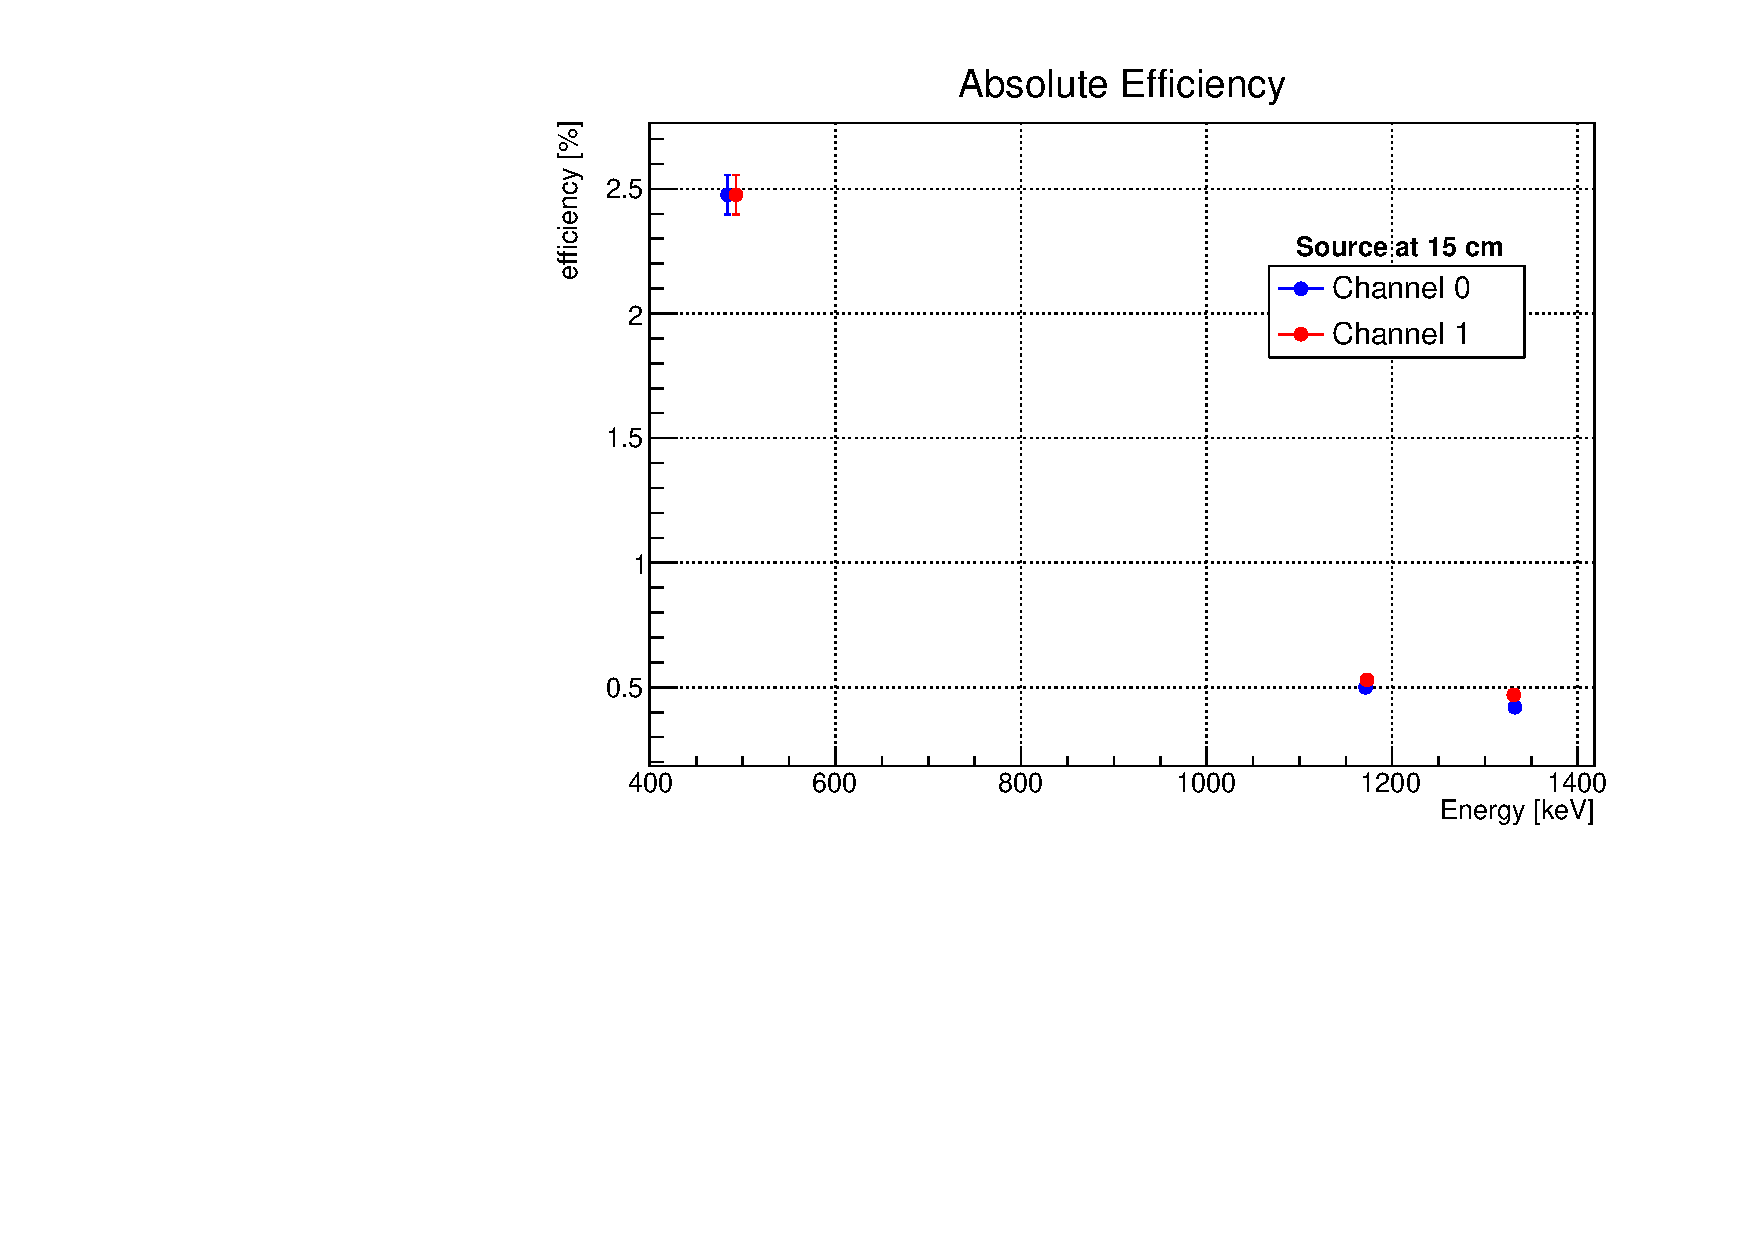
\includegraphics[width=0.95\textwidth]{Images/analysis/efficiency/eff_all_15.pdf}  \label{fig:all_15} }
	\end{minipage}
    \begin{minipage}[c]{0.35\linewidth}
    \centering
	\subfloat[][Source at 20 cm]{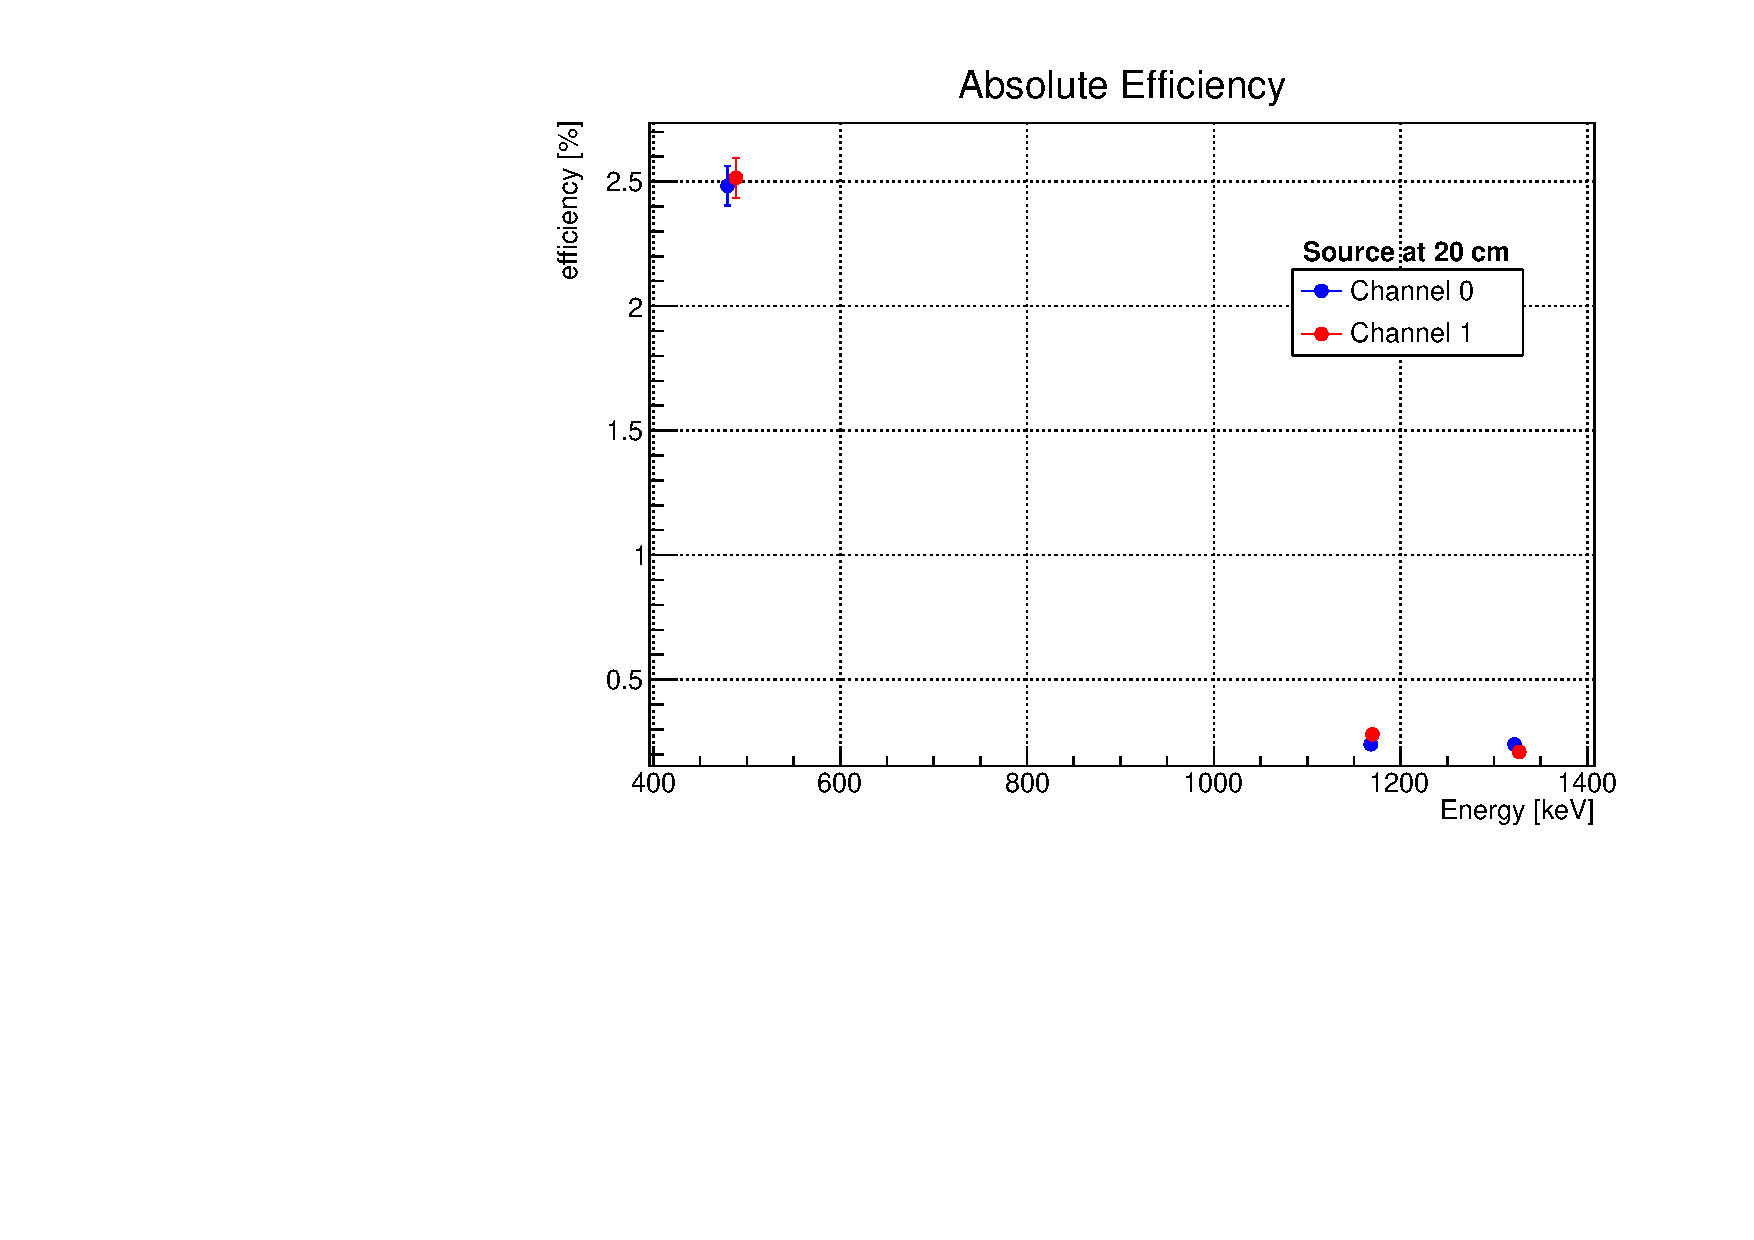
\includegraphics[width=0.95\textwidth]{Images/analysis/efficiency/eff_all_20.pdf}\label{fig:all_20}} 
	\end{minipage}
	\caption{Efficiency of the detectors, imposing coincidences, energy condition and considering summing up as in \ref{eq:eta}, with detector 0 in blue and detector 1 in red, at each different distances for each plot.}
    \label{fig:eff_all3}
	\end{figure}

     









%	% To insert two subfigure
%	\begin{figure}[H]
%	\begin{minipage}[c]{0.49\linewidth}
%	\subfloat[][Description of the subfigure]{\includegraphics[width=0.8\textwidth]{image/prova.jpg} \label{fig:2_prova_a} }
%	\end{minipage}
%	\begin{minipage}[]{0.49\linewidth}
%	\centering
%	\subfloat[][Description of the subfigure]{\includegraphics[width=0.8\textwidth]{image/prova.jpg}  \label{fig:2_prova_b} }
%	\end{minipage}
%	\caption{\label{fig:2_prova} In \ref{fig:2_prova_a} ..., while \ref{fig:2_prova_b} shows... }
%	\end{figure}
%	
%	% To insert four subfigure
%	\begin{figure}[H]
%	\begin{minipage}[c]{0.49\linewidth}
%	\subfloat[][Description of the subfigure]{\includegraphics[width=0.8\textwidth]{image/prova.jpg} \label{fig:3_prova_a} }
%	\end{minipage}
%	\begin{minipage}[]{0.49\linewidth}
%	\centering
%	\subfloat[][Description of the subfigure]{\includegraphics[width=0.8\textwidth]{image/prova.jpg} \label{fig:3_prova_b} }
%	\end{minipage} \\
%	\vfill
%	\begin{minipage}[c]{0.49\linewidth}
%	\subfloat[][Description of the subfigure]{\includegraphics[width=0.8\textwidth]{image/prova.jpg} \label{fig:3_prova_c} }
%	\end{minipage}
%	\begin{minipage}[]{0.49\linewidth}
%	\centering
%	\subfloat[][Description of the subfigure]{\includegraphics[width=0.8\textwidth]{image/prova.jpg} \label{fig:3_prova_d} }
%	\end{minipage}
%	\caption{\label{fig:3_prova} In \ref{fig:3_prova_a} ..., \ref{fig:3_prova_b} shows..., \ref{fig:3_prova_c} and \ref{fig:3_prova_d}...  }
%	\end{figure}
	
	
	% Example to insert a well-formatted table
%   	\begin{table}[H]
%	\centering
%   	 \sisetup{separate-uncertainty}
%   	 \begin{tabular*}{\linewidth}{@{\extracolsep{\fill}}
%   	 l 
%   	 l 
%   	 S[table-format=3(1)]  %intercept
%   	 S[table-format=1.2(2)] %slope
%   	 S[table-format=1.3]
%   	 l 
%   	 l 
%  	 c 
%  	 c  
%  	}
%        \toprule
%    & \textbf{Linear fit} & \textbf{ Intercept [mV] }  & \textbf{ Slope [mV/K] } & $\pmb{r}$ & \textbf{$\pmb{\chi^{(2)}}$/ndf} & \textbf{p-value} & \textbf{$\pmb{T_c}$ [K]} & \textbf{$\pmb{V(T_c)}$ [mV]}\\
%        \colrule
%    \multirow{2}{*}{{\color{cool}\textbf{Cooling}}} & $\pmb{a_l + b_l \, x }$ &  453\pm3   &   -1.11\pm0.04 & -0.845 & 198.3/61 & $2 \cdot 10^{-16}$ & \multirow{2}{*}{ \tablenum{80\pm1}} & \multirow{2}{*}{ \tablenum{ 363\pm5} } \\
%     & $\pmb{a_r + b_r \, x }$ &  99\pm22   &  3.3\pm0.3  & 0.896 & 90.36/17 & $5 \cdot 10^{-12}$\\
%         \colrule
%    \multirow{2}{*}{{\color{hot}\textbf{Heating}}} & $\pmb{a_l + b_l \, x }$ &  521 \pm 5   &   -1.19 \pm 0.05 & -0.940 & 54.72/57 & 0.561 & \multirow{2}{*}{ \tablenum{ 109 \pm 3}} & \multirow{2}{*}{ \tablenum{ 392\pm8} } \\
%     & $\pmb{a_r + b_r \, x }$ &  173\pm10   &  2.01\pm0.09  & 0.915 & 47.81/33& 0.046\\ 
%    \botrule
%    \end{tabular*}
%    \caption{Description ...}
%    \label{tab:1_tab}
%    \end{table}
	

\section{Conclusions}
\label{sec:conclusions}

 In this work two LaBr scintillating detectors were completely characterised using $^{22}$Na, $^{137}$Cs and $^{60}$Co radioactive sources as references. \\
 First we calibrated them by computing the relation between actual energy and readout channel. Later we studied their energy resolution as a function of the energy and their timing performances. Finally, the efficiency at different energies was studied using different techniques.

% To add bibliography (file references.bib)
\bibliographystyle{plain}
\bibliography{references}{}

\end{document}
